%%%%%%%%%%%%%%%%%%%%%%%%%%%%%%%%%%%%%%%%%%%%%%%%%%%%%%%%%%%%%%%%%%%%%%%%%%%%%%%%%%%%%%%%%%%%%%%%%%%%%%%%%%%%%%%%%%%%%%%%%%%%%%%%%%%%%%%%%%%%%%%%%%%%%%%%%%%
% This is just an example/guide for you to refer to when submitting manuscripts to Frontiers, it is not mandatory to use Frontiers .cls files nor frontiers.tex  %
% This will only generate the Manuscript, the final article will be typeset by Frontiers after acceptance.   
%                                              %
%                                                                                                                                                         %
% When submitting your files, remember to upload this *tex file, the pdf generated with it, the *bib file (if bibliography is not within the *tex) and all the figures.
%%%%%%%%%%%%%%%%%%%%%%%%%%%%%%%%%%%%%%%%%%%%%%%%%%%%%%%%%%%%%%%%%%%%%%%%%%%%%%%%%%%%%%%%%%%%%%%%%%%%%%%%%%%%%%%%%%%%%%%%%%%%%%%%%%%%%%%%%%%%%%%%%%%%%%%%%%%

%%% Version 3.4 Generated 2022/06/14 %%%
%%% You will need to have the following packages installed: datetime, fmtcount, etoolbox, fcprefix, which are normally inlcuded in WinEdt. %%%
%%% In http://www.ctan.org/ you can find the packages and how to install them, if necessary. %%%
%%%  NB logo1.jpg is required in the path in order to correctly compile front page header %%%

\documentclass[utf8]{FrontiersinHarvard} % for articles in journals using the Harvard Referencing Style (Author-Date), for Frontiers Reference Styles by Journal: https://zendesk.frontiersin.org/hc/en-us/articles/360017860337-Frontiers-Reference-Styles-by-Journal
%\documentclass[utf8]{FrontiersinVancouver} % for articles in journals using the Vancouver Reference Style (Numbered), for Frontiers Reference Styles by Journal: https://zendesk.frontiersin.org/hc/en-us/articles/360017860337-Frontiers-Reference-Styles-by-Journal
%\documentclass[utf8]{frontiersinFPHY_FAMS} % Vancouver Reference Style (Numbered) for articles in the journals "Frontiers in Physics" and "Frontiers in Applied Mathematics and Statistics" 

%\setcitestyle{square} % for articles in the journals "Frontiers in Physics" and "Frontiers in Applied Mathematics and Statistics" 
\usepackage{url,hyperref,lineno,microtype,subcaption}
\hypersetup{colorlinks=true,bookmarksnumbered,pdfborder={0 0 0.25}}
% ,citebordercolor={0.2667 0.4667 0.6667},citecolor=bluepurple,linkbordercolor={0.6667 0.2 0.4667},linkcolor=redpurple,urlbordercolor={0.1333 0.5333 0.2},urlcolor=green,breaklinks=true}
% \usepackage[vertfit=local]{breakurl}% only for arXiv
%% NOTE: Frontiers in Human Neuroscience does allow numbered sections, see for example
%% https://www.frontiersin.org/articles/10.3389/fnhum.2022.1032724/full
%% https://www.frontiersin.org/articles/10.3389/fnhum.2022.1077416/full
%% Other examples in the 2022 volume also show free section naming.
%
% In case of non-numbered sections:
% \makeatletter
% \AtBeginDocument{%
%   \@ifdefinable{\myorg@nameref}{%
%     \LetLtxMacro\myorg@nameref\nameref
%     \DeclareRobustCommand*{\nameref}[1]{%
%       \textbf{\color{green}\myorg@nameref{#1}}%
%     }%
%   }%
% }
% \makeatother

\usepackage[onehalfspacing]{setspace}
\usepackage[usenames]{xcolor}
% Tol (2012) colour-blind-, print-, screen-friendly colours, alternative scheme; Munsell terminology
\definecolor{bluepurple}{RGB}{68,119,170}
\definecolor{blue}{RGB}{102,204,238}
\definecolor{green}{RGB}{34,136,51}
\definecolor{yellow}{RGB}{204,187,68}
\definecolor{red}{RGB}{238,102,119}
\definecolor{redpurple}{RGB}{170,51,119}
\definecolor{grey}{RGB}{187,187,187}
\definecolor{lgrey}{RGB}{221,221,221}

\definecolor{notecolour}{RGB}{68,170,153}
%\newcommand*{\puzzle}{\maltese}
\newcommand*{\puzzle}{{\fontencoding{U}\fontfamily{fontawesometwo}\selectfont\symbol{225}}}
\newcommand*{\wrench}{{\fontencoding{U}\fontfamily{fontawesomethree}\selectfont\symbol{114}}}
\newcommand*{\pencil}{{\fontencoding{U}\fontfamily{fontawesometwo}\selectfont\symbol{210}}}
\newcommand{\mynotew}[1]{{\color{notecolour}\wrench\ #1}}
\newcommand{\mynotep}[1]{{\color{notecolour}\pencil\ #1}}
\newcommand{\mynotez}[1]{{\color{notecolour}\puzzle\ #1}}

\usepackage{wrapfig}



\providecommand{\href}[2]{#2}
\providecommand{\eprint}[2]{\texttt{\href{#1}{#2}}}
\newcommand*{\amp}{\&}
% \newcommand*{\citein}[2][]{\textnormal{\textcite[#1]{#2}}%\addtocategory{extras}{#2}
% }
\newcommand*{\citein}[2][]{\textnormal{\citet[#1]{#2}}%\addtocategory{extras}{#2}
}
\newcommand*{\citebi}[2][]{\citet[#1]{#2}%\addtocategory{extras}{#2}
}
\newcommand*{\subtitleproc}[1]{}
\newcommand*{\chapb}{ch.}
%
%\def\UrlOrds{\do\*\do\-\do\~\do\'\do\"\do\-}%
\def\myUrlOrds{\do\0\do\1\do\2\do\3\do\4\do\5\do\6\do\7\do\8\do\9\do\a\do\b\do\c\do\d\do\e\do\f\do\g\do\h\do\i\do\j\do\k\do\l\do\m\do\n\do\o\do\p\do\q\do\r\do\s\do\t\do\u\do\v\do\w\do\x\do\y\do\z\do\A\do\B\do\C\do\D\do\E\do\F\do\G\do\H\do\I\do\J\do\K\do\L\do\M\do\N\do\O\do\P\do\Q\do\R\do\S\do\T\do\U\do\V\do\W\do\X\do\Y\do\Z}%
\makeatletter
%\g@addto@macro\UrlSpecials{\do={\newline}}
\g@addto@macro{\UrlBreaks}{\myUrlOrds}
\makeatother
\newcommand*{\arxiveprint}[1]{%
arXiv \doi{10.48550/arXiv.#1}%
}
\newcommand*{\mparceprint}[1]{%
\href{http://www.ma.utexas.edu/mp_arc-bin/mpa?yn=#1}{mp\_arc:\allowbreak\nolinkurl{#1}}%
}
\newcommand*{\haleprint}[1]{%
\href{https://hal.archives-ouvertes.fr/#1}{\textsc{hal}:\allowbreak\nolinkurl{#1}}%
}
\newcommand*{\philscieprint}[1]{%
\href{http://philsci-archive.pitt.edu/archive/#1}{PhilSci:\allowbreak\nolinkurl{#1}}%
}
\newcommand*{\doi}[1]{%
\href{https://doi.org/#1}{\textsc{doi}:\allowbreak\nolinkurl{#1}}%
}
\newcommand*{\biorxiveprint}[1]{%
bioRxiv \doi{10.1101/#1}%
}
\newcommand*{\osfeprint}[1]{%
Open Science Framework \doi{10.31219/osf.io/#1}%
}
%% symbol = for equality statements within probabilities
\newcommand*{\mo}[1][=]{\mathord{\,#1\,}}
%%
\newcommand*{\sect}{\S}% Sect.~
\newcommand*{\sects}{\S\S}% Sect.~
\newcommand*{\chap}{ch.}%
\newcommand*{\chaps}{chs}%
\newcommand*{\bref}{ref.}%
\newcommand*{\brefs}{refs}%
%\newcommand*{\fn}{fn}%
\newcommand*{\eqn}{eq.}%
\newcommand*{\eqns}{eqs}%
\newcommand*{\fig}{fig.}%
\newcommand*{\figs}{figs}%
\newcommand*{\vs}{{vs}}
\newcommand*{\eg}{{e.g.}}
\newcommand*{\etc}{{etc.}}
\newcommand*{\ie}{{i.e.}}
\newcommand*{\ca}{{c.}}
\newcommand*{\foll}{{ff.}}
%\newcommand*{\viz}{{viz}}
\newcommand*{\cf}{{cf.}}
%\newcommand*{\Cf}{{Cf.}}
%\newcommand*{\vd}{{v.}}
\newcommand*{\etal}{{et al.}}

%\usepackage{fancybox}
\usepackage{framed}


% \newenvironment{description}{}{}
% \usepackage[shortlabels,inline]{enumitem}
% \SetEnumitemKey{para}{itemindent=\parindent,leftmargin=0pt,listparindent=\parindent,parsep=0pt,itemsep=\topsep}
% \setlist{itemsep=0pt,topsep=\parsep}
% \setlist[enumerate,2]{label=(\roman*)}
% \setlist[enumerate]{label=(\alph*),leftmargin=1.5\parindent}
% \setlist[itemize]{leftmargin=1.5\parindent}
% \setlist[description]{leftmargin=1.5\parindent}

\usepackage{bm}

\usepackage{mathtools}

\usepackage[main=british]{babel}\selectlanguage{british}
%\newcommand*{\langnohyph}{\foreignlanguage{nohyphenation}}
\newcommand{\langnohyph}[1]{\begin{hyphenrules}{nohyphenation}#1\end{hyphenrules}}

\usepackage[autostyle=false,autopunct=false,english=british]{csquotes}
\setquotestyle{american}
\newcommand*{\defquote}[1]{`\,#1\,'}

\usepackage{upgreek}
%% Macros
\DeclarePairedDelimiter\abs{\lvert}{\rvert}
\DeclarePairedDelimiter\set{\{}{\}} %}
\newcommand*{\p}{\mathrm{p}}%probability
\renewcommand*{\P}{\mathrm{P}}%probability
\newcommand*{\E}{\mathrm{E}}
%% The "\:" space is chosen to correctly separate inner binary and external relationss
\renewcommand*{\|}[1][]{\nonscript\:#1\vert\nonscript\:\mathopen{}}
\newcommand*{\defd}{\coloneqq}
\newcommand*{\defs}{\eqqcolon}
\newcommand*{\Land}{\bigwedge}
\newcommand*{\zerob}[1]{\makebox[0pt][c]{#1}}
\newcommand*{\delt}{\updelta}
\newcommand*{\eU}{\bar{U}}
%% Variates:
\newcommand*{\age}{\texttt{Age}}
\newcommand*{\sex}{\texttt{Sex}}
\newcommand*{\apoe}{\texttt{APOE4}}
\newcommand*{\hv}{\texttt{HV}}
\newcommand*{\anart}{\texttt{ANART}}
\newcommand*{\cft}{\texttt{CFT}}
\newcommand*{\gds}{\texttt{GDS}}
\newcommand*{\ravltimm}{\texttt{RAVLT-imm}}
\newcommand*{\ravltdel}{\texttt{RAVLT-del}}
\newcommand*{\ravltrec}{\texttt{RAVLT-rec}}
\newcommand*{\tmta}{\texttt{TMTA}}
\newcommand*{\tmtb}{\texttt{TMTB}}
\newcommand*{\cad}{\texttt{cAD}}
\newcommand*{\yes}{\texttt{Y}}
\newcommand*{\no}{\texttt{N}}
\newcommand*{\predictors}{\texttt{\footnotesize predictors}}
\newcommand*{\predictand}{\texttt{\footnotesize predictand}}
\newcommand*{\dataset}{\texttt{\footnotesize dataset}}
\newcommand*{\population}{\texttt{\footnotesize population}}
\newcommand*{\diseasep}{\texttt{\footnotesize disease+}}
\newcommand*{\diseasem}{\texttt{\footnotesize disease\textminus}}
\newcommand*{\predictorp}{\texttt{\footnotesize predictor+}}
\newcommand*{\predictorm}{\texttt{\footnotesize predictor\textminus}}
\newcommand*{\trials}{\texttt{\footnotesize trials}}
%
\newcommand*{\ad}{Alzheimer's Disease}
\newcommand*{\mci}{Mild Cognitive Impairment}
\newcommand*{\ljm}{Ledley-Jaynes machine}
\newcommand*{\AD}{\textsc{ad}}
\newcommand*{\MCI}{\textsc{mci}}
\newcommand*{\nAD}{\lnot\mathrm{AD}}
\newcommand*{\adni}{\textsc{adni}}


% Leave a blank line between paragraphs instead of using \\

%\linenumbers


\def\keyFont{\fontsize{8}{11}\helveticabold }
\def\firstAuthorLast{Porta~Mana {et~al.}} %use et al only if is more than 1 author
\def\Authors{P.G.L. Porta~Mana\,$^{1,2,*}$, I.~Rye\,$^{3}$, A.~Vik\,$^{2}$, M.~Koci\'nski\,$^{2,4}$, A.~Lundervold\,$^{2,4}$, A.~J.~Lundervold\,$^{3}$, A.~S.~Lundervold\,$^{1,2}$}
% Affiliations should be keyed to the author's name with superscript numbers and be listed as follows: Laboratory, Institute, Department, Organization, City, State abbreviation (USA, Canada, Australia), and Country (without detailed address information such as city zip codes or street names).
% If one of the authors has a change of address, list the new address below the correspondence details using a superscript symbol and use the same symbol to indicate the author in the author list.
\def\Address{$^{1}$Department of Computer Science, Electrical Engineering and Mathematical Sciences, Western Norway University of Applied Sciences, Bergen, Norway \\
$^{2}$Mohn Medical Imaging and Visualization Centre (MMIV), Department of Radiology, Haukeland University Hospital, Bergen, Norway\\
$^{3}$Department of Biological and Medical Psychology, University of Bergen, Norway\\
$^{4}$Department of Biomedicine, University of Bergen, Norway}
% The Corresponding Author should be marked with an asterisk
% Provide the exact contact address (this time including street name and city zip code) and email of the corresponding author
\def\corrAuthor{P.G.L Porta~Mana, HVL, Inndalsveien 28, 5063 Bergen}
\def\corrEmail{pgl@portamana.org}



% \setcounter{section}{-1}
\begin{document}
\onecolumn
\firstpage{1}

%\title[Conversion from MCI to AD]{Conversion from MCI to Alzheimer's disease: model-free predictions with quantified uncertainty} 
%\title[Conversion from MCI to AD]{Model-free predictions with quantified uncertainty in personalized medicine: A case study on the conversion from MCI to AD} 
\title[Personalized prognosis \amp\ treatment using a \ljm]{Personalized prognosis \amp\ treatment\\ using Ledley-Jaynes machines:\\ An example study on  conversion from Mild Cognitive Impairment to Alzheimer's Disease} 

\author[\firstAuthorLast ]{\Authors} %This field will be automatically populated
\address{} %This field will be automatically populated
\correspondance{} %This field will be automatically populated

\extraAuth{}% If there are more than 1 corresponding author, comment this line and uncomment the next one.
%\extraAuth{corresponding Author2 \\ Laboratory X2, Institute X2, Department X2, Organization X2, Street X2, City X2 , State XX2 (only USA, Canada and Australia), Zip Code2, X2 Country X2, email2@uni2.edu}


\maketitle


\begin{abstract}

%%% Leave the Abstract empty if your article does not require one, please see the Summary Table for full details.
\section{}
\mynotew{TO BE REWRITTEN}


% \color{yellow}{\tiny For full guidelines regarding your manuscript please refer to \href{http://www.frontiersin.org/about/AuthorGuidelines}{Author Guidelines}.

% As a primary goal, the abstract should render the general significance and conceptual advance of the work clearly accessible to a broad readership. References should not be cited in the abstract. Leave the Abstract empty if your article does not require one, please see \href{http://www.frontiersin.org/about/AuthorGuidelines#SummaryTable}{Summary Table} for details according to article type.

% } 


\tiny
 \keyFont{\section{Keywords:} Clinical decision making, Utility theory, Probability theory, Artificial Intelligence, Machine Learning, Base-rate fallacy} %All article types: you may provide up to 8 keywords; at least 5 are mandatory.
\end{abstract}

\newpage
\section{Introduction: Personalized prognosis, treatment, and computer algorithms}
\label{sec:intro}

\setcounter{subsection}{-1}
\subsection{Prologue: Four unique patients} % this fits quite well with the theme of the special issue of the journal
% \section{Four unique patients} % alternative title
\label{sec:four_patients}

Meet Olivia, Ariel, Bianca, Curtis.\footnote{These are purely fictive characters but with clinically realistic conditions; any reference to real persons is purely coincidental.}
% names from Shakespeare's plays
These four persons don't know each other, but they have something in common: they all suffer from a mild form of cognitive impairment, and are afraid that their impairment will turn into \ad\ within a couple of years. This is why each of them recently underwent a battery % collective noun for "tests"
of clinical examinations. Today they received the results. Based on these results, on available clinical statistical data, and on other relevant information, their clinician will 
% indicate % [what does this mean?]
assess their risk of developing \ad. Then, together with the patients and their relatives, the clinician will make a decision among four distinct preventive-treatment options.\footnote{In the present paper, we use \enquote{prognosis} in a general sense to include also \enquote{diagnosis}, and \enquote{treatment} quite loosely to mean any course of action a clinician might take, including \enquote{preventive treatment}, or even \enquote{additional tests}.} In these tasks, the clinician will be helped by a computer algorithm.

Besides a shared diagnosis of \mci\ and associated worries, these patients have other things in common -- but also some differences. Let's take Olivia as reference, and list the similarities and differences between her and the other three patients:
\begin{itemize}
\item Olivia and Ariel have identical clinical results and age. They would also incur similar benefits and losses from the four available treatment options. Ariel, however, comes from a different geographical region, which presents a higher rate of conversion from \mci\ to \ad. And unlike Olivia, Ariel comes from a family with a heavy history of \ad. Because of this geographical and family background, the clinician judges, before seeing the clinical data, that there's a 65\% probability that Ariel's cognitive impairment will convert to \ad.

\item Olivia and Bianca have identical clinical results and age; they also come from the same geographical region and have very similar family histories. In fact, we shall see that they have the same probability of developing \ad. Bianca, however, suffers from several allergies and additional clinical conditions that render some of the treatment options slightly riskier for her.

\item Olivia and Curtis have different results on all clinical examinations; Olivia is also more than 10 years older than Curtis. They otherwise come from the same geographical region, have very similar family histories, and would incur similar benefits or losses from the treatment options. Note that one clinical result for Curtis's (hippocampal volume) is missing.
\end{itemize}

Considering the similarities and differences among these patients, which of the four available treatments will be optimal for each of them? The clinician will find that, despite the many factors in common among our four patients -- even despite Olivia's, Ariel's, and Bianca's identical clinical results, and Olivia's and Bianca's identical probability of conversion to \ad\ -- \emph{the optimal treatment for each patient is different from those for the other three}.

\subsection{Assistive computer algorithms: personalized input and output}
\label{sec:intro_purposes}

In the example above, we said \enquote{in these tasks the clinician will be helped by a computer algorithm}. The need for such computational help is clear from the vast amount of clinical statistical data and the large number of clinical predictors today available to clinicians. But how should such an assistive computer algorithm be designed in order to take fully into account patient differences?

Although the example above concerns specifically \ad, the differences among patients
\begin{wrapfigure}{r}{0.25\linewidth}%
\vspace{-1.5em}%
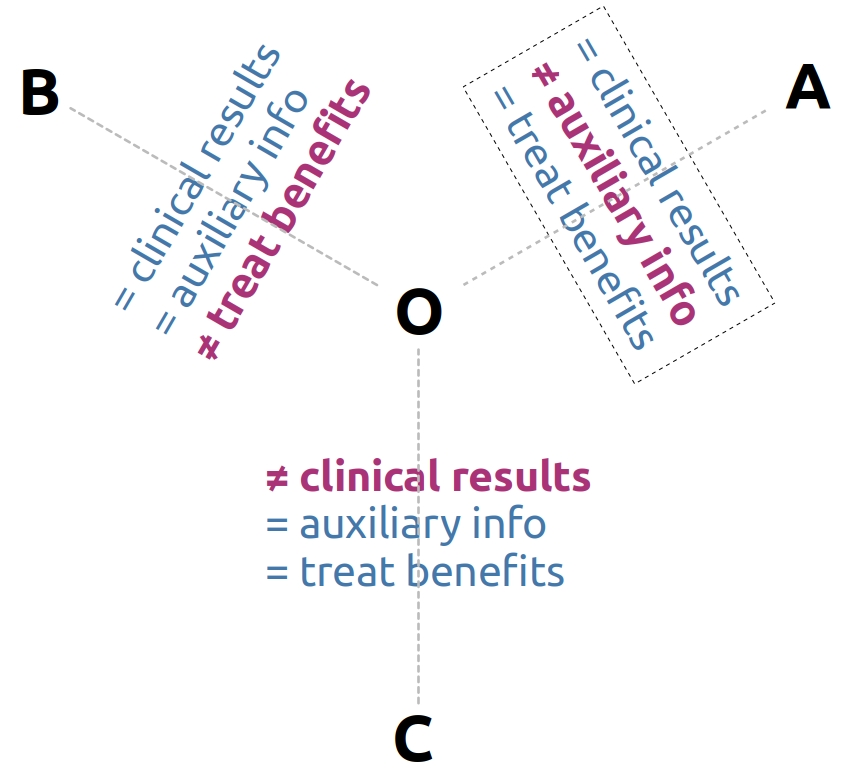
\includegraphics[width=\linewidth]{OABC.png}%
\vspace{-2em}% \caption{\mynotep{draft, needs better font sizes}}\label{fig:OABC}
\end{wrapfigure}
described there apply more generally to most, if not all, clinical problems of prognosis and treatment. These differences can be broadly categorized as \enquote{difference in auxiliary and background information} (Olivia and Ariel), \enquote{difference in benefit and availability of treatments} (Olivia and Bianca), \enquote{difference in clinical predictors} (Olivia and Curtis), as schematized in the side figure. Each of these difference categories can affect the clinician's final choice of optimal treatment. An assistive algorithm should therefore reflect these differences in its input, its output, or both:
\begin{itemize}
\item In principle there could be three kinds of input \enquote{slots}, where the clinician can input the current patient's specific values as regards clinical predictors, auxiliary information, and treatment options \amp\ benefits.
\item If input slots are only available for one or two of the categories above, the output should at least be of such a kind as to allow the clinician to integrate the current patient's specific values of the missing input categories.
\end{itemize}

To appreciate these requirements, contrast the input and output of many kinds of machine-learning classification algorithms. These typically only allow the input of a patient's clinical predictors, with no space for patient-specific auxiliary information or for adjustments of differences in background statistics (think of Olivia and Ariel). And they typically output only a discrete prognostic label (say, \enquote{stable \mci} vs \enquote{conversion to \ad}), but no measure of the uncertainty about that label. Unfortunately, such output does not allow the clinician to assess treatment benefits and losses for the current patient, for this assessment depends not on the presence (present or future) of a disease, but on the \emph{risk} of its presence. We shall discuss these points at length in \sects~\ref{sec:population_step} and~\ref{sec:utilities_step}.

\medskip

The purpose of the present work is to present an assistive algorithm that meets the requirements above. This algorithm is designed to first learn from a dataset of clinical data with relevant predictors and predictand%
%%%% Note on "predictand"
%
% The quantity that we want to forecast is in various texts called "dependent variable" or "response variable". I personally don't like either. Both can be misleading. Surely AD-conversion is not "dependent" on cognitive variates, for example. Moreover we'll see that we are actually swapping the role of "independent" and "dependent" variables in this work. Same goes for "response". With a readership of medical scientists it's best to avoid the special connotations of these words, leaving them for variables that are indeed biologically dependent.
%
% This leaves us with "predictand", literally "what has to be predicted", which is exactly what AD-conversion is. This term is used in climate science and meteorology. It's good because it does not misleadingly imply that AD-conversion biologically depends or is a consequence of other variables.
%%%%
\footnote{literally \enquote{quantity to be predicted} (\cf\ \emph{measurand} in metrology, \citealt[2.3]{jcgm1997_r2012}). We find this term, used in meteorology and climate science, more precise and less obscure or misleading than \enquote{dependent variate}, \enquote{response variate}, or similar.}, and then assist a clinician in the assessment of prognosis \amp\ treatment for new patients. It offers these ten features:
\begin{enumerate}
\item\label{item:feat_variates} It can work with clinical predictors comprising any combination of categorical and one-dimensional (continuous, discrete ordinal, unbounded or bounded, uncensored or censored) variates. The predictand can also be any combination of categorical and one-dimensional variates.

\item\label{item:feat_indifferentvariates} It treats predictor and predictand variates on equal footing, in the sense that the clinician can at any moment decide to predict some other variate given the rest.

\item\label{item:feat_conditionalstats} It does not require that the current patient be considered in all respects as a member of the population underlying the learning dataset. The patient can be considered a member only conditionally on particular variate values.
  
\item\label{item:feat_inputs} It accepts three inputs:
  \begin{enumerate}
  \item\label{item:input_predictors} the clinical-predictor values for the current patient;
  \item\label{item:input_aux} information about which predictand-predictor relationships learned from the dataset can be generalized to the current patient, and a prior prognostic probability representing auxiliary information;
  \item\label{item:input_treats} a set of treatment options and their benefits and losses for the current patient.
  \end{enumerate}

\item\label{item:feat_outputs} It yields three basic outputs
  \begin{enumerate}
  \item\label{item:ouput_predictors} any prognostic probabilities or likelihoods about predictors and predictand desired by the clinician, given input~\ref{item:input_predictors};
  \item\label{item:output_aux} final prognostic probabilities, given inputs~\ref{item:input_predictors}--\ref{item:input_aux};
  \item\label{item:output_treats} optimal treatment, given inputs~\ref{item:input_predictors}--\ref{item:input_treats};
  \end{enumerate}
  
\item\label{item:feat_modular_inout} Its input and outputs are modular, in the sense that the clinician can, for instance, give inputs~\ref{item:input_predictors}--\ref{item:input_aux} only, get a prognostic probability~\ref{item:output_aux} as output, and then proceed to treatment assessment by other means or algorithms.

\item\label{item:feat_imputation} It works even if predictor data are missing, both in the learning dataset and for the current patient.

\item\label{item:feat_uncertainty} It can quantify the uncertainty of its own outputs and therefore allow for sensitivity analyses. For example, it can tell how much a prognostic probability could have been different if the learning dataset had been larger, or whether the optimal treatment could be different if a particular missing predictor for the current patient had been available.

\item\label{item:feat_forecast} It can make various kinds of long-term forecasts, such as frequency of prognoses having given probabilities, frequency of prescribed treatments, and similar -- provided that the dataset used for its learning can be considered representative of the full population,

\item\label{item:feat_unbeatable} It is model-free and extracts the maximal amount of information theoretically contained in the learning dataset, and therefore achieves the maximal prognostic power that the predictors can yield. In other words, it is unbeatable.

\end{enumerate}

Let us comment on some of these features. We believe that the capability of working with complex predictands, feature~\ref{item:feat_variates}, is important for a more realistic and nuanced approach to prognosis. In the case of \ad, for instance, it is clear that a simple dichotomy \enquote{has disease} vs. \enquote{doesn't have disease} is an oversimplification \mynotep{more text and references?}. Without the capability of being used with patients having peculiar contexts or clinical situations, feature~\ref{item:feat_conditionalstats}, the algorithm would be of no use in the often occurring case of patients having special clinical contexts. The capability of dealing with missing data, feature~\ref{item:feat_imputation}, is important for a concrete implementation in a clinical setting, typically afflicted by imputation problems. Feature~\ref{item:feat_uncertainty} is extremely important for a clinician to assess the reliability of final decisions and inform the patient of the possibility of unwanted outcomes. Finally, features~\ref{item:feat_indifferentvariates} and~\ref{item:feat_unbeatable}, the fact that this algorithm yields the maximal amount of information (as determined by information theory) jointly contained in all variates, makes it valuable in general clinical research. The algorithm can, for example, forecast the maximal accuracy obtainable by \emph{any} inference algorithm based on the same predictors or another set of predictors; it itself attains that maximal accuracy.

Further features relevant for Machine Learning are given in \sect\mynotep{***}.

We call this algorithm a \emph{\ljm}, for reasons explained in the next section. It is at the moment available as a collection of scripts\footnote{\url{https://github.com/pglpm/ledley-jaynes\_machine}} in the R programming language \citep{rcoreteam1995_r2023}, which we plan to soon assemble into a clinician-friendly R package.

The next section~\ref{sec:the_machine} gives an intuitive understanding of the \ljm's underlying principles and workings. It is largely independent of the subsequent sections, so it can be skipped by readers who want to immediately see its application. Application is shown in \sect~\ref{sec:application}, using the four-patient fictitious scenario of \sect~\ref{sec:four_patients} as a concrete example; the final subsection~\ref{sec:additional_results} discusses applications to general medical research. A summary and discussion is given in \sect~\ref{sec:discussion}.

Mathematical details and proofs on which the present work is grounded are given in a companion technical note\footnote{\url{https://github.com/pglpm/ledley-jaynes\_machine/raw/main/ledley-jaynes\_machine.pdf}}, which explains more in detail how to use the R~scripts.

\bigskip% Newpage break just to help while writing the draft
\section{The \ljm}
\label{sec:the_machine}

This section can be skipped by % practitioners of Hearsay Science
readers not interested in the principles and mathematical details underlying the \ljm.

\subsection{Underlying theory and characteristics}
\label{sec:the_machine_principles}

The method to solve clinical decision-making problems such as the one of \sect~\ref{sec:intro} %, taking into account individual differences among patients,
is none other than Decision Theory: the combination of probability theory and utility theory. It integrates available clinical statistical data with each patient's unique combination of clinical results, auxiliary information, and treatment benefits, in a mathematical framework, completely determined by basic self-consistency requirements.\footnote{\citet[\chaps~13--14]{jaynes1994_r2003,vonneumannetal1944_r1955,cox1946,savage1954_r1972,luceetal1957,raiffaetal1961_r2000,raiffa1968_r1970,lindley1971_r1988,kreps1988}.}

Medicine has the distinction of having been one of the first fields to adopt Decision Theory, with the pioneering work by Ledley and Lusted \citeyearpar{ledleyetal1959,ledleyetal1959b,ledleyetal1960,lustedetal1960}, who also promoted its algorithmic implementation \citep[see especially \sect~1-5 p.~21]{ledley1959,ledley1960}. Clinical decision-making is today explained and exemplified in brilliant textbooks for medical students and clinicians \citep{weinsteinetal1980,soxetal1988_r2013,huninketal2001_r2014}. An outline is given in \sect~\ref{sec:expected_utility_theory}.

The \enquote{\ljm} is an algorithmic implementation of the main calculations underlying the clinical decision-making process, as dreamed by Ledley and Lusted: from the comparison of a patient's specific predictors with the statistics offered by a clinical database, to the choice of optimal treatment. The name is a homage to Ledley -- who, incidentally, died of \ad\ \citep{shahetal2013} -- and to Jaynes \citeyearpar{jaynes1994_r2003}, who brilliantly explained the inductive logic underlying such a \enquote{robot}.


Decision theory is also the normative foundation for the construction of an Artificial Intelligence agent capable of rational inference and decision making \citetext{\citealt[part~IV]{russelletal1995_r2022}; \citealt[\chaps~1--2, 13--14]{jaynes1994_r2003}}. The \ljm\ can therefore be seen as an \emph{ideal} machine-learning algorithm. It is \enquote{ideal} in the sense of being free from special modelling assumptions (this is why we do not call it a \enquote{model}) and from limitations of its informational output, characteristic of most common machine-learning algorithms; not \enquote{ideal} in the sense of being impracticable. Quite the opposite, the present work shows that this ideal machine-learning algorithm can today be applied at insubstantial computational cost. % It is preferable to popular algorithms such as neural networks, random forests, support-vector machines, which are unsuited to clinical decision-making problems owing to their input and output limitations and underlying special assumptions. We discuss this matter further in \sect~\ref{sec:discussion}.

More concretely, the \ljm\ is ideal because \emph{it computes the probability distribution over all possible long-run joint frequency distributions from which the learning dataset can originate} (joint distributions for all predictor and predictand variates). This is the maximum possible amount of information that can be extracted from the learning dataset, in a strict information-theoretic sense. From this probability distribution, the \ljm\ can indeed calculate any quantity outputted by other machine-learning algorithms. For example \citep[for terminology see \eg][\sect~8.6]{murphy2012}:
\begin{itemize}
\item \emph{\enquote{Discriminative} algorithms:} the probability $\p(Y \| X)$ of any set of predictands $Y$ given any set of input predictors $X$.

\item \emph{\enquote{Generative} algorithms:}  the probability $\p(X \| Y)$ of any set of input predictors $X$ given any set of predictand values $Y$.

  More generally, the machine can compute any joint, marginal, or conditional probabilities $p(Z',Z'')$, $p(Z')$, $p(Z'\|Z'')$ for any desired subsets of variates $Z', Z''$.

\item \emph{Regression or classification:} the average value of any set of variates $Y$, given any other set of variates $X$, including the special case of predictand $Y$ and predictors $X$. The uncertainty or variability around such an average is also automatically computed.
  
\item \emph{Functional regression:} if the predictand $Y$ or any other variate of interest turns out to be a function $f$ of variates $X$, then their conditional probability will be a delta distribution: $\p(Y\|X) = \delt[Y-f(X)]$.
  % We must remember that a function can always be represented by a probability distribution, but not vice versa.\footnote{The function $f\colon x \mapsto y=f(x)$ corresponds to the probability density $\p(y\|x) = \delt[y-f(x)]$, where $\delt$ is a delta distribution.}
  Thus the \ljm\ always recovers a functional relationship if there is one, as well as its noise distribution.
\end{itemize}
Furthermore, the machine also quantifies the uncertainty of all outputs above. More precisely, it takes into account that the statistical properties of the learning dataset could be different from those of its original population, owing to sampling fluctuations; and it computes how much any of the outputs above would probably change if more learning data were collected.

In the next section, we explain intuitively how the \ljm\ computes the general probability distribution over long-run frequencies; but we can already summarize a couple of special characteristics brought about by such computation. Unlike machine-learning algorithms such as neural networks, random forests, support-vector machines, logistic regression, or generalized linear models, the \ljm\ does not do an optimization during the learning phase, searching for the minimum of some objective function. It does a full \emph{hypothesis-space survey}. % Inference and generalization in fact essentially rely on averaging operations in problems such as the present one \citetext{\citealt{definetti1930,definetti1937,dawid2013}; \citealt[\sects~4.2--4.3]{bernardoetal1994_r2000}}
The optimization done by most machine-learning algorithms is an approximate form of this survey, based on the assumption or hope that the most relevant portion of the hypothesis space will be around the extremum \citetext{\citealp[\chap~16]{mackay1992,murphy2012}; \citealp[see also][]{selfetal1987}}. The underlying necessity of a more extensive survey, however, becomes manifest in many of the obligatory procedures that go together with the training of most machine-learning algorithms, cross-validation being a prominent example \citep{mackay1992b}. This leads to another special characteristic: the \ljm\ does not need validation sets, test sets, or other data splits; nor does it need cross-validation procedures. Intuitively this is the case because the underlying hypothesis-space survey realizes a sort of full-fledged cross-validation and data partition. It can indeed be proved that one of the internal computations of the machine is mathematically equivalent to doing $k$-fold cross-validations for \emph{all possible} data splits and $k$ \citep{portamana2019b,fongetal2020}.

Such flexibility and informationally rich output come, of course, at a computational cost. Until some years ago, the cost would have been prohibitive in all but the simplest inferential problems. But today, an inference problem involving 13 variates and 700 datapoints, such as the example considered in the present work, takes less than six hours of computation on an office computer workstation. We discuss computational limitations further in \sect~\ref{sec:rangeLJM}.

\subsection{Intuitive understanding of the learning algorithm}
\label{sec:the_machine_learning}

The calculations by which the \ljm\ learns and operates are univocally determined by Cox's theorem \footnote{\citealp{cox1946,cox1961,polya1954,polya1954b_r1968,tribus1969,fine1973,rosenkrantz1977,paris1994_r2006,snow1998,arnborgetal2001,snow2001,claytonetal2017}; for a review see \citealp{vanhorn2003}.}, which determines quantitative inference rules from self-consistency requirements, and by de~Finetti's theorem\footnote{\citealp[\sects~4.2--4.3]{definetti1930,definetti1937,bernardoetal1994_r2000}; for a review see \citealp{dawid2013}.}, which further constrains these rules in the case of \enquote{generalization from similar cases}. These calculations have a very intuitive interpretation.

We consider a patient to be a member of some population of similar past, present, and future patients. Suppose we knew the joint frequency distribution of all possible combinations of predictor and predictand values in such a population. We would then judge the probability for a patient's particular variate values to be equal to their corresponding population frequency. Pure symmetry considerations lead to this result \citep[\sects~4.2--4.3]{definetti1930,dawid2013,bernardoetal1994_r2000}. The same would be true for conditional and marginal probabilities and frequencies.\footnote{If there were a functional relationship from predictors to predictand, then the predictand value corresponding to the function output would have conditional frequency and probability equal to 1, and all other values to 0. Therefore, this point of view still encompasses a functional relationship as a particular case.} This population frequency distribution would bound the maximal prognostic power attainable with the given predictors in the population. A higher prognostic power could only be attainable by using additional or different predictors having sharper conditional frequencies for the predictand in the population. Given knowledge of such frequency distribution, there would be no problem of \enquote{generalizing} to new patients, because each new patient would already be counted in the known frequencies. An inference algorithm would only need to enumerate and memorize, rather than to learn and generalize.

Learning and generalization come into play because the frequency distribution for the population is unknown: we only have a sample from it, the \enquote{learning dataset}. Thus we can, at most, assign a probability to each possible frequency distribution. This is precisely what the \ljm\ does.

The way in which the machine assigns a probability to each \enquote{candidate} true frequency distribution is also intuitive. It combines two factors: (i) how well the candidate fits the sample dataset, (ii) how biologically or physically reasonable the candidate is. The first factor is easily computed: it is the joint probability of the dataset if it were sampled from a population having that candidate frequency. The second factor is a prior probability expressing how reasonable that candidate is.\footnote{It must be emphasized that some notion of \enquote{reasonable candidate} is unavoidable and clearly present in the construction or testing of any inference algorithm. How can we otherwise judge that an algorithm is over- or under-fitting? Such judgement implies that we have a preconceived, reasonable reference distribution in the back of our minds. The fit is either intuitively compared with the preconceived reference; or is compared with a known, ground-truth test for testing owing to its similarity with the preconceived reference.} The most general natural requirement for \enquote{reasonableness} is that the candidate should have some degree of smoothness, owing to physical and biological reasons. Figure~\ref{fig:prior_distribution} shows samples of what the machine considers to be \enquote{reasonable candidates} for the population frequency distribution of a discrete variate. Note that no frequency distributions are excluded; they are only given higher or lower probabilities.
\begin{subfigure}[t]\setcounter{subfigure}{0}
  \centering%
  \begin{minipage}[c]{0.39\linewidth}\centering
    
\includegraphics[width=\linewidth]{priorexamples_AVDEL30MIN_neuro.pdf}
  \caption{Samples of initially probable candidates of the true population frequency distribution, for a variate such as \ravltdel\ %AVDEL30MIN\_neuro
    or \ravltrec. %AVDELTOT\_neuro
    }\label{fig:prior_distribution}
  \end{minipage}\hfill
  \begin{minipage}[c]{0.59\linewidth}\centering%
\makebox[0.49\linewidth]{\footnotesize dataset}%
\hfill%
\makebox[0.49\linewidth]{\footnotesize high-probability candidate}%
\\[-1em]
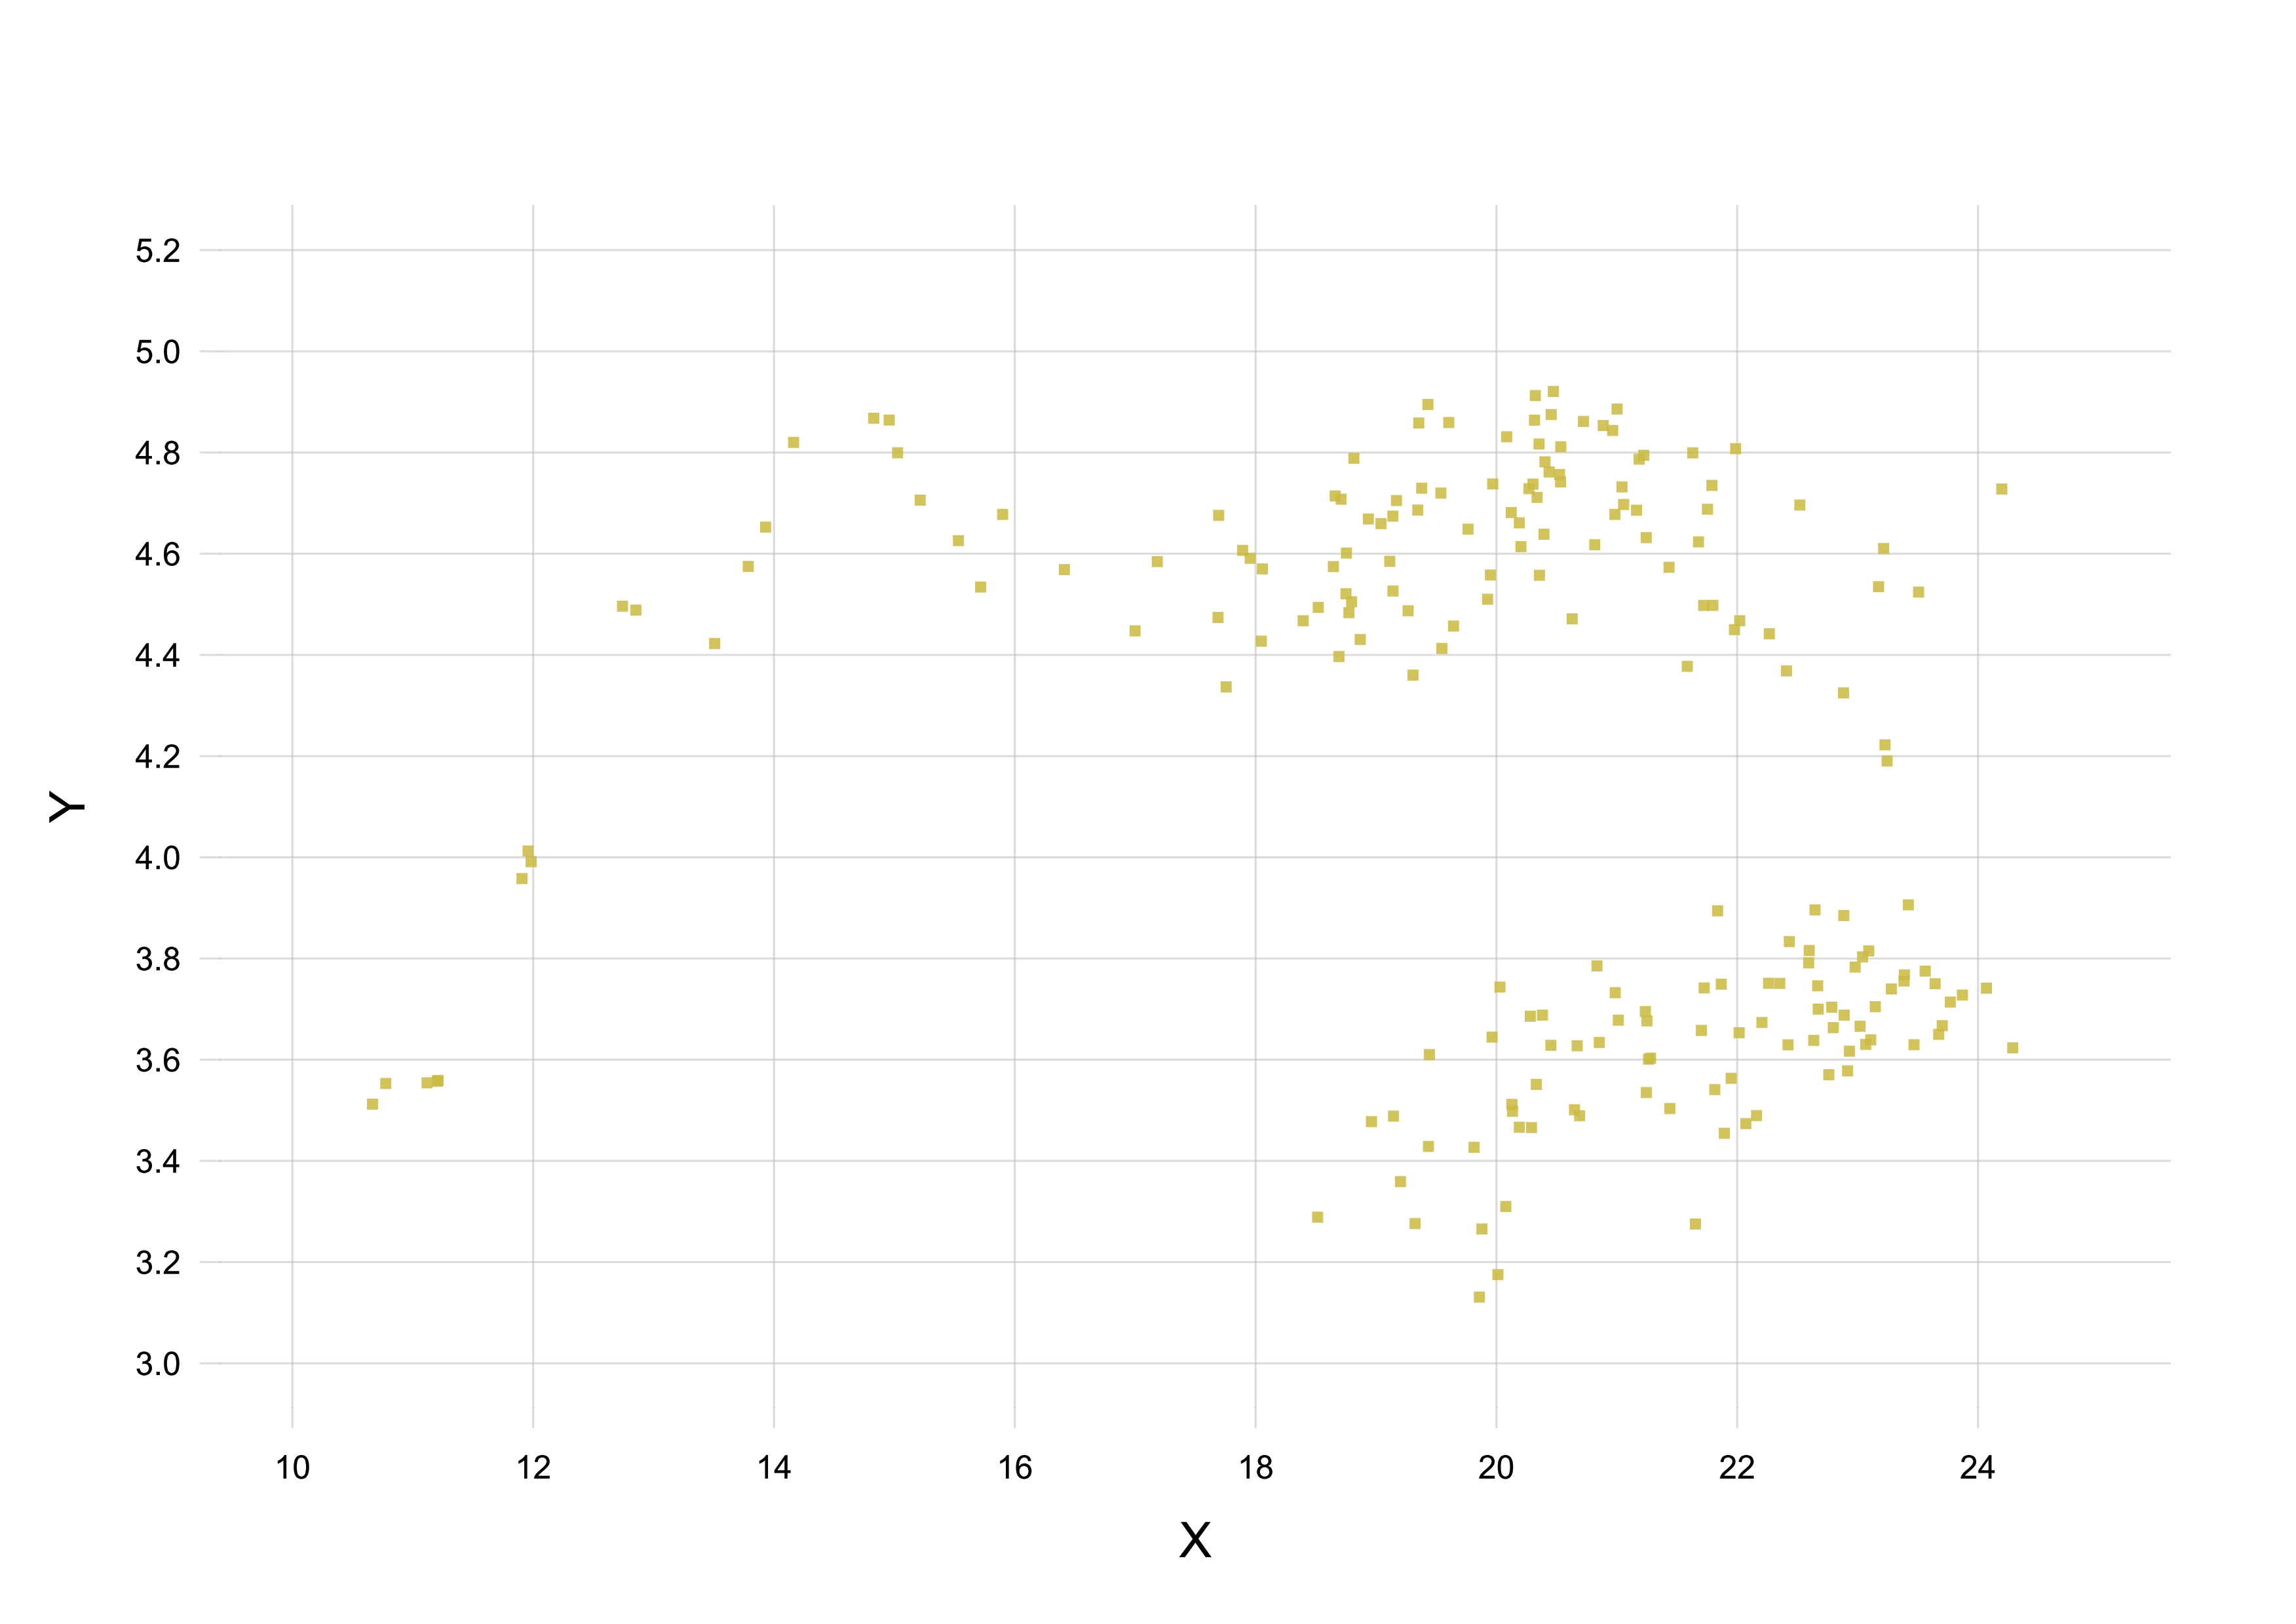
\includegraphics[width=0.49\linewidth]{exampledistr_sample_all.pdf}%
\hfill%
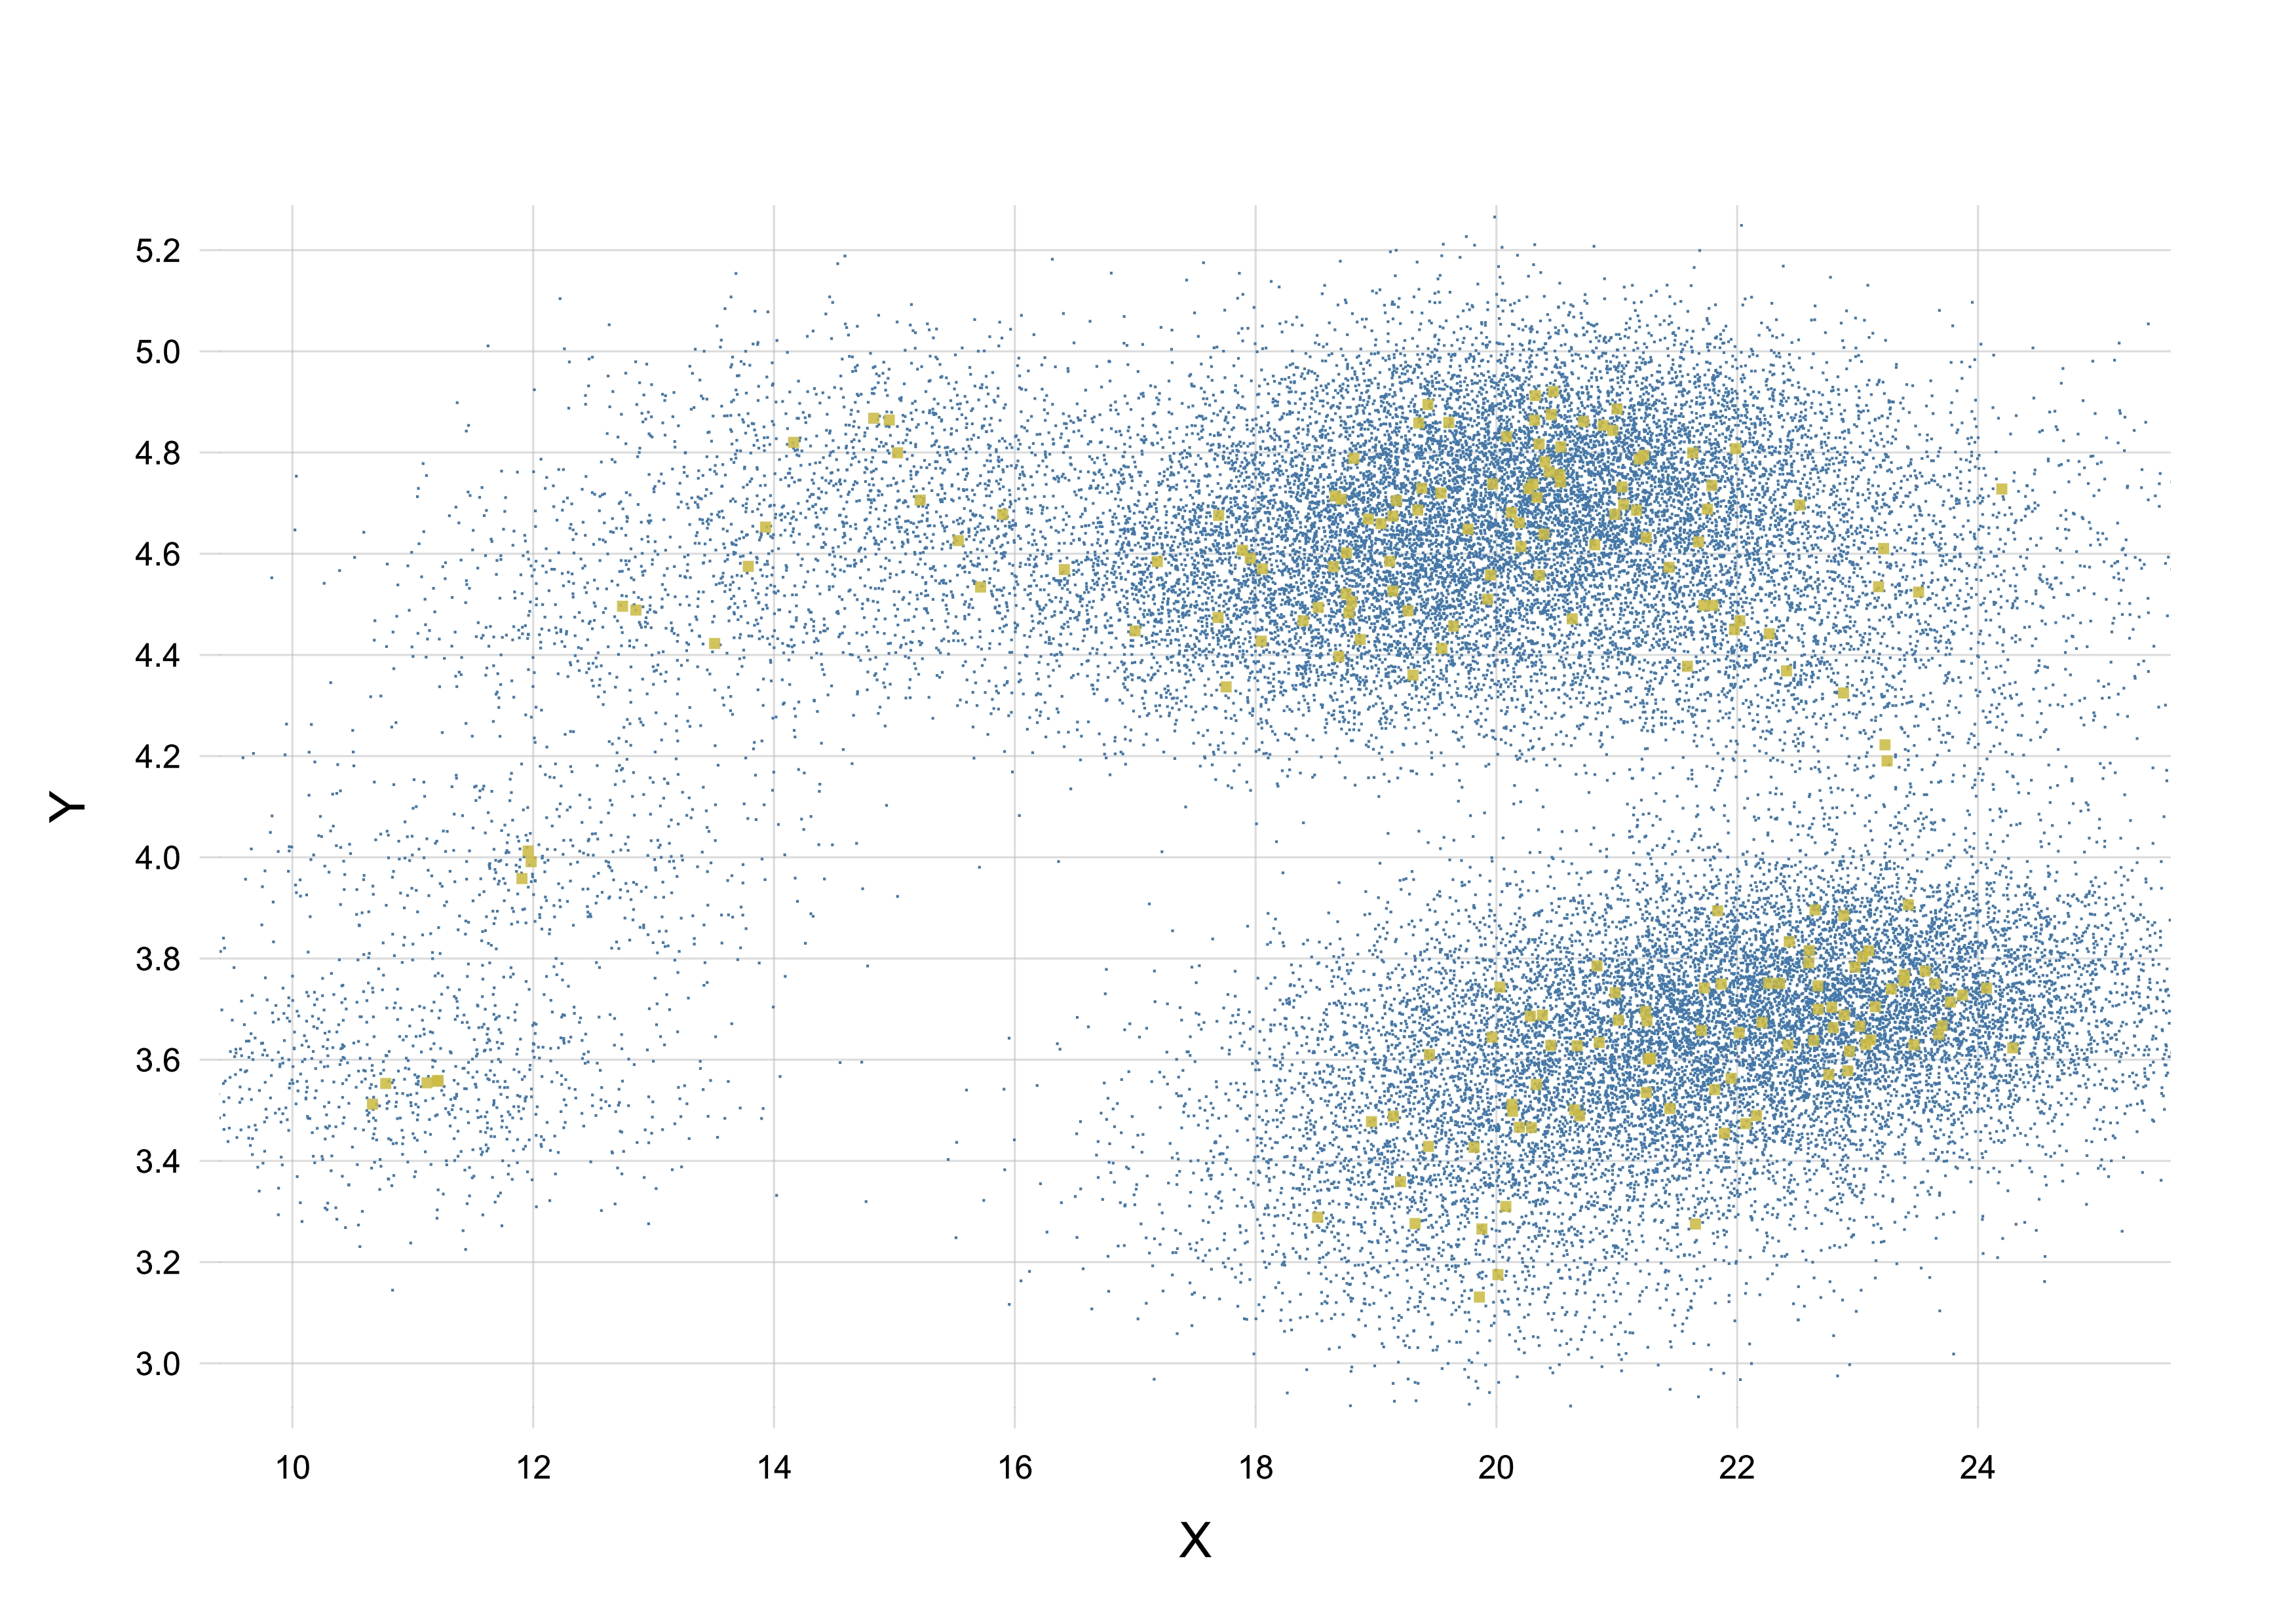
\includegraphics[width=0.49\linewidth]{exampledistr_okish_all.pdf}%
\\
\makebox[0.49\linewidth]{\footnotesize low-probability cand. (poor fit)}%
\hfill%
\makebox[0.49\linewidth]{\footnotesize low-probability cand. (unreasonable)}%
\\[-1em]
  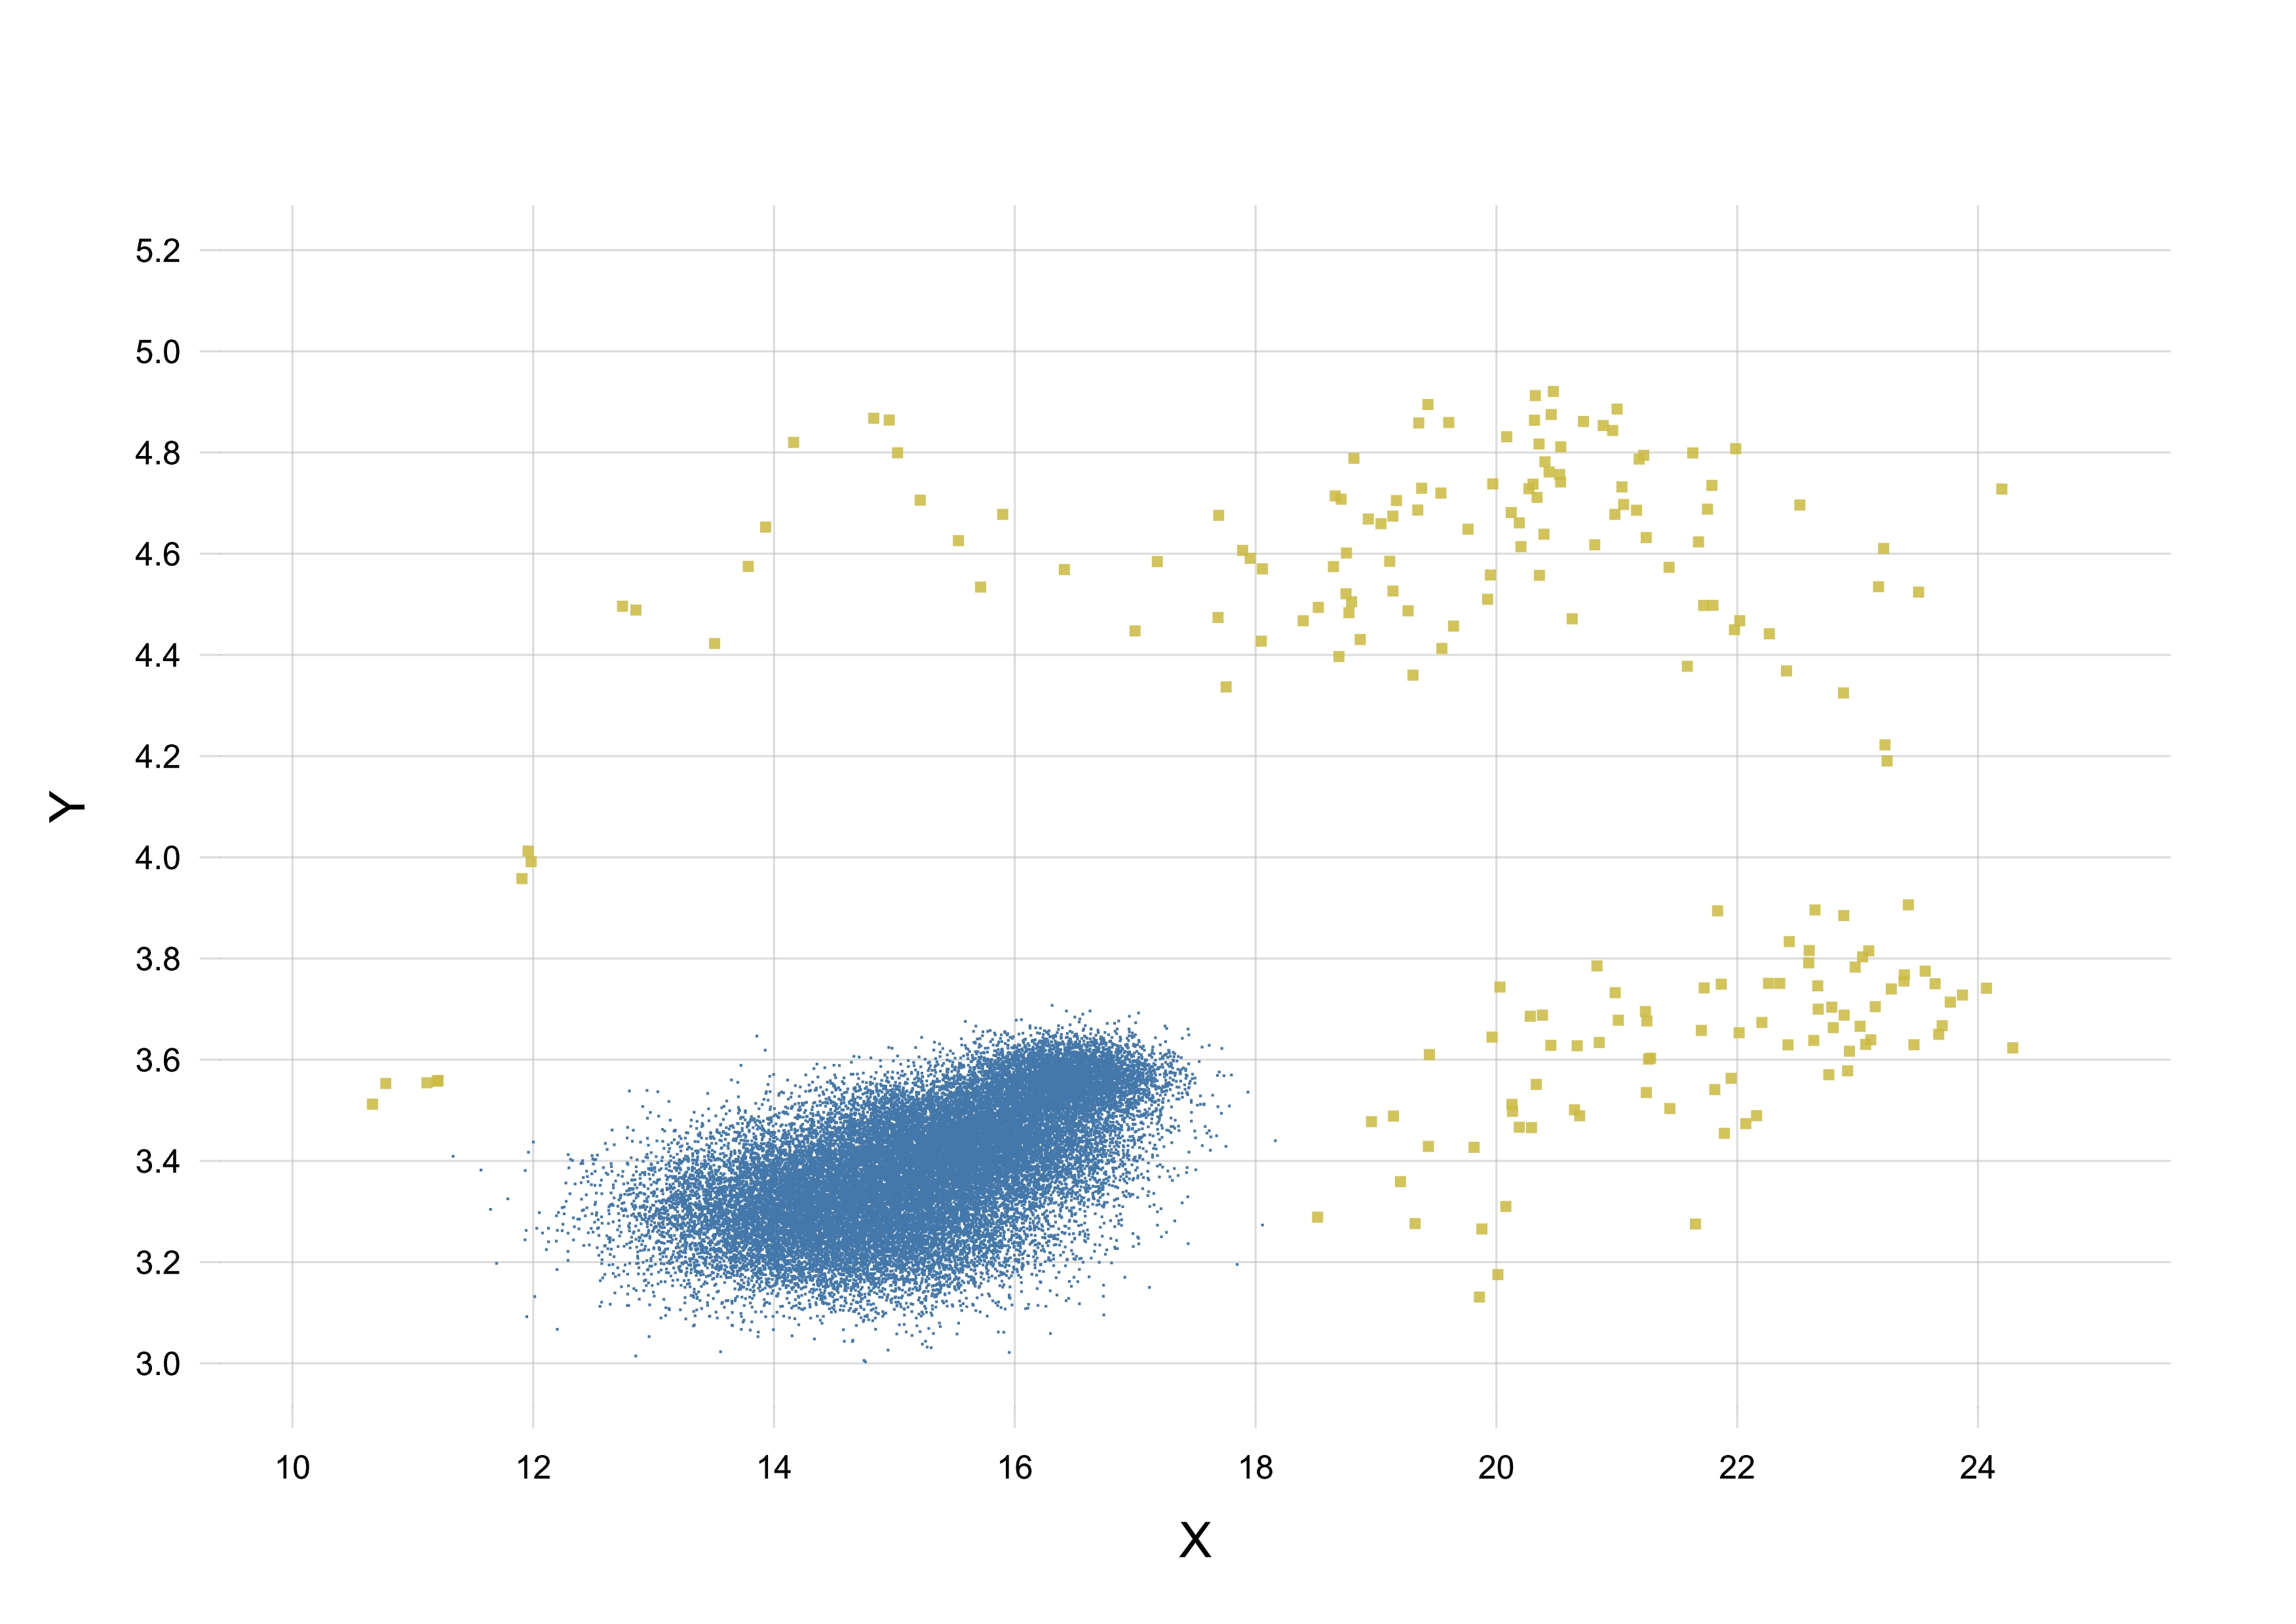
\includegraphics[width=0.49\linewidth]{exampledistr_unlikely_all.pdf}
  \hfill
  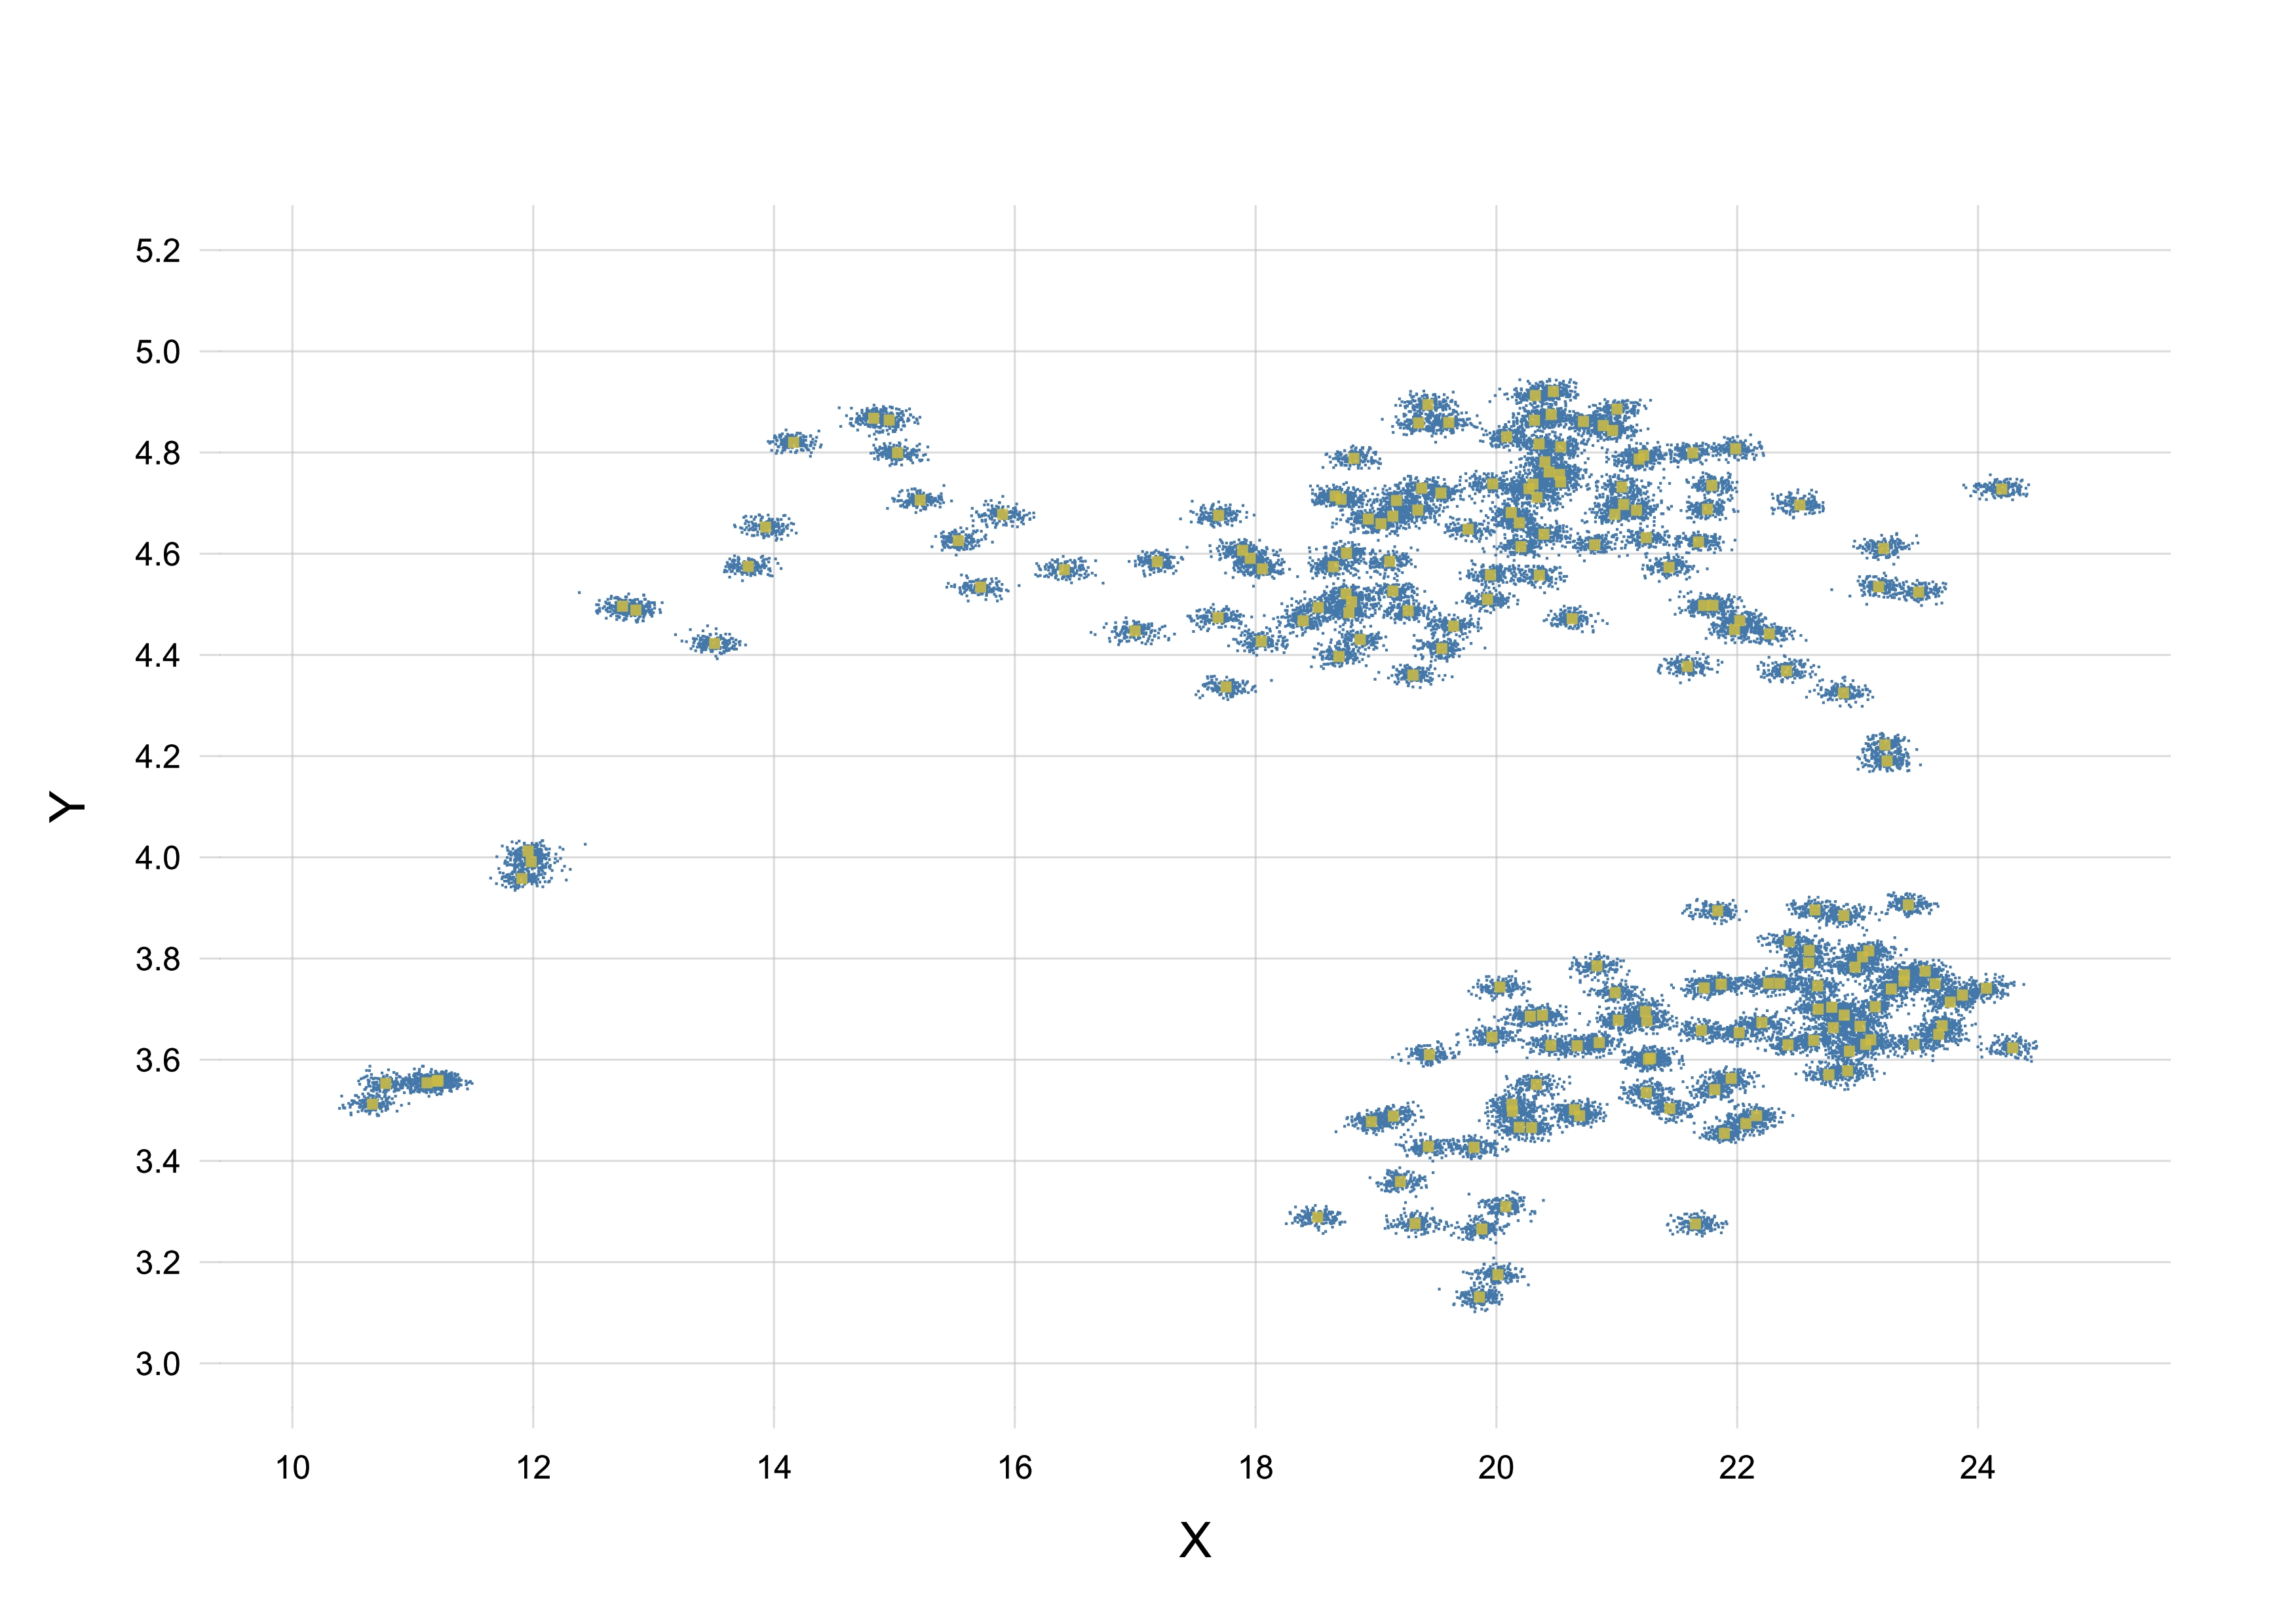
\includegraphics[width=0.49\linewidth]{exampledistr_strange_all.pdf}
  \caption{Illustration of the two factors determining the final probability of a candidate population frequency distribution. \emph{Upper-left}: an example dataset with two variates. \emph{Upper-right}: candidate frequency distribution with high final probability; it fits the data and is reasonable. \emph{Lower-left}: candidate distribution with low final probability; it is reasonable but does not fit the data. \emph{Lower-right}: candidate distribution with low final probability; it fits the data but is not reasonable.}\label{fig:inferring_distribution}
  \end{minipage}
\end{subfigure}%


The product of the two factors (i), (ii), normalized, yields the probability of each possible frequency distribution. An illustration of factors (i), (ii) at work is given in \fig~\ref{fig:inferring_distribution} for an example problem with two variates. The \ljm\ outputs the distribution of these final probabilities in the form of a large sample (the amount is decided by the user) drawn from it. In this form, all other marginal or conditional probabilities and averages of interest are calculated via Monte Carlo integration. This is the same methodology, but in nonparametric form, used in various inferences about the black holes M87 and Sagittarius~A\textsuperscript{*} \citep{eht2019,eht2022}.




\bigskip% Newpage break just to help while writing the draft
\section{Example application}
\label{sec:application}

\begin{table}[t]\centering
%  \begin{minipage}{0.75\linewidth}
    \begin{framed}
      \small
      \caption{\small\bf Main inferential and decision-making steps}\label{tab:main_steps}
      \begin{enumerate}\itemsep1em
        \setcounter{enumi}{-1}
      \item\label{item:learn} Find or build an appropriate dataset of clinical cases comprising values of the predictors and predictand of interest. Datapoints with partially missing values are allowed.

        Input the dataset into the \ljm\ and let it infer the joint full-population frequencies of predictors and predictand behind the dataset.

      \item\label{item:predictors} Measure the present patient's predictor values and input them in the \ljm. Partially missing values are allowed.

      \item\label{item:population} Assess which conditional statistics of the dataset can be applied to the present patient, and any auxiliary clinical information available. Quantify the latter it in a prior probability.

        Input the relevant statistics and auxiliary information for the present patient into the \ljm. 

        Upon request, the machine can now output the final probability of the predictand's true value for the patient, as well as any other probabilities and likelihoods of interest.
        
      \item\label{item:utilities} Assess the clinical courses of action (treatments, more tests, and so on) available for the present patient, and the utility (benefit and loss) of each course of action, depending on each possible predictand value for the patient.

        Input the patient's utilities into the \ljm. The machine outputs the course of action having maximal expected utility.

        Upon request, the machine can output the probability of gaining different utilities, perform sensitivity analyses for missing data, and do other similar tasks.
      \end{enumerate}
    \end{framed}
%  \end{minipage}
\end{table}

In this section, we illustrate how the \ljm\ is applied in the example case outlined in \sect~\ref{sec:four_patients}. Although the patients are fictitious, the dataset is real and briefly discussed in the next subsection. The main inferential and decision-making steps are summarized in table~\ref{tab:main_steps}. As mentioned in \sect~\ref{sec:intro_purposes}, steps 1.--3. are modular: the clinician is free to stop after any of them and use their output in other ways or with other algorithms.


These steps are illustrated in the next three subsections, preceded by an explanation of their rationale. They are presented in chronological order as the clinician would apply them. % In each section, a general overview and discussion of the theory and method behind the specific step is first given, followed by the concrete application to our example case.
Steps 1.--3. could also be presented in reverse order; which would be more suited to their logical dependence, as the procedure in each step is actually motivated by the one in the next. We suggest that readers familiar with the principles of clinical decision-making read the following subsections in \ref{sec:dataset}--\ref{sec:predictor_step}--\ref{sec:population_step}--\ref{sec:utilities_step} order; whereas readers unfamiliar with these principles read them in \ref{sec:dataset}--\ref{sec:utilities_step}--\ref{sec:population_step}--\ref{sec:predictor_step} order.


\setcounter{subsection}{-1}
\subsection{Predictors, predictand, and learning dataset}
\label{sec:dataset}

The dataset used in our example comes from the study by the Alzheimer's Disease Neuroimaging Initiative (\adni). This longitudinal multicentre study is designed to develop and validate neuroimaging and biochemical biomarkers for the early detection, monitoring, and treatment of \ad\ \citep{petersenetal2010}. The present dataset consists of 704 \adni\ subjects meeting the criteria for \mci\ at their first, baseline assessment who additionally had a minimum of two following, additional study visits, as well as three \textsc{mri} examinations. Each subject's diagnostic status was reevaluated at each study visit. This longitudinal diagnostic label is used as the predictand variate $\cad$ in our study: it categorizes each subject as either converting to \ad\ after the first study visit ($\cad=1$) or remaining stable with \mci\ ($\cad=0$). The dataset has 325 subjects (46.2\%) with $\cad=1$ and 379 (53.8\%) with $\cad=0$. Criteria used for classifying subjects as having \mci\ or \ad, as well as \adni's general criteria for subject inclusion, are described in \citet{mckhannetal1984,petersenetal2010}.


The 12 predictor variates consist of the results of eight tests for cognitive function (\anart, \cft, \gds, \ravltimm, \ravltdel, \ravltrec, \tmta, \tmtb), the presence of the \apoe-e4 risk allele \citep{liuetal2013}, a normalized measure of hippocampal volume (\hv), \age, and \sex. Further details about these variates and their selection can be found in \citet{ryeetal2022}. \mynotew{add details about specially sampled variates (age?), important for step~2.} The cognitive variates are integer-valued; hippocampal volume and age are continuous, and \apoe\ and sex are binary. The values of one or two of these predictors were missing for 30 subjects in the dataset.

The \ljm\ took less than five hours (on a 16-core Intel Core i9-12900K CPU) to calculate the probability distribution for the possible population joint frequencies distributions of the 13 variates. Some results can already be visualized after this inference.

Figure~\ref{fig:marginal_pop_distributions} shows, on the left, the predicted distributions of \ravltdel, \ravltimm, \gds, and hippocampal volume for the subpopulation of patients that will convert to \ad\ (red dashed) and the subpopulation that will remain with stable \mci\ (solid blue). On the right, the predicted frequency of conversion in the full population is given, conditional on the same predictors. The thin curves are 100 samples of highly probable frequency distributions; the thicker lines are their means, which are also the predictive conditional probabilities.
\begin{figure}[!t]
\centering%
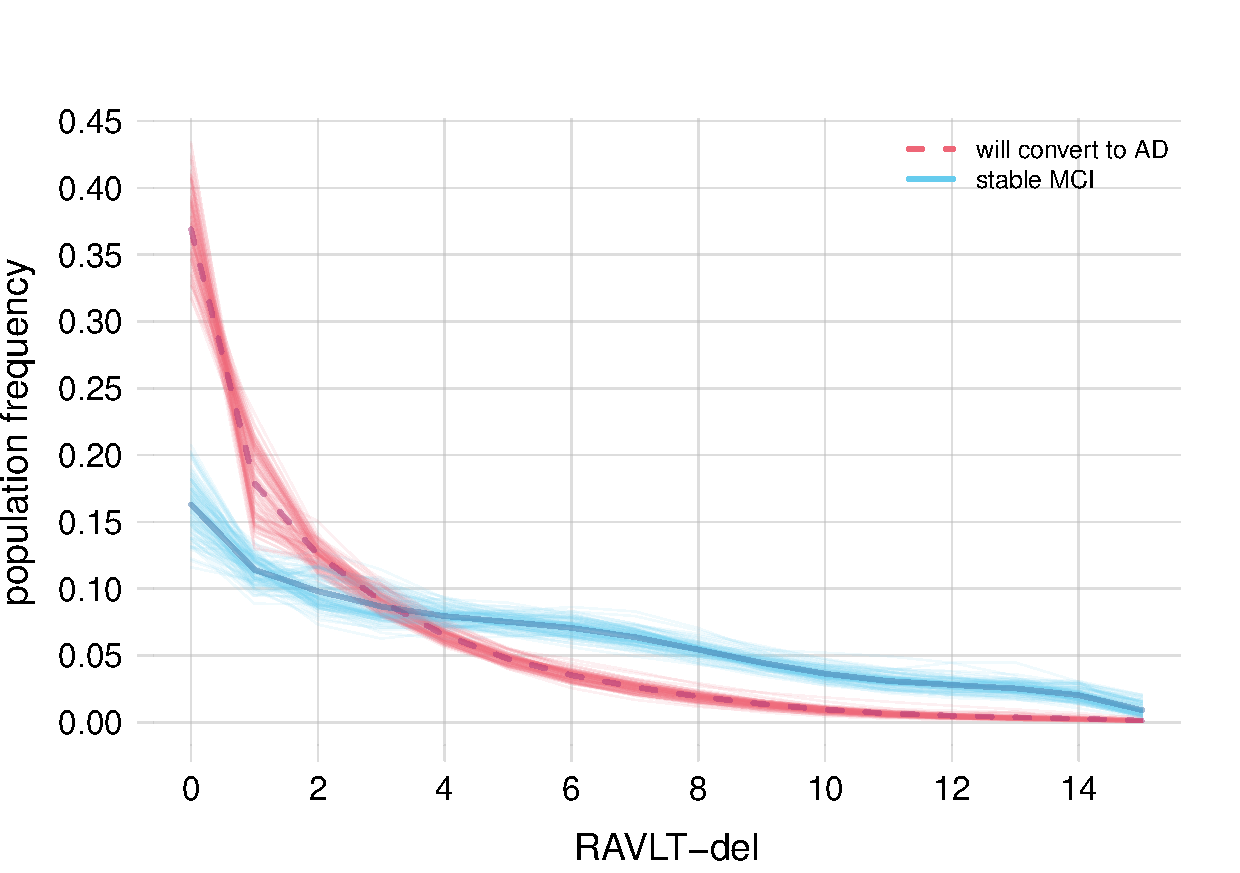
\includegraphics[width=0.43\linewidth]{population_distr_RAVLT-del.pdf}%
\qquad%
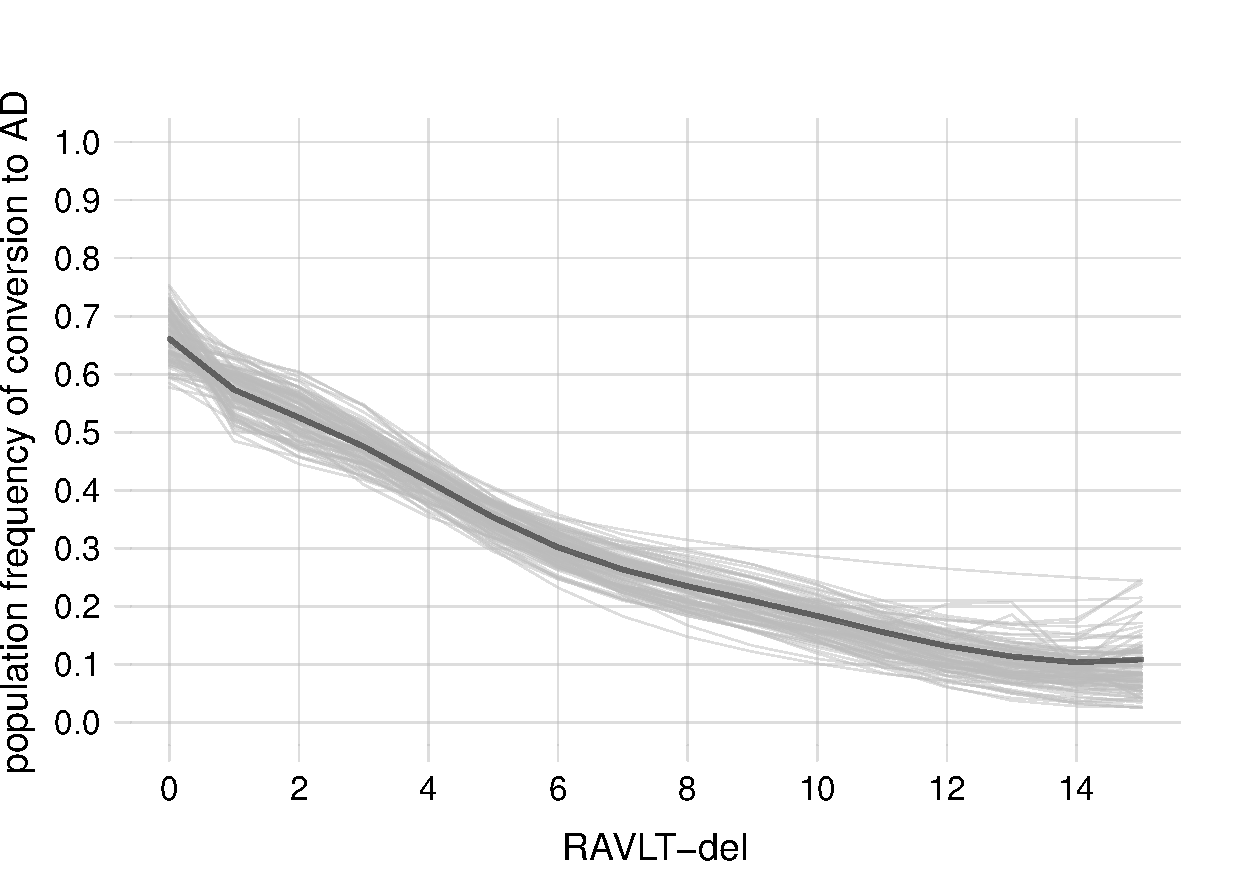
\includegraphics[width=0.43\linewidth]{prob_conversion_RAVLT-del.pdf}%
\\
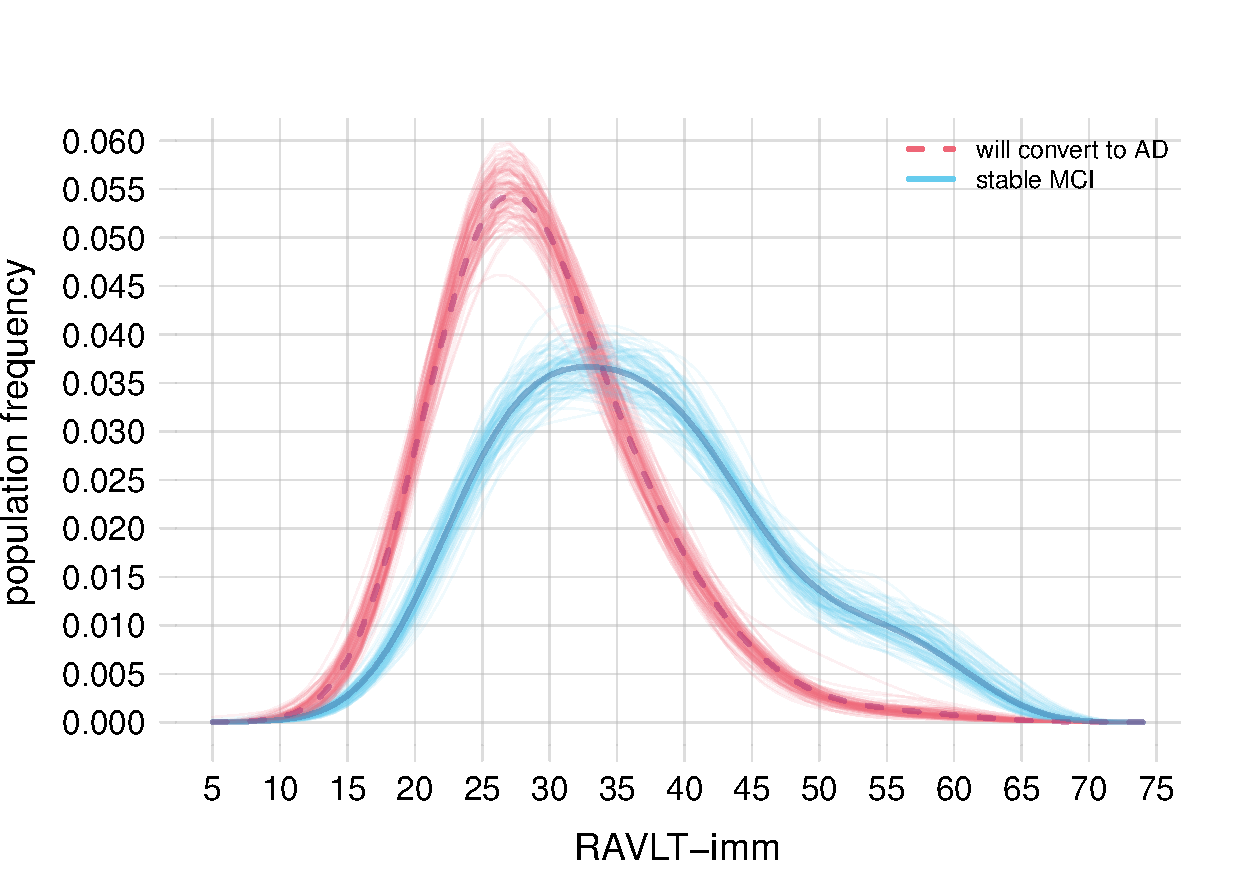
\includegraphics[width=0.43\linewidth]{population_distr_RAVLT-imm.pdf}%
\qquad%
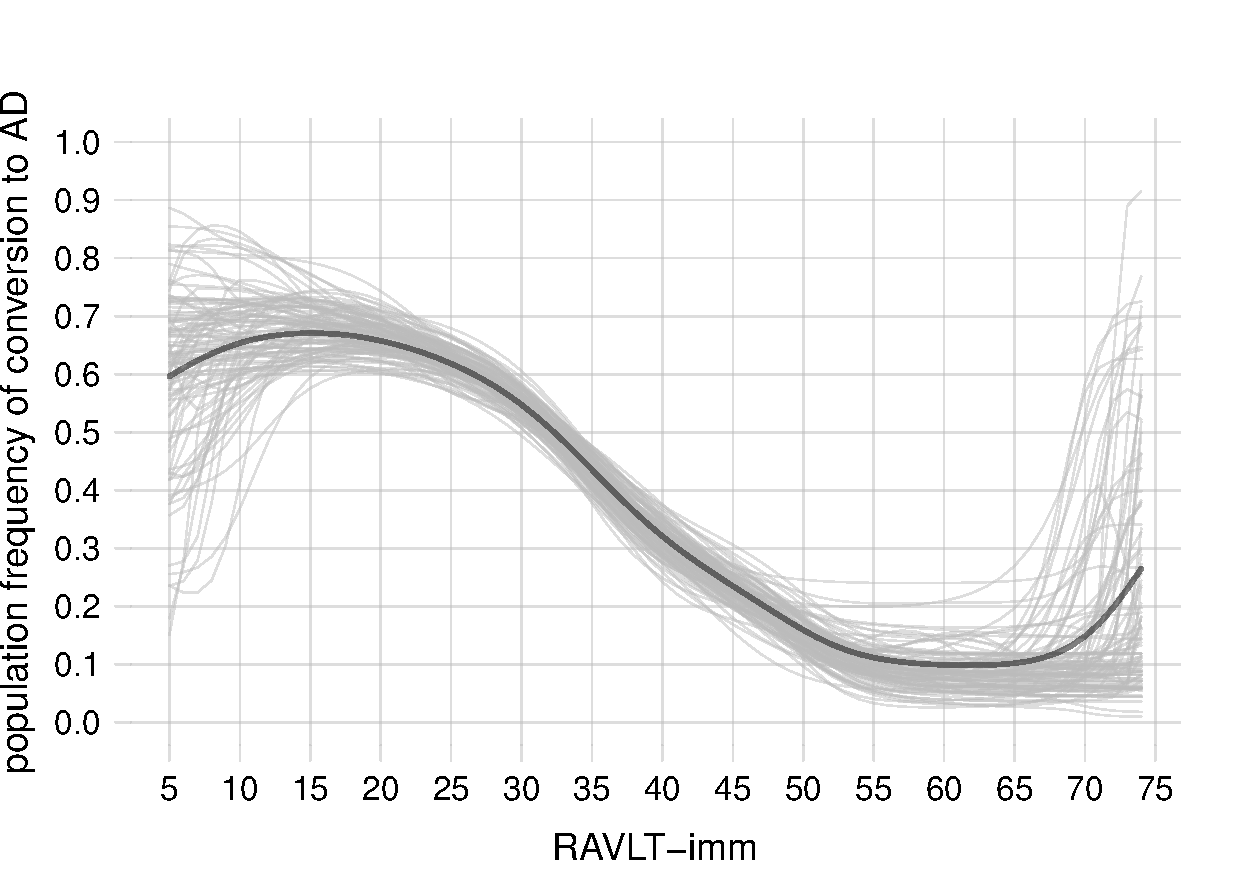
\includegraphics[width=0.43\linewidth]{prob_conversion_RAVLT-imm.pdf}%
\\
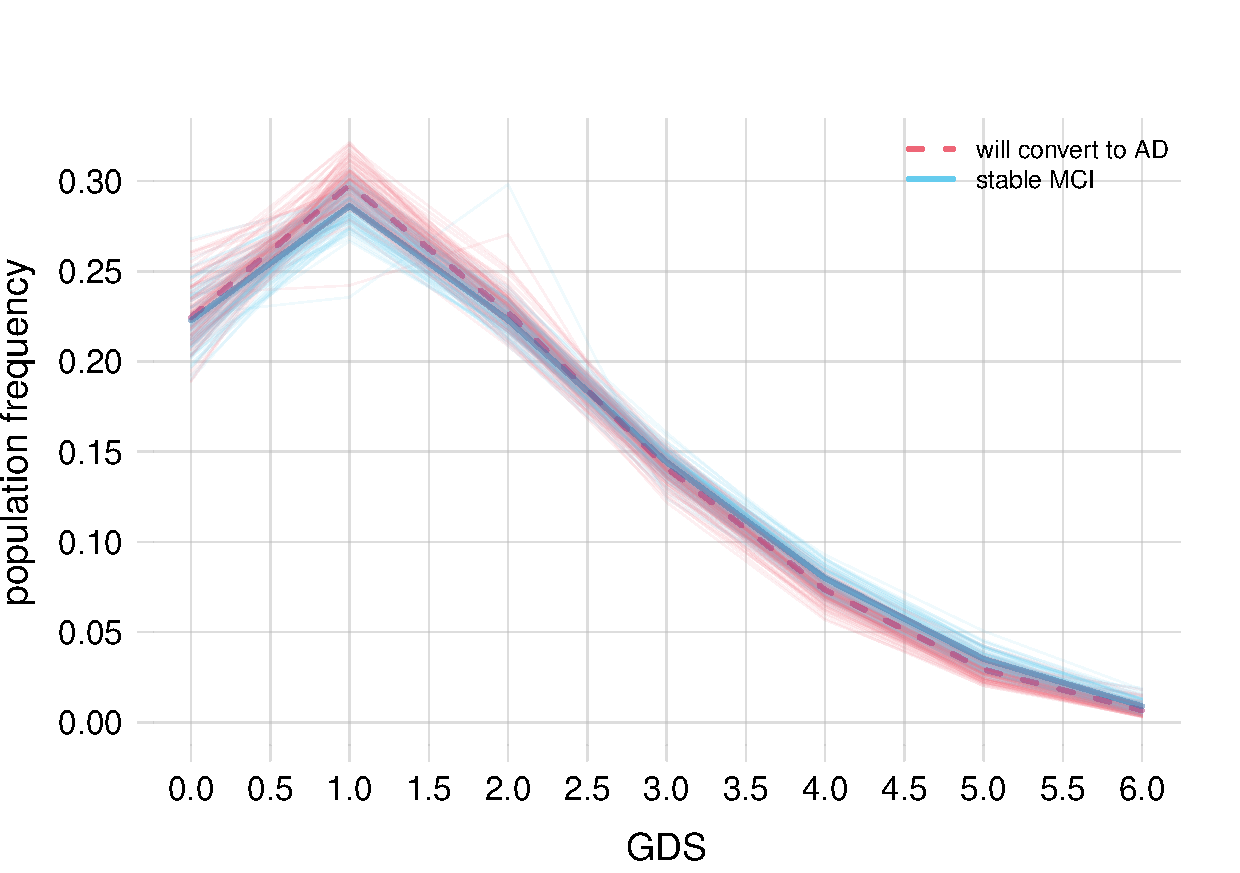
\includegraphics[width=0.43\linewidth]{population_distr_GDS.pdf}%
\qquad%
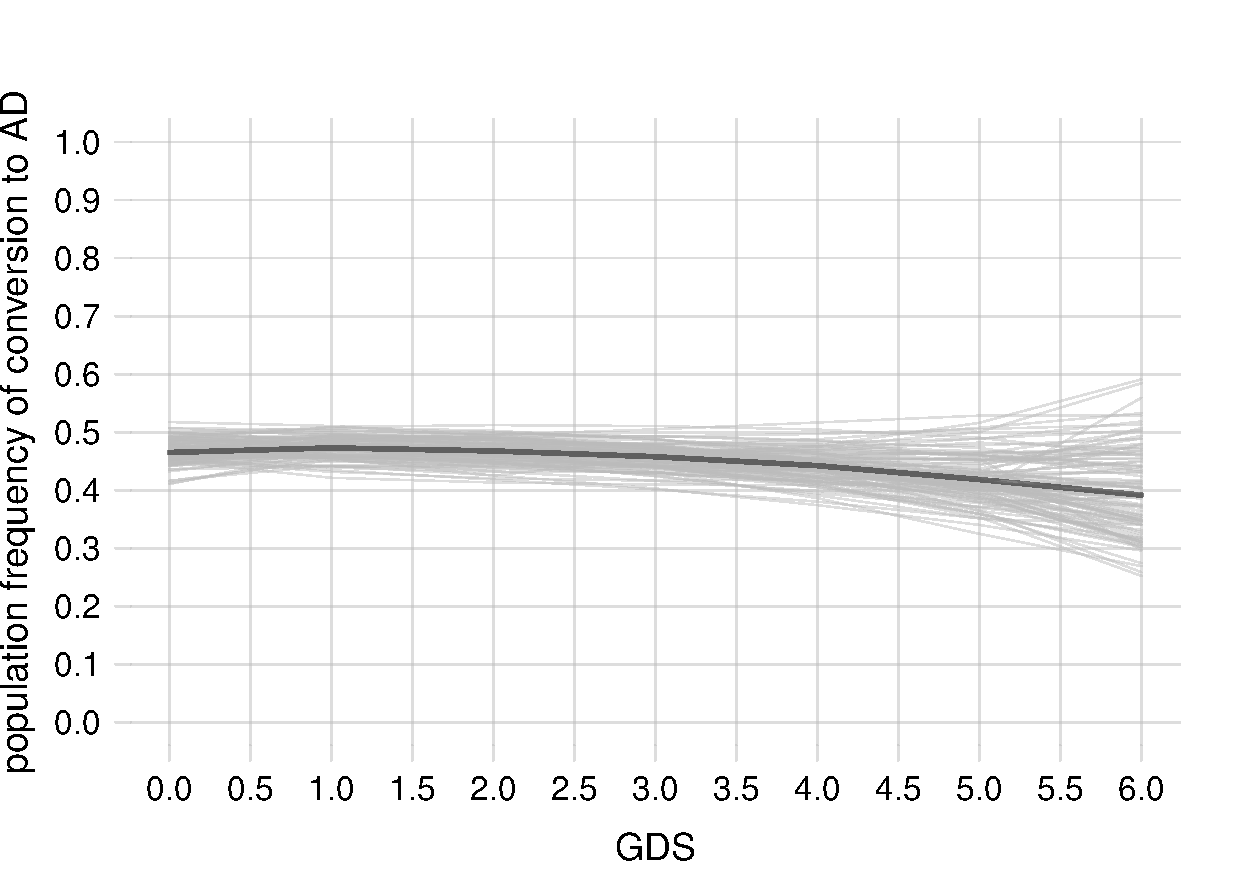
\includegraphics[width=0.43\linewidth]{prob_conversion_GDS.pdf}%
\\
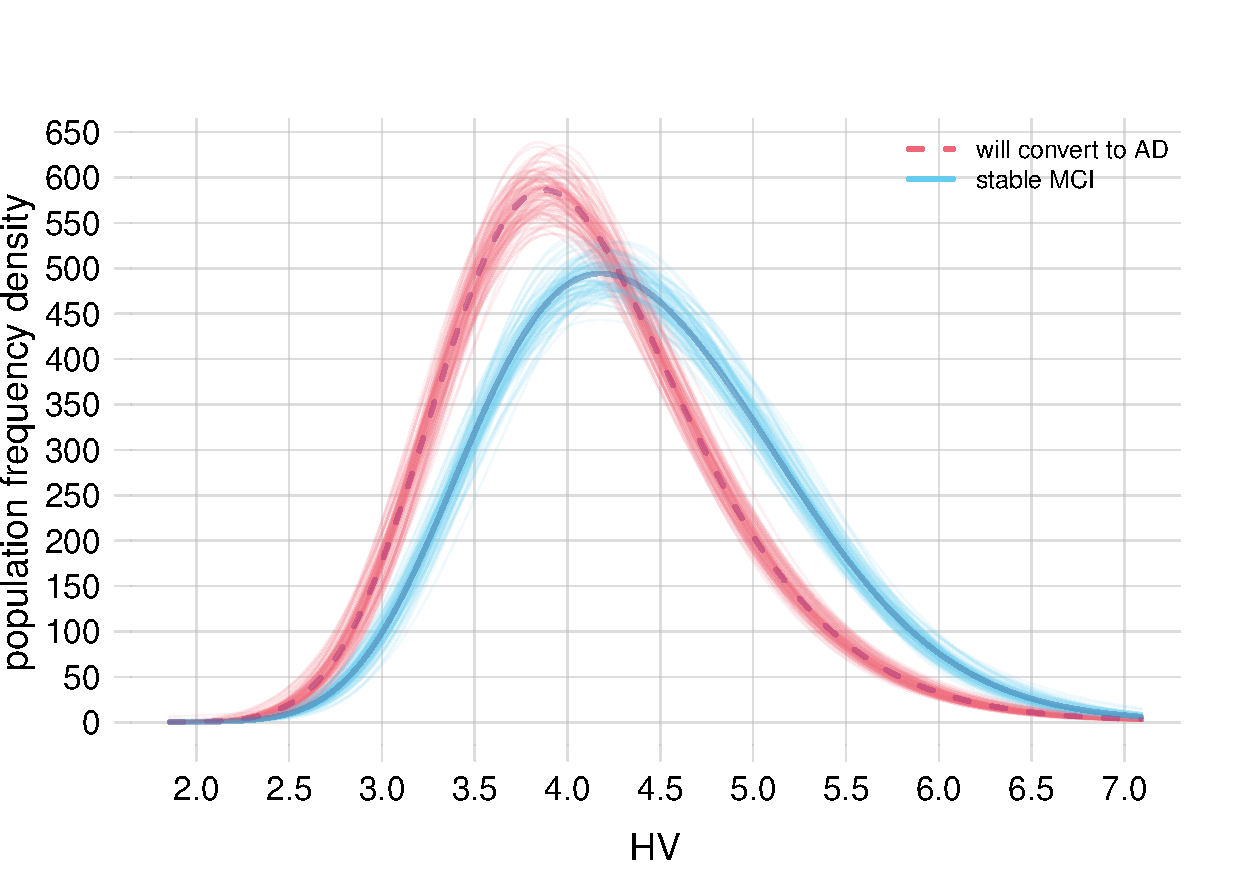
\includegraphics[width=0.43\linewidth]{population_distr_HV.pdf}%
\qquad%
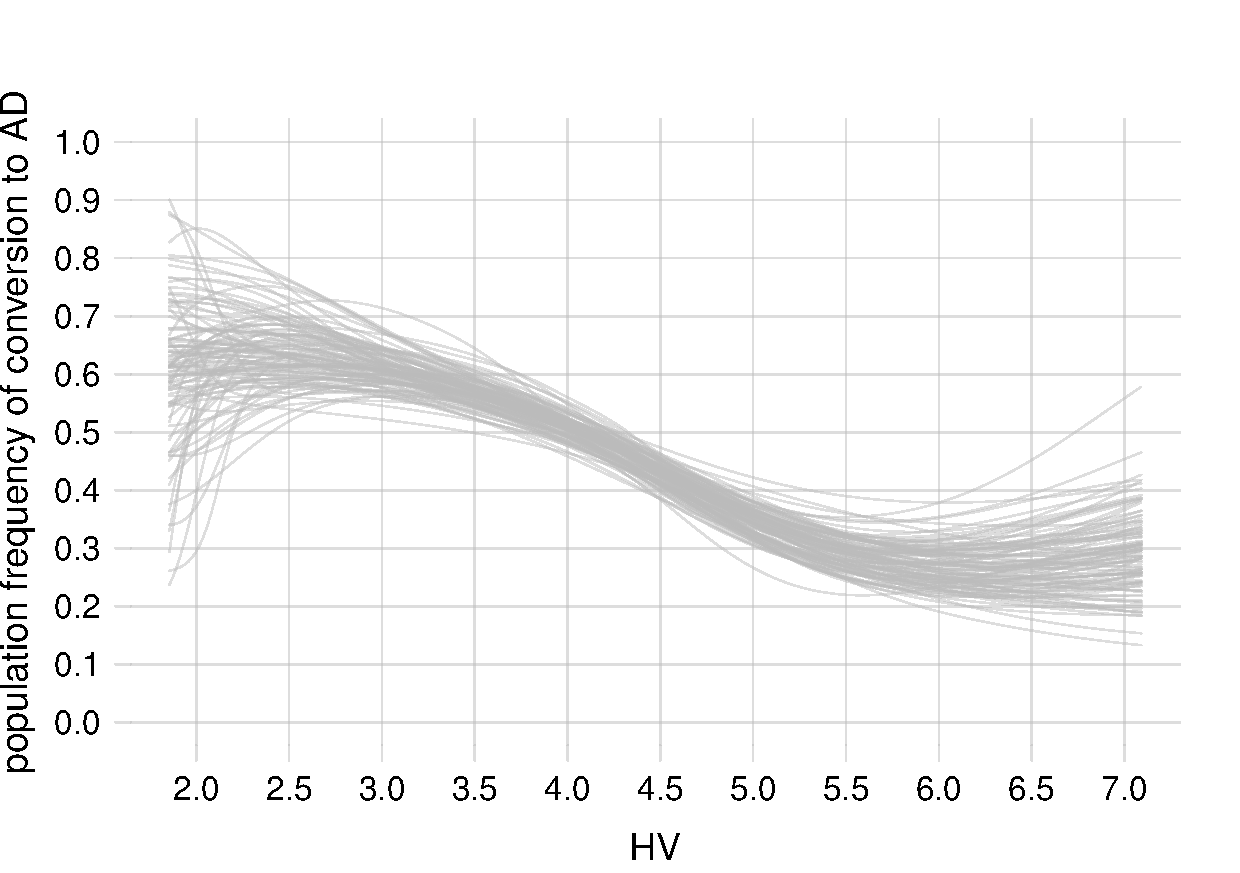
\includegraphics[width=0.43\linewidth]{prob_conversion_HV.pdf}%
\caption{Predicted distributions of some predictor variates, for the subpopulation of patients that will convert to \ad\ (red dashed) and the subpopulation with stable \mci\ (solid blue).}\label{fig:marginal_pop_distributions}
\end{figure}%
%
The two subpopulations of patients are clearly distinct in the \ravltdel, \ravltimm, \hv\ variates. These predictors can yield probabilities of conversion as high as 70\% or as low as 10\%. The two subpopulations are practically indistinguishable in the \gds\ variate, which, therefore, always gives very uncertain predictions.

The learning dataset comprises enough data to greatly reduce our uncertainty about the population distributions, as evident from the very narrow spread of the curves. These simple results show the great usefulness of the \ljm\ for general medical research.


\subsection{Patient's clinical information}
\label{sec:predictor_step}

The 12 predictor values for our four patients are reported in table~\ref{tab:patients_data}, top. Note that Curtis's value for the Hippocampal Volume is missing; this is not a problem for the \ljm. Given these predictor values the \ljm\ can output any probabilities of interest to the clinician. Table~\ref{tab:patients_data}, bottom, reports three probabilities that are important for the step of the next subsection:\footnote{All relative uncertainties of the results are below 0.8\%, Curtis's two likelihoods being an exception at 2\%.}
 % (owing to the illustrative character of this example, we do not fully follow the standards for the expression of measurement uncertainty \citep{jcgm1993_r2008})
\begin{itemize}
\item $\p(\cad\mo\yes \| \predictors)$: the probability that the patient will convert to \ad, given the patient's specific predictors and that the patient comes from the same population as the learning dataset.
\item $\p(\predictors \| \cad\mo\yes)$: the probability that a patient who will convert to \ad\ would have these specific predictor values. In other words, the \emph{likelihood}\footnote{$\p(A\|B)$ is the probability of $A$ given $B$, as well as the likelihood of $B$ given $A$ \citep[\sect~6.1]{good1950}.} of conversion to \ad, given the predictors.
\item $\p(\predictors \| \cad\mo\no)$: the probability that a patient who will remain with stable \mci\ would have these specific predictor values. In other words, the \emph{likelihood} of stable \mci, given the predictors.
\end{itemize}

\begin{table}[!b]
  \centering
  \begin{tabular}[b]{lcccc}
    \hline\\[-1.5\jot]
    &{\small Olivia} &{\small Ariel} &{\small Bianca} &{\small Curtis}
    \\[2\jot]
    \age&75.4&75.4&75.4&63.8 \\
    \sex&F&F&F&M \\
    Hippocampal volume (\hv)${}/10^{-3}$&4.26&4.26&4.26&[missing] \\
    \apoe\ status&\no&\no&\no&\yes \\
    Reading test (\anart)&18&18&18&15 \\
    Category Fluency Test (\cft)&21&21&21&14 \\
    Geriatric Depression Scale (\gds)&3&3&3&2 \\
    \ravltimm\,ediate memory &36&36&36&20 \\
    \ravltdel\,ayed recall &5&5&5&0 \\
   \ravltrec\,ognition &10&10&10&3 \\
    Trail Making Test A (\tmta)&21&21&21&36 \\
    Trail Making Test B (\tmtb)&114&114&114&126
    \\[\jot]
    \hline\\
    {\small $\p(\cad\mo\yes \| \predictors)$}&
    0.302&0.302&0.302&0.703
    \\
    {\small $\p(\predictors \| \cad\mo\yes)/10^{-12}$}&
    8.97&8.97&8.97&1.14
    \\
    {\small $\p(\predictors \| \cad\mo\no)/10^{-12}$}&
    18.6&18.6&18.6&0.343
    \\[\jot]
    \hline
  \end{tabular}\hfill
  \caption{Predictor values for the four patients, and resulting conditional probabilities}\label{tab:patients_data}
\end{table}
% \begin{table}[!b]
%   \centering
%   \begin{tabular}{lcccc}
%     \hline\\[-1.5\jot]
%     &{\small Olivia} &{\small Ariel} &{\small Bianca} &{\small Curtis}
%     \\[\jot]
%     {\small $\p(\cad\mo\yes \| \predictors)$}&
%     0.302&0.302&0.302&0.703
%     \\
%     {\small $\p(\predictors \| \cad\mo\yes)/10^{-12}$}&
%     8.97&8.97&8.97&1.14
%     \\
%     {\small $\p(\predictors \| \cad\mo\no)/10^{-12}$}&
%     18.6&18.6&18.6&0.343
%     \\[\jot]
%     \hline
%   \end{tabular}
%   \caption{\mynotep{Probabilities computed by the \ljm}} \label{tab:prob_likelihoods_patients}
%   \end{table}

The \ljm\ can also answers other questions of interest to the clinician. For instance, what could be the value of Curtis's Hippocampal Volume? The answer is given in \fig~\ref{fig:curtis_HV}, which also shows the full-population distribution as comparison (dashed grey); with 95\% probability Curtis's value is between 2.8 and 5.3, with a median of 3.8. And what is the frequency of conversion to \ad\ among the subpopulation having Olivia's, Ariel's, or Bianca's predictors? The answer is given in the histogram of \fig~\ref{fig:freq_distribution_patients}: with 95\% probability, the fraction of this subpopulation that eventually converts to \ad\ is between 0.19 and 0.43; this uncertainty range is due to the limited size of the learning dataset. The probability $\p(\cad\mo\yes \| \predictors)$ is equal to the average of such a distribution \citep[\eg][\sects~4.2--4.3]{bernardoetal1994_r2000}, provided the patient and dataset can be considered as coming from the same population.

  

\begin{subfigure}[t]\setcounter{subfigure}{0}
  \centering%
  \begin{minipage}[t]{0.49\linewidth}\centering
    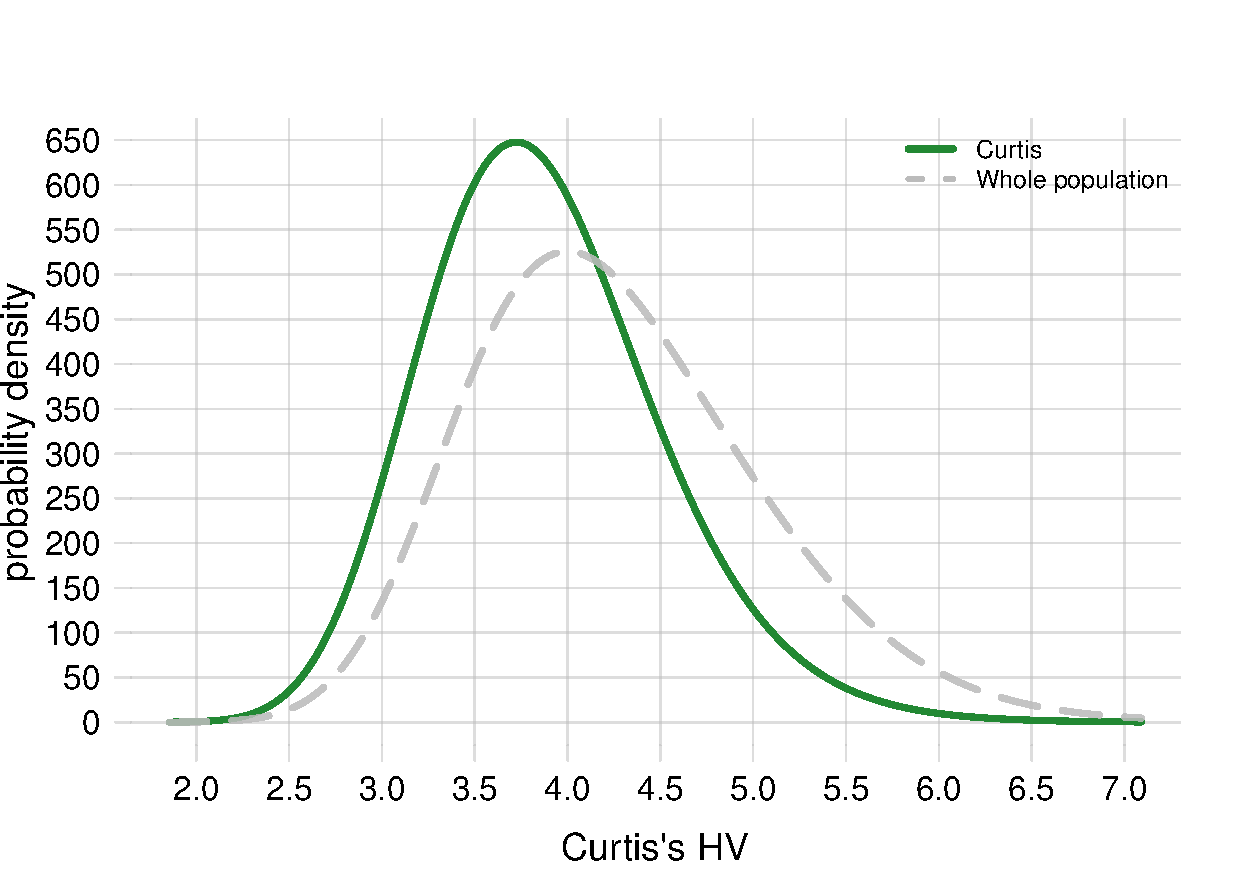
\includegraphics[width=\linewidth]{curtis_distr_HV.pdf}
\caption{Probability distribution for Curtis's Hippocampal Volume}\label{fig:curtis_HV}
  \end{minipage}\hfill%
  \begin{minipage}[t]{0.49\linewidth}\centering
    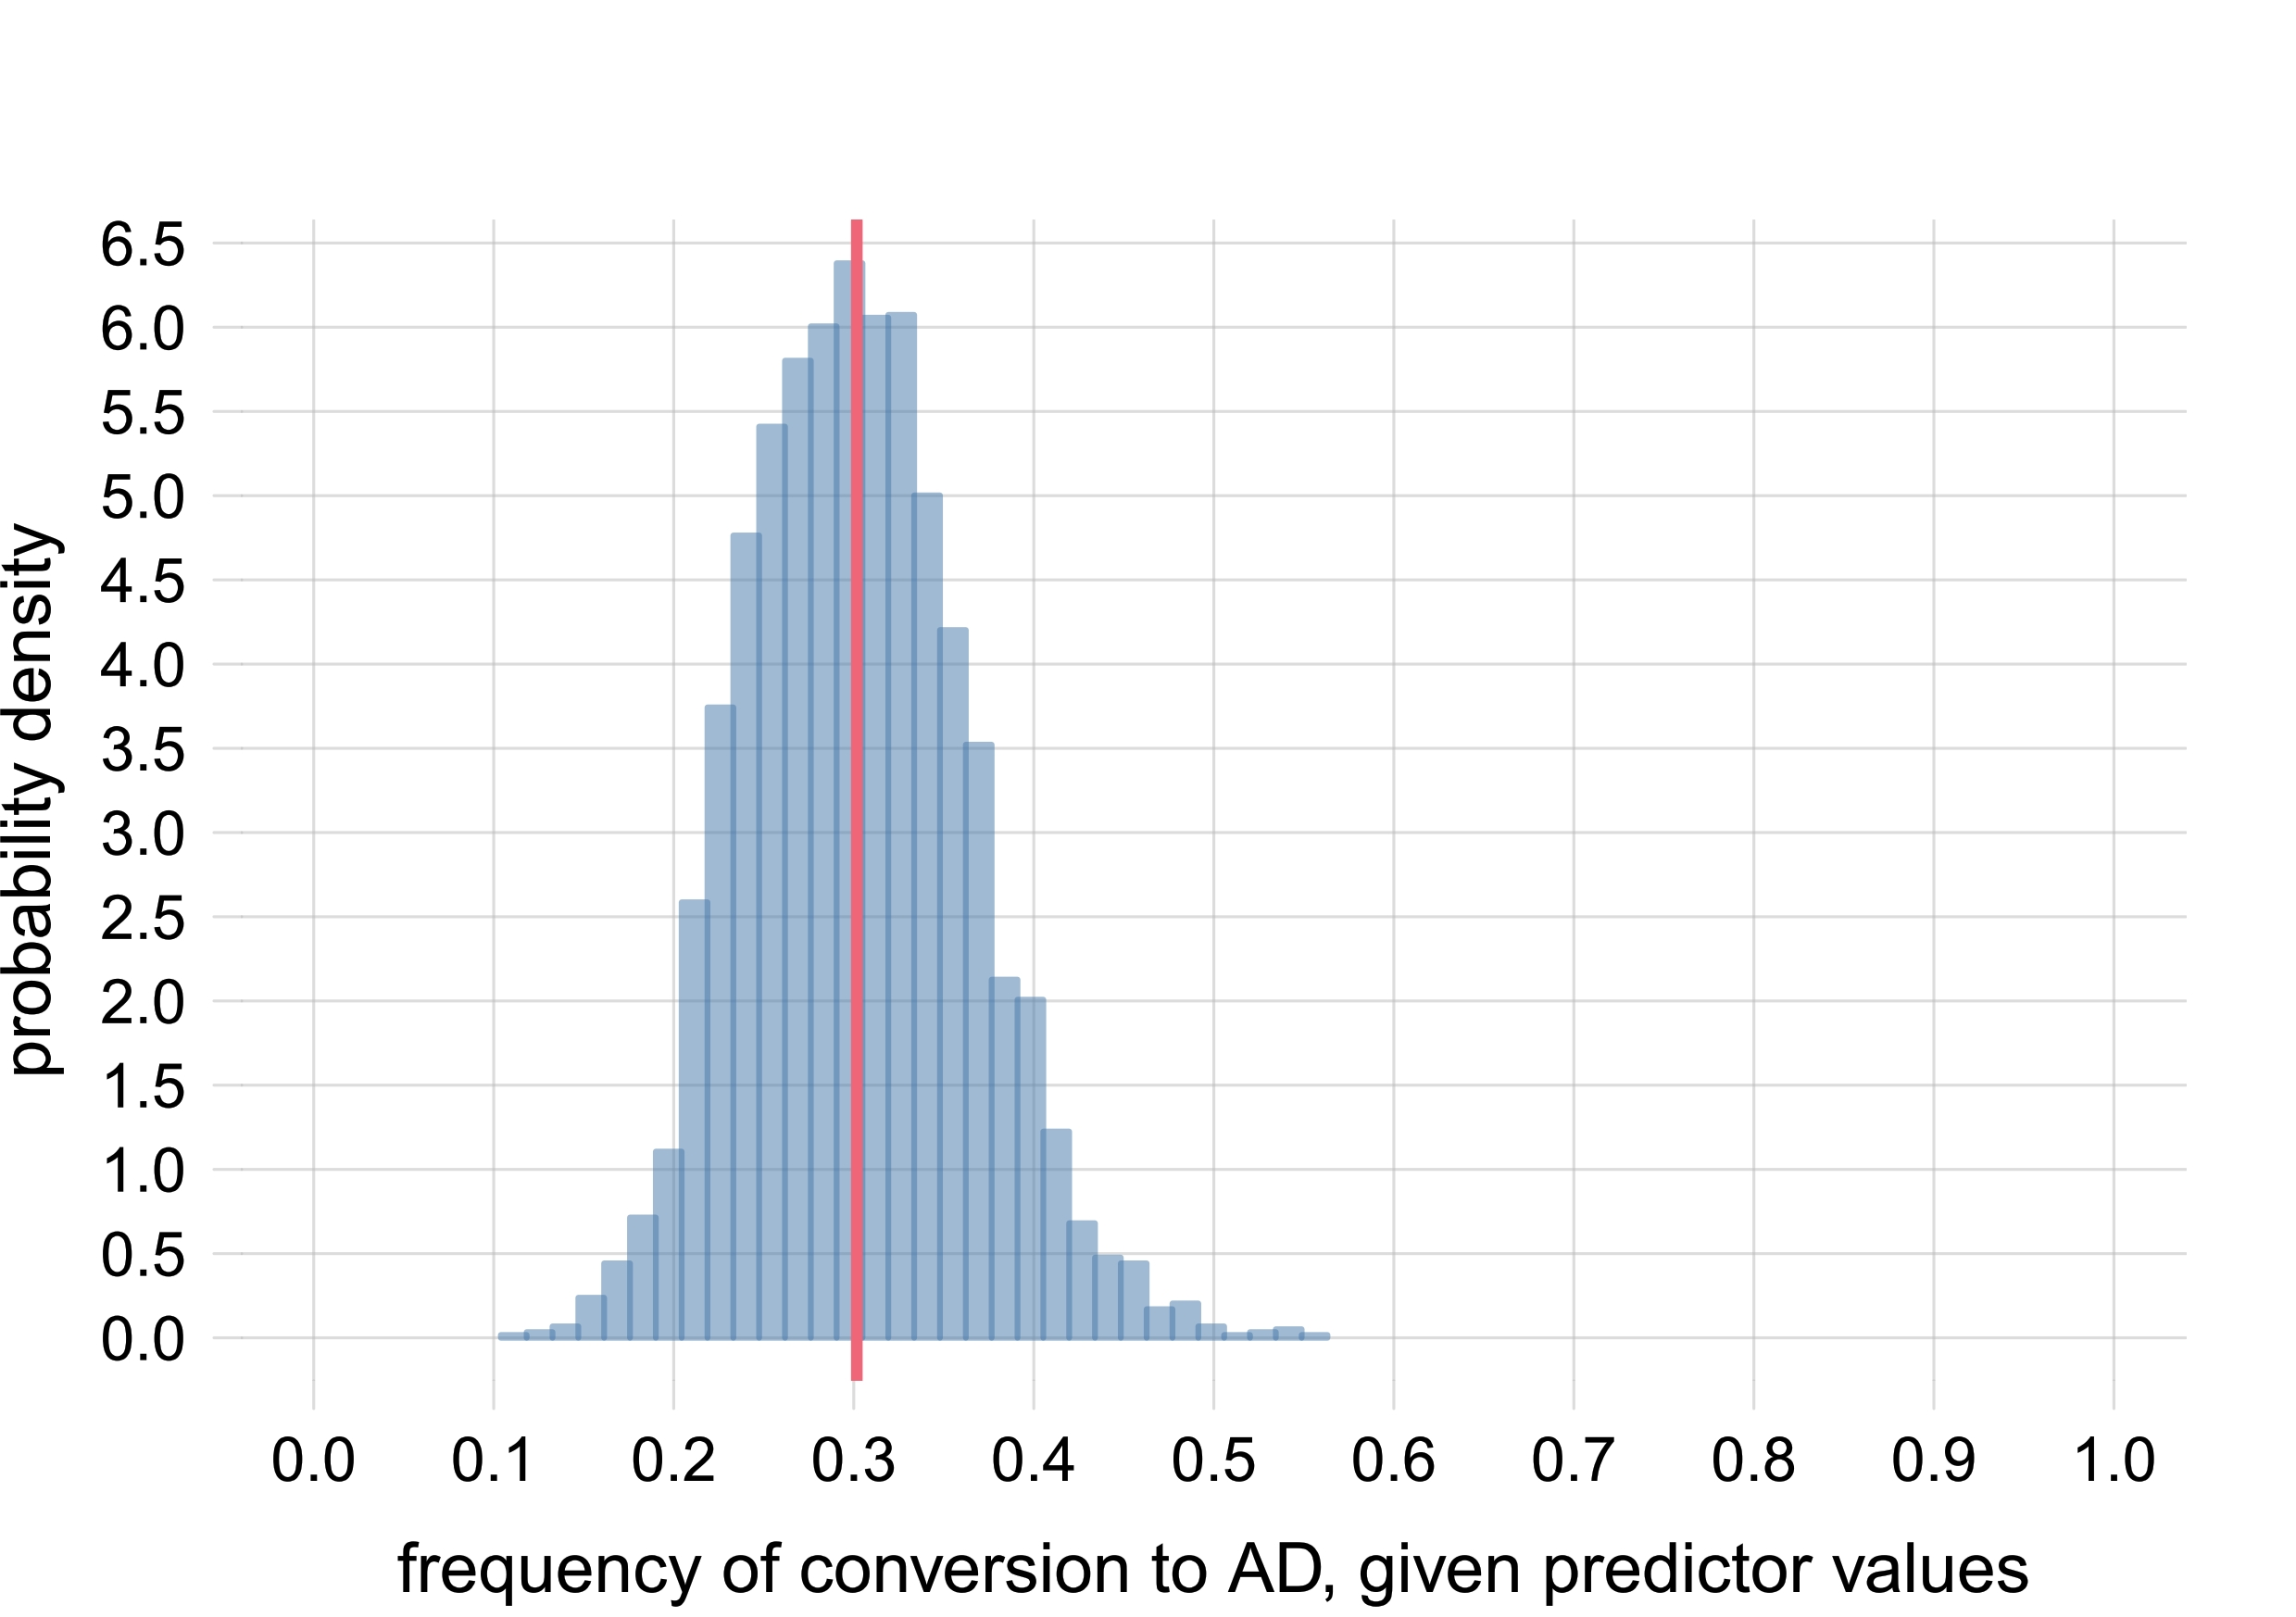
\includegraphics[width=\linewidth]{directprob_olivia.pdf}
%    \\ \footnotesize Olivia, Ariel, Bianca
    \caption{Probability distribution for the frequency of conversion to \AD, among the subpopulation having Olivia's, Ariel's, or Bianca's predictors. The red vertical line is the value of the probability $\p(\cad\mo\yes \| \predictors)$.}\label{fig:freq_distribution_patients}
  \end{minipage}
  % \hfill
  % \begin{minipage}{0.49\linewidth}\centering
  %   \includegraphics[width=\linewidth]{directprob_curtis.pdf}\\
  %   \footnotesize Curtis
  % \end{minipage}
\end{subfigure}%



%%%% MI given all minus ...
%      AVDEL30MIN_neuro RAVLT_immediate TRABSCOR_neuro AVDELTOT_neuro LRHHC_n_long
% mean            0.125           0.131          0.135          0.137        0.138
% sd              0.004           0.004          0.004          0.004        0.004
%      TRAASCOR_neuro CATANIMSC_neuro   AGE GDTOTAL_gds ANARTERR_neuro Gender_num_
% mean          0.139           0.139 0.139       0.140          0.140       0.140
% sd            0.004           0.004 0.004       0.004          0.004       0.004
%      Apoe4_   all
% mean  0.140 0.140
% sd    0.004 0.004


%%%% MI differences: 
%        all    Apoe4_ Gender_num_ ANARTERR_neuro GDTOTAL_gds      AGE CATANIMSC_neuro
% mean 0.000 0.0000121   0.0000939       0.000264    0.000295 0.000512        0.000561
% sd   0.009 0.0090000   0.0090000       0.009000    0.009000 0.009000        0.009000
%      TRAASCOR_neuro LRHHC_n_long AVDELTOT_neuro TRABSCOR_neuro RAVLT_immediate
% mean        0.00113      0.00187        0.00234        0.00438         0.00905
% sd          0.00900      0.00900        0.00900        0.00900         0.00800
%      AVDEL30MIN_neuro
% mean           0.0144
% sd             0.0080






\bigskip% Newpage break just to help while writing the draft
\subsection{Assessment of population and auxiliary information}
\label{sec:population_step}

\subsubsection{Rationale}
\label{sec:population_step_rationale}

As already mentioned, and as will be discussed more in detail in the next section, the clinician needs a probability in order to choose a treatment or other course of action about the current patient. This probability is computed by generalizing associations between predictors and predictand hidden in a dataset of similar patients. The way this generalization is made, however, can differ from patient to patient in two respects:
\begin{itemize}
\item Only some particular, directed associations can be generalized to the current patient, whereas others would be inappropriate to generalize. In some cases, for example when the learning dataset is artificially assembled with balancing or stratification methods, some associations cannot be generalized to any patients at all.
\item There can be additional information available for the current patient, for instance some clinical predictors not included in the learning dataset, or other \enquote{softer} information such as family history or geographic background.
\end{itemize}
There is no sharp separation between these two items. The presence of additional information often automatically implies that some associations cannot be generalized from the learning dataset to the current patient.


\setlength{\intextsep}{0ex}% with wrapfigure
\setlength{\columnsep}{1ex}% with wrapfigure
\begin{wrapfigure}{r}{0.25\linewidth}% with wrapfigure
%\vspace{-1ex}%
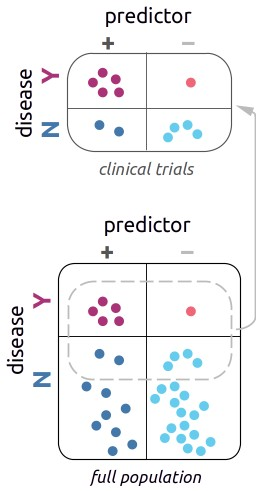
\includegraphics[width=\linewidth]{baseratefallacy3.png}%
% \includegraphics[width=\linewidth]{baseratetrials.png}\\[\jot]
% \includegraphics[width=\linewidth]{baseratepopulation.png}
\end{wrapfigure}%
Let us explain with a familiar example why particular associations cannot be generalized. Most medicine students learn about the \emph{base-rate fallacy} \citep{barhillel1980,jennyetal2018,sprengeretal2021,matthews1996}. Consider a large set of clinical trials, illustrated in the upper table on the side, where each dot represents, say, 10\,000 patients. In this sample dataset it is found that, among patients having a particular value \enquote{+} of some predictors (left column), 71.4\% (or 5/7, upper square) of them eventually developed a disease. The fallacy lies in judging that a new real patient from the full population, who has that particular predictor value, also has a 71.4\% probability of developing that disease. In fact, \emph{this probability will in general be different}. In our example it is 33.3\% (5/15), as can be seen in the lower table illustrating the full population. This difference would be noticed as soon as the inappropriate probability were used to make prognoses in the full population.

There is a discrepancy in the conditional frequencies of predictand given predictors, between the sample dataset and the full population, because the proportion of positive vs negative disease cases in the latter has some value, 16.7\%/83.3\% in our example, whereas the samples for the trials (dashed line in the lower table) were chosen so as to have a 50\%/50\% proportion. This sampling procedure is called \enquote{class balancing} in machine learning \citep{provost2000,drummondetal2005,weissetal2003}. More generally this discrepancy can appear whenever a population and a sample dataset from it do not have the same frequency distribution for the predictand. In this case we cannot rely on the probabilities of \enquote{predictand given predictors} obtained from the sample dataset, which we symbolically write as
\begin{equation}
  \p(\predictand \| \predictors, \dataset)
\end{equation}
\mynotew{Maybe make clear at the beginning that we denote predictand with $Y$, predictors with $X$, dataset with $D$, and just write $\p(Y\|X\,D)$?}

A little counting in the side figure reveals, however, that other frequencies may be relied upon. Consider the full population. Among all patients who developed the disease, 83.3\% (or 5/6, upper row) of them had the particular predictor value, while among those who did not develop the disease, 33.3\% (or 1/3, lower row) had the particular predictor value. \emph{And these frequencies are the same in the sample dataset}. These frequencies from the clinical trials can therefore be used to make a prognosis using Bayes's theorem:
\begin{equation}
  \label{eq:base-rate_correction}
  % \p(\predictand \| \predictors) \propto
  % \p(\predictors \| \predictand,
  % \dataset)
  % \cdot   \p(\predictand \| \texttt{\small population})
  \p(\predictand \| \predictors) =
  \frac{
    \p(\predictors \| \predictand,
  \dataset)
  \cdot   \p(\predictand \| \population)
}{\sum\limits_{\predictand}
    \p(\predictors \| \predictand,
  \dataset)
  \cdot   \p(\predictand \| \population)
}
\end{equation}
In our example we find
\begin{equation}
  \label{eq:base-rate_correction_example}
 \begin{split}
  % \p(\predictand \| \predictors) \propto
  % \p(\predictors \| \predictand,
  % \dataset)
  % \cdot   \p(\predictand \| \texttt{\small population})
   \p(\diseasep \| \predictorp)
   &=
  \frac{
    \p(\predictorp \| \diseasep,
  \trials)
  \cdot   \p(\diseasep \| \population)
}{
  \biggl[\begin{aligned}
    &\p(\predictorp \| \diseasep,
  \trials) 
  \cdot   \p(\diseasep \| \population)
  +{}\\[-0.5\jot]&\hspace{5em}
    \p(\predictorp \| \diseasem,
  \trials)
  \cdot   \p(\diseasem \| \population)
\end{aligned}\biggr]
} \\[2\jot]
&\approx
  \frac{ 0.833 \cdot 0.167}{0.833 \cdot 0.167 + 0.333 \cdot 0.833}
  = 0.33
  \end{split}
\end{equation}
which is indeed the correct full-population frequency.

If the samples of the clinical trials had been chosen with the same frequencies as the full population (no \enquote{class balancing}), then the probability $\p(\predictand \| \predictors, \dataset)$ from the dataset would be the appropriate one to use. But the probabilities $\p(\predictors \| \predictand, \dataset)$ together with Bayes's theorem as in \eqn~\eqref{eq:base-rate_correction} would also lead to exactly the same probability. We thus see that \emph{using the probabilities}
\[\p(\predictors \| \predictand, \dataset)\]
\emph{from the dataset is preferable to using} $\p(\predictand \| \predictors, \dataset)$. The former yield the same results as the latter when use of the latter is appropriate, and allow us to apply corrections when use of latter is inappropriate. The superiority of using $\p(\predictors \| \predictand, \dataset)$ probabilities is illustrated with a toy example in table~\ref{tab:superiority_predictors_given_predictand}.
\begin{table}[t]
  \begin{framed}
  \small
  \caption{\small\bf superiority of the \enquote{predictors$\pmb{\|}$predictand} approach}
  \label{tab:superiority_predictors_given_predictand}
  \mbox{}\\
  We split our learning dataset in two subsets:
    \begin{itemize}
    \item One with 361 datapoints and a ratio of 29.9\%/70.1\% of conversions to \ad\ vs stable \mci. This is used as learning set.
    \item One with 343 datapoints and a ratio of 63.3\%/36.7\% of conversions to \ad\ vs stable \mci. This is used as a fictive full population.
    \end{itemize}
    This partition was made with no systematic sampling of any variates except the conversion variate.

    We then make a prognosis for each of the 343 \enquote{new} patients, through four separate approaches: (a) using the probabilities $\p(\predictand \| \predictors, \dataset)$, as typical of machine-learning algorithms; (b) using $\p(\predictors \| \predictand, \dataset)$ together with the base rate, as explained above; (c) tossing a coin; (d) always prognosing \enquote{conversion to \ad}, which guarantees 63.3\% correct prognoses owing to the base rate. The accuracies (number of prognoses giving more than 50\% probability to the correct course) of these four approaches are finally calculate. Here are the results from lowest to highest:

    \medskip
    { 
      % \begin{table}[!h]
      \centering
      \begin{tabular}{cccc}
        \hline\\[-\jot]
        {\scriptsize predictand$\|$predictors}&{\scriptsize coin toss}&{\scriptsize always predict conversion}&{\scriptsize predictors$\|$predictand \amp\ base\,rate}
        \\[1\jot]
        37.3\% & 50\% & 63.3\% & 73.2\%\\[\jot]
        \hline
      \end{tabular}
      % \end{table}

    }
    \medskip
    
    The \enquote{predictand$\|$predictors} approach leads to worse results than a coin toss because of its underlying base-rate fallacy. The \enquote{predictors$\|$predictand} approach leads to better results than simply always prognosing the most common base-rate outcome; this shows that the dataset can still provide useful statistical information despite its mismatched base rate. Inference algorithms that only yield \enquote{predictand$\|$predictors} outputs, unlike the \ljm, are incapable of extracting this useful information.
  \end{framed}
\end{table}

\medskip

The use of dataset probabilities different from $\p(\predictand \| \predictors, \dataset)$ can be necessary even when the dataset has statistics identical with the population it is sampled from. Typical cases are the prognosis of a patient that comes from a peculiar subpopulation or even from a different population \citetext{\citealt{lindleyetal1981}; \citealt{quintanaetal2017}; \citealt[\chap~4]{soxetal1988_r2013}; \citealt[\chap~5]{huninketal2001_r2014}}. The first case happens for instance when the clinician has additional information not included among the predictor variates, such as the result of an additional clinical test, or family history. The second case happens for instance when the patient comes from a different geographical region. There is of course no sharp distinction between these two cases.

What is important is that in either case it can still be possible to use statistical information from the sample dataset to make prognoses. It is sufficient that some \emph{conditional} statistics may be applicable to the specific patient. For a patient coming from a different region, for example, it may be judged that the conditional probabilities $\p(\predictand \| \predictors, \dataset)$ still apply. In other words, the patient may still be considered of a member of the subpopulation having those specific predictor values. Using more technical language we say that a new patient can be considered \emph{exchangeable} with the patients constituting the dataset, but only conditional on particular variates. See Lindley \citetext{\citeyear[especially around \sects~7.3, 8.6]{lindley2006_r2014}; \citeyear{lindleyetal1981}} for a clear and logically impeccable presentation not obscured by technical language \citetext{more technical references are \citealt[\sects~4.2--4.3]{definetti1930,definetti1937,dawid2013,bernardoetal1994_r2000}; see also \citealt{malinasetal2004_r2016}, \citealt{sprengeretal2021} about confounding and Simpson's paradox, to which this topic is tightly related}.

This topic is complex and of extreme importance for inference, but its detailed study is not the goal of the present work. Our main point here is that population variability and auxiliary clinical information are important factors that differentiate patients, and a personalized approach ought to take them into account. The method here presented does this naturally, allowing a great flexibility in selecting which statistical features of the sample dataset should be used for each new patient, and the integration of auxiliary clinical information in the form of a prior probability. As discussed in \sect~\ref{sec:predictor_step}, the \ljm\ allows us to quickly calculate conditional probabilities $\p(Y\|X, \dataset)$ for any desired variate subsets $Y$ and $X$ required by the patient's relevant population.




\subsubsection{Application to the example study}
\label{sec:posterior_application}

In our example of \sect~\ref{sec:four_patients}, all statistics of the dataset are considered relevant for Olivia, Bianca, and Curtis. For these patients the clinician can therefore use Bayes's theorem with the likelihoods of table~\ref{tab:patients_data} and the dataset conversion rate of $0.463$ -- or equivalently directly the probabilities $\p(\cad\mo\yes \| \predictors, \dataset)$ provided in the same table.

For Ariel, however, the clinician judges that a different base rate or prior probability of conversion should be used, equal to 65\%, because of her different geographical origin and family history. In her case the clinician uses Bayes's theorem with the likelihoods of table~\ref{tab:patients_data} and the prior probability of $0.65$.

The final probabilities of conversion to \ad\ for our four patients are reported in table~\ref{tab:posterior_patients}. Note how the final probability for Ariel is higher than that for Olivia and Bianca, even if the predictor data are the same for these three patients.

\medskip
\begin{table}[!h]
  \centering
  \begin{tabular}{lcccc}
    \hline\\[-1.5\jot]
    &{\small Olivia} &{\small Ariel} &{\small Bianca} &{\small Curtis}
    \\[\jot]
    {\small initial probability\; $\p(\cad\mo\yes \| \texttt{\footnotesize auxiliary\,info})$}&
    0.463&0.65&0.463&0.463
    \\[\jot]
    {\small final probability\; $\p(\cad\mo\yes \| \predictors, \dataset, \texttt{\footnotesize auxiliary\,info})$}&
    0.302&0.47&0.302&0.703
    \\[\jot]
    \hline
  \end{tabular}
    \caption{Final probabilities of conversion computed from dataset and auxiliary information}\label{tab:posterior_patients}
\end{table}


\bigskip% Newpage break just to help while writing the draft
\subsection{Assessments of treatments and benefits; final decision}
\label{sec:utilities_step}

\subsubsection{Rationale}
\label{sec:expected_utility_theory}


A crucial point in clinical decision-making is this: the clinician needs to assess, not the presence (present or future) of a disease, but the \emph{risk} of its presence. Is there a difference between these two problems? and why is the difference important?

In clinical practice we can rarely diagnose or prognose a medical condition with full certainty. Perfect classification is therefore impossible. But also a \enquote{most probable} classification, which may be enough in other contexts, is inadequate in clinical ones. The problem is that the clinician has to decide among different courses of actions, such as different treatments, more tests, and so on, and the optimal one depends on \emph{how probable} the medical condition is, not just on whether it is more probable than not.

Two examples illustrate this point. Say there is a dangerous treatment that extends the patient's lifetime by one year if the disease is actually on its course, but shortens the patient's lifetime by five years if the disease is actually not present. Obviously the clinician cannot prescribe the treatment just because the disease is \enquote{more probably present than not}. If 60 out of 100 treated similar patients actually develop the disease (so \enquote{more probable than not} is correct), the clinician has added $1 \times 60 = 60$ years \emph{but subtracted $\mathit{5 \times 40 = 240}$ years} from their combined lifespans. As an opposite example, say a less dangerous treatment extends the patient's lifespan by five years if the disease is on its course, but shortens it by one month if the disease is not present. In this case it may be advisable to undergo the treatment even if the disease is \emph{less} probably present than not. If 20 out of 100 treated similar patients develop the disease, the clinician has added $5 \times 20=100$ and subtracted $\tfrac{1}{12} \times 60=5$ years to their combined lifespans.

In both examples it is clearly important to assess the \emph{probability} that the patient will develop the disease. And the \ljm, as explained in the previous sections, gives us such probabilities.

But the choice between treatments does not only rely on the probability of the medical condition. Here is where differences between patients vary and matter the most. Consider again the second example above, about the less dangerous treatment. Let us add that the treatment would extend the lifespan by five years, but would also somewhat worsen the quality of life of the patient and the patient's family. Suppose our patient is quite old and tired, has had a happy life, and is now looking with a peaceful mind towards death as a natural part of life. Such a patient may prefer to forego the bother of the treatment and the additional five years even if the probability for the disease is quite high.

The benefits of the different treatments, and the probability thresholds at which one treatment becomes preferable to another, must therefore be judged and quantified primarily by the patient. Utility theory and maximization of expected utility allow clinician and patient to make such judgements and decisions in a coherent way \citetext{\citealt{soxetal1988_r2013,huninketal2001_r2014}; see also the clear and charming exposition by \citealt{lindley1971_r1988}, and \citealt{ohaganetal2006}}.

We summarize the main, patient-dependent procedure for decision making, and show how our computations so far fit perfectly with it.

The clinician first assesses and list the mutually exclusive courses of actions available for the specific patient. These could be treatments, more tests, do nothing, and so on. Often there are \emph{sequences} of decision available, but the utility framework can be applied to them as well \citep[see references above and][]{raiffa1968_r1970}. The list of courses of action is already patient-dependent: some alternatives may not be suitable (say, owing to allergies), some may be economically too costly, and so on.

Each course of action will have different consequences, which additionally depend on the patient's unknown clinical condition of interest. A treatment may have some consequences if the patient has or will develop the disease, and different consequences otherwise. The patient quantifies, with the clinician's guidance, the benefits and costs -- technically called \enquote{utilities} -- of such possible consequences. The quantification of utilities is not within the scope of the present work. The references cited above offer several guidelines and rules for numerically translating factors such as quality of life and expected lifespan into utilities.

The courses of actions, uncertain clinical conditions, and the quantified utilities $U$ of their consequences can be organized into a table of this form:
  \begin{center}
    \begin{tabular}{cccc}
      &{\small clinical condition $a$}&{\small clinical condition $b$}&{\small \ldots}
      \\[2\jot]
      {\small action $\alpha$} & $U_{\alpha a}$ & $U_{\alpha b}$ &$\dotso$ \\[\jot]
      {\small action $\beta$} & $U_{\beta a}$ & $U_{\beta b}$ &$\dotso$ \\[\jot]
      {\small \ldots} &$\dotso$&$\dotso$&$\dotso$
    \end{tabular}
  \end{center}
which can be compactly represented by a so-called \emph{utility matrix} $\bigl(U_{ij})$, the row index $i$ enumerating the actions, and the column index $j$ the clinical conditions. Note that the number of possible treatments and of clinical conditions do not need to be equal; generally they are not.

The \emph{expected utility} $\eU_{i}$ of an action $i$ is calculated as the expectation of its utilities $U_{ia}, U_{ib}, \dotsc$ with respect to the probabilities $\p(a), \p(b), \dotsc$ of the clinical conditions $a,b,\dotsc$:
\begin{equation}
  \label{eq:def_expected_utility}
  \eU_{i} \defd U_{ia}\, \p(a) + U_{ib}\, \p(b) + \dotsb
\end{equation}
Note that this corresponds to a matrix multiplication between the matrix of utilities and the vector of probabilities.

Finally, the recommended action is the one having \emph{maximal expected utility}.

\mynotep{Add a couple of comments about the inevitability of the rules of decision theory \citep{lindley1971_r1988}}



\subsubsection{Application to the example study}
\label{sec:expected_utility_application}

At present there are no cure for \ad, although some recent pharmacological agents are shown to extend the time before a patient is cognitively severely impaired \mynotew{ref}. But for the sake of our case study let us imagine that there, in the near future, are three mutually exclusive treatment options for prevention or retardation of the disease; call them $\beta$, $\gamma$, $\delta$. And denote the simple option of \enquote{no treatment} by $\alpha$. The clinical conditions to be considered are just two: the patient will have stable \mci, or will convert to \ad. Denote them by $\nAD$ and $\AD$.

We have therefore $4 \times 2 = 8$ possible consequences of the four treatments depending on the two clinical conditions. Our four patients and clinician quantify the utilities, arriving at the utility matrices shown in table~\ref{tab:utilities_patients}. Note that Olivia, Ariel, Curtis quantify the benefits of the treatments in exactly the same way, but Bianca's quantification differs slightly \mynotew{add an example of why}.

\medskip
\begin{table}[!h]
  \centering
  \begin{tabular}{lccccccc}
    \hline\\[-1.5\jot]
    &{\small Olivia} &&{\small Ariel} &&{\small Bianca} &&{\small Curtis}
    \\[\jot]
    $\begin{matrix}&\\
      \text{treatment }\alpha\\ 
      \text{treatment }\beta\\ 
      \text{treatment }\gamma\\ 
      \text{treatment }\delta
    \end{matrix}$
    &
    $
    \begin{gathered}
      \begin{smallmatrix}
        \nAD&\AD
      \end{smallmatrix}\\[-\jot]
\begin{bmatrix}10&0\\9&3\\8&5\\0&10\end{bmatrix}
\end{gathered}
$
    &&
    $\begin{gathered}
      \begin{smallmatrix}
        \nAD&\AD
      \end{smallmatrix}\\[-\jot]
      \begin{bmatrix}10&0\\9&3\\8&5\\0&10\end{bmatrix}\end{gathered}$
    &&
    $\begin{gathered}
      \begin{smallmatrix}
        \nAD&\AD
      \end{smallmatrix}\\[-\jot]
      \begin{bmatrix}10&0\\8&3\\7&5\\0&10\end{bmatrix}\end{gathered}$
    &&
    $\begin{gathered}
      \begin{smallmatrix}
        \nAD&\AD
      \end{smallmatrix}\\[-\jot]
      \begin{bmatrix}10&0\\9&3\\8&5\\0&10\end{bmatrix}\end{gathered}$
    \\[6\jot]
    \hline
  \end{tabular}
  \caption{Utility matrices for the four patients}\label{tab:utilities_patients}
\end{table}

The probabilities for the two medical conditions are those found in the previous section, reported in table~\ref{tab:posterior_patients}. For brevity we denote just by $\p(\AD)$ the probability of conversion given a patient's predictor values, and by $\p(\nAD)\equiv 1- \p(\AD)$ the complementary probability of stable \mci, given the same predictor values. The expected utilities of each treatment for each patient can then be easily computed. For example, for Olivia the expected utility of treatment $\beta$ is
\begin{equation}
  \label{eq:utility_olivia_example}
  \eU_{\beta} = 9 \cdot (1-0.463) + 3 \cdot 0.463 = 7.19
\end{equation}
The results for all patients are reported in table~\ref{tab:exp_utilities_patients}, with the maximal expected utilities in \textbf{boldface}.

\medskip
\begin{table}[!h]
  \centering
  \begin{tabular}{lcccc}
    \hline\\[-1.5\jot]
    &{\small Olivia} &{\small Ariel} &{\small Bianca} &{\small Curtis}
    \\[\jot]
    $\begin{matrix}
      \text{treatment }\alpha\\ 
      \text{treatment }\beta\\ 
      \text{treatment }\gamma\\ 
      \text{treatment }\delta\\[\jot]
      \text{optimal}
    \end{matrix}$
    &
    $\begin{matrix}6.98\\\bm{7.19}\\7.09\\3.02\\[\jot]\beta\end{matrix}$
    &
    $\begin{matrix}5.27\\6.16\\\bm{6.58}\\4.73\\[\jot]\gamma\end{matrix}$
    &
    $\begin{matrix}\bm{6.98}\\6.49\\6.40\\3.02\\[\jot]\alpha\end{matrix}$
    &
    $\begin{matrix}2.97\\4.78\\5.89\\\bm{7.03}\\[\jot]\delta\end{matrix}$
    \\[5\jot]
    \hline
  \end{tabular}
  \caption{Expected utilities and optimal treatment for our four patients}\label{tab:exp_utilities_patients}
\end{table}

% ##     olivia    ariel   curtis
% ## 1 0.698321 0.527060 0.297440
% ## 2 0.718993 0.616236 0.478464
% ## 3 0.709496 0.658118 0.589232
% ## 4 0.301679 0.472940 0.702560

% ##     bianca
% ## 1 0.698321
% ## 2 0.649161
% ## 3 0.639664
% ## 4 0.301679

 
% \subsection{Maximization of expected benefit}
% \label{sec:expected_utility_step}

%% Mutual-info results
% MI: 
%                               mean     sd
% GDTOTAL_gds               0.00052096 0.0003
% Gender_num_               0.00320230 0.0008
% Apoe4_                    0.00349680 0.0010
% AGE                       0.00616330 0.0010
% ANARTERR_neuro            0.00686160 0.0010
% TRAASCOR_neuro            0.01329100 0.0020
% TRABSCOR_neuro            0.02385100 0.0020
% CATANIMSC_neuro           0.02425800 0.0020
% LRHHC_n_long              0.02813100 0.0020
% noncog+demog              0.03598000 0.0030
% AVDELTOT_neuro            0.06025100 0.0030
% RAVLT_immediate           0.09243000 0.0040
% AVDEL30MIN_neuro          0.09397900 0.0040
% allminus_AVDEL30MIN_neuro 0.12548000 0.0040
% allminus_RAVLT_immediate  0.13083000 0.0040
% allminus_TRABSCOR_neuro   0.13546000 0.0040
% allminus_AVDELTOT_neuro   0.13761000 0.0040
% allminus_LRHHC_n_long     0.13797000 0.0040
% cog+demo                  0.13798000 0.0040
% allminus_TRAASCOR_neuro   0.13870000 0.0040
% allminus_CATANIMSC_neuro  0.13928000 0.0040
% allminus_AGE              0.13933000 0.0040
% allminus_GDTOTAL_gds      0.13956000 0.0040
% allminus_ANARTERR_neuro   0.13957000 0.0040
% allminus_Gender_num_      0.13974000 0.0040
% allminus_Apoe4_           0.13983000 0.0040
% all                       0.13984000 0.0040



\bigskip% Newpage break just to help while writing the draft
\subsection{Additional information provided by the \ljm}
\label{sec:additional_results}

As already said, the output of the \ljm\ is about the full population of future patients, with all its statistics. This output can therefore be used for additional purposes such as resource planning, imputation of missing data, sensitivity checks, and the investigation of the predictors' importance in the prognosis.

\subsubsection{Resource planning}
\label{sec:resource_planning}

Let us ask the following question: if the learning dataset were representative of the full population, then how often in the long run would a clinician prognose a conversion to \ad\ with probability between 0\%--2\%, or 2\%--4\%, and so on with 50 bins up to 98\%--100\%?

The \ljm\ can answer this question probabilistically; the answer is plotted in \fig~\ref{fig:progn_probs}. Note that the calculation assumes that the \ljm\ will not be regularly updated with new patients' data (the calculation could also be made with the opposite assumption). The light-blue bands are 95\% uncertainty coverage intervals \footnote{for terminology see \citet[C.2.30]{jcgm1993_r2008}. A $p$\% coverage interval or credible interval is an interval containing the true value with $p$\% probability. Note that it is different from a \enquote{confidence interval}, which cannot be interpreted in such a simple way \citetext{\citealp[pp.~165--166]{pratt1961}; \citealp{jaynes1976}; \citealp[\sect~37.3]{mackay1995_r2005}}}; this uncertainty comes from the fact that we are not certain about the full-population frequencies. We see that it is very improbable that many patients will be prognosed with probabilities around 30\%, smaller than 5\%, or larger than 75\%. The full population is likely to be grouped into four or five \enquote{conversion-probability clusters}, as evident from the peaks. %Note that there are correlations, which cannot be shown in this kind of plot, between the fractions at different bins.
\begin{figure}[h]% with figure
  \centering%
%  \includegraphics[width=0.5\linewidth]{distribution_prognostic_probs.pdf}%
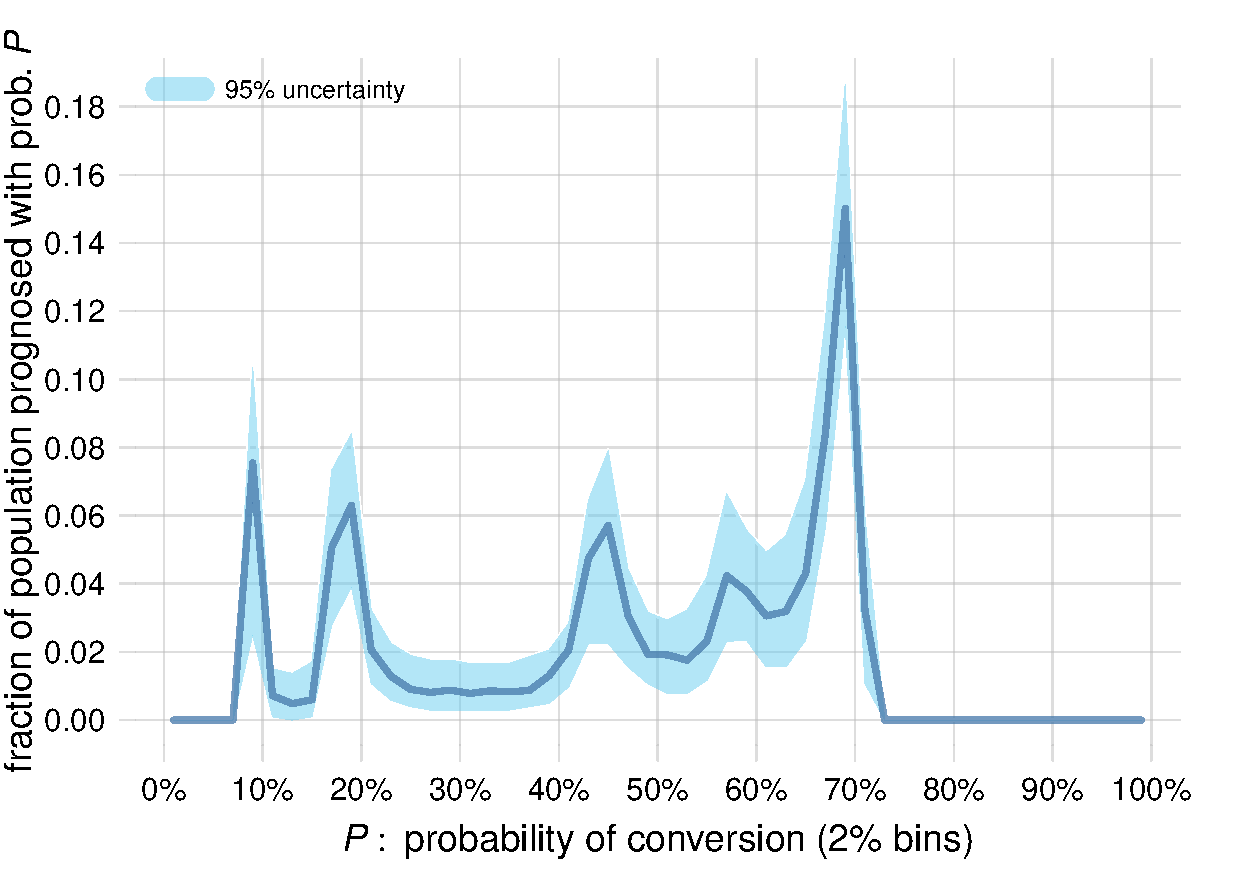
\includegraphics[width=0.75\linewidth]{plotnextpatientconvprob.pdf}%
  \caption{Possible distribution of prognostic probabilities of conversion in the full patient population}\label{fig:progn_probs}
\end{figure}%

This kind of information allows us to make other forecasts of various kinds. For instance, it would be useful to forecast in which proportions the treatments $\alpha,\beta,\gamma,\delta$ (see \sect~\ref{sec:utilities_step}) will be prescribed, assuming that the full population has on average the utility matrix of Olivia, table~\ref{tab:utilities_patients}. We find these coverage intervals with a 90\% probability that the true future proportion will be within each:
\begin{equation}
  \label{eq:ranges_future_treatments}
  \alpha\text{: 21\%--28\%}\qquad
  \beta\text{: 2\%--6\%}\qquad
  \gamma\text{: 31\%--42\%}\qquad
  \delta\text{: 31\%--40\%}
\end{equation}
Again, despite the obvious uncertainties, we can be quite sure that treatments $\gamma$, $\delta$ will be prescribed more often than $\alpha$, and that $\beta$ will be only prescribed in 5\% of cases. This kind of semi-quantitative forecast can be very useful for resource planning.

\subsubsection{Imputation of missing data}
\label{sec:missing_data}

As mentioned in \sect~\ref{sec:predictor_step}, the \ljm\ treats all variates of the learning dataset on the same footing. This is why it can output probabilities \enquote{predictand$\|$predictors}, \enquote{predictors$\|$predictand}, and other combinations with equal ease, exploiting them to correct subpopulation mismatches as illustrated in \sect~\ref{sec:population_step}.

This feature allows us to impute missing data for one or more patients, giving a probability distribution of what those data could be. Such imputation can be done at prognostic time, for sensitivity checks; we discuss this more in detail in the next section. The imputation can also be done a posteriori, possibly years later, when the actual predictand value becomes known. This can be useful for many purposes, for instance the comparison of biological hypotheses.


\subsubsection{Sensitivity checks}
\label{sec:sensitivity}

The imputation of missing data at prognostic time is useful for various kinds of sensitivity analysis.

Let us consider for instance the case of Curtis, whose value of Hippocampal Volume is missing (table~\ref{tab:patients_data}). His clinician thus wonders if the acquisition of this value could lead to a different treatment. The \ljm\ can give a probabilistic answer to this question.

The clinician uses the \ljm\ to find the probability distribution of Curtis's expected utilities (see table~\ref{tab:exp_utilities_patients}) \emph{if the Hippocampal Volume had been known}. The result is that the expected utilities for the four treatments in Curtis's case must be in the following coverage intervals with 90\% probability:
\begin{equation}
  \label{eq:possible_utilities_curtis}
  \alpha\text{: 2.97\%--2.98\%}\qquad
  \beta\text{: 4.78\%--4.79\%}\qquad
  \gamma\text{: 5.89\%--5.90\%}\qquad
  \bm{\delta}\textbf{: 7.02\%--7.03\%}
\end{equation}
%          [,1]    [,2]    [,3]    [,4]
% 0.5%  2.97225 4.78335 5.89167 7.01188
% 5%    2.97226 4.78336 5.89168 7.01766
% 12.5% 2.97235 4.78341 5.89170 7.02096
% 87.5% 2.97904 4.78743 5.89371 7.02765
% 95%   2.98234 4.78940 5.89470 7.02774
% 99.5% 2.98812 4.79287 5.89643 7.02775
(the four corresponding probability histograms, if plotted jointly, would look like distinct vertical lines). It is clear that knowledge of the Hippocampal Volume would be overly unlikely to change Curtis's optimal treatment from $\delta$. The clinician therefore proceeds without this predictor.


\subsubsection{Predictor importance}
\label{sec:predictor_importance}

\mynotew{[Luca] I think the initial presentation of the problem, here below, still slightly misses the target. The point is that the vague and ill-posed question \enquote{which predictor is most important?} hides a decision problem: \enquote{if I had to drop one feature for all patients, which one should I drop last?} or \enquote{if I had to use only one feature for all patients, which one should I prioritize?}. This formulation uniquely determines the relevant metric. I'll rewrite this later.}

The question about Curtis in the previous subsection can be generalized to a whole population. How important, in general, is each predictor in prognosing the conversion to \ad? Predictors that are too invasive or too expensive to obtain and do not make a real difference in the prognosis could be dropped altogether.

\setlength{\intextsep}{0ex}% with wrapfigure
\setlength{\columnsep}{1ex}% with wrapfigure
\begin{wrapfigure}{r}{0.33\linewidth}% with wrapfigure
\vspace{-1ex}%
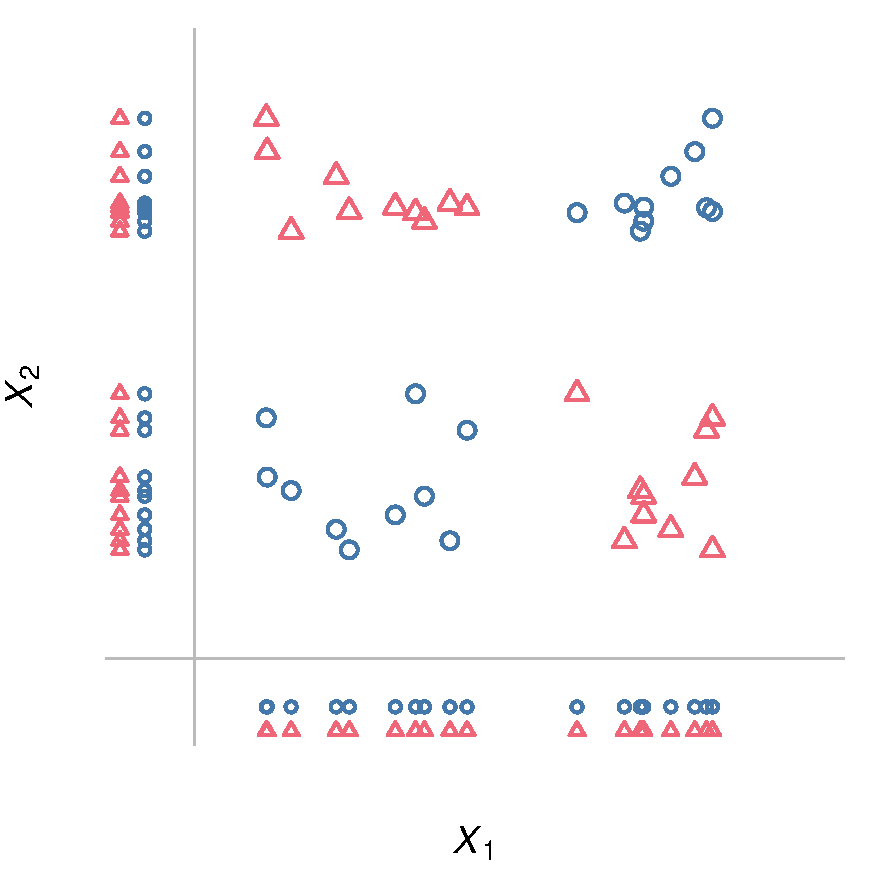
\includegraphics[width=\linewidth]{example_importance_context3.pdf}%
% \includegraphics[width=\linewidth]{baseratetrials.png}\\[\jot]
% \includegraphics[width=\linewidth]{baseratepopulation.png}
\end{wrapfigure}%
To answer this general question, which is too vague (ill-posed), we must first specify which other predictors the predictor of interest is used with, and what we mean by \enquote{important}.

The schematic picture on the side illustrates the necessity of specifying a predictor's context. Individuals in this population can be either \textcolor{bluepurple}{blue circles $\circ$} or \textcolor{redpurple}{red triangles $\triangle$} and have two predictors $X_{1}, X_{2}$. Predictor $X_{1}$, if used by itself, is worthless in distinguishing the two subpopulations, because these have identical marginal distributions (depicted beside the grey lines). If used in conjunction with $X_{2}$, however, predictor $X_{1}$ allows us to identify an individual's subpopulation with full certainty. It is therefore an essential predictor in this case: dropping it would lead to a complete loss of predictive power. An analogous discussion holds for $X_{2}$ in the present case. The converse can also happen (not illustrated): a predictor might be \enquote{good} if used by itself, and yet it might be discarded without any loss if used in combination with others.

A predictor's \enquote{importance} or \enquote{prognostic power} is undefined until we specify a relevant metric, for predictors can be ranked differently by different metrics. From our discussion so far it should be clear that in clinical decision-making the canonical metric is the \emph{utility} which a predictor's presence or absence leads to. This point was partially illustrated with Curtis's example in the previous subsection. What if we want to make an assessment, not for a single patient, but for full population? It can be proved, again from decision-theoretic principles, that the population average of all utility matrices should be used in this case \citep[\cf][\sect~4.1]{dyrlandetal2022}. This seems a quantity very difficult to assess; but it can also be proved that even just a semi-quantitative assessment leads to better results than using some other \enquote{general-purpose} metric \citep[\sect~4.2]{dyrlandetal2022}.

The \ljm\ allows us to compute the expected value of virtually any prognostic-importance metric of any subset of predictors available in the dataset. Two facts of paramount advantage are that (a) \emph{the prognostic power of a set of predictors found with the \ljm\ is the maximal one obtainable by \textbf{any} inference algorithm}, or in other words it is an intrinsic property of that set of predictors; (b) \emph{the \ljm\ achieves this maximal power}. Thus, if the \ljm\ says that the accuracy obtainable with a given set of predictors is 70\%, then we know that no other inference algorithm of any kind can reach a higher accuracy than 70\%; inference algorithms that reach lower accuracy can in principle be improved upon. The \ljm, by construction, will reach this accuracy.

We illustrate this kind of computation in our example case, using: (a) two metrics, the accuracy and the mutual information~\citep{shannon1948,coveretal1991_r2006} between a set of predictors and the event of conversion to \ad; and (b) 27 different sets of predictors:
\begin{itemize}
\item every predictor, used individually (12 sets);
\item all cognitive-test predictors used together, jointly with demographic information (\age and \sex);
\item \apoe, Hippocampal Volume, and demographic information, used together;
\item all predictors together minus one, excluding each single predictor in turn (12 sets);
\item all predictors jointly.
\end{itemize}

Use of the accuracy assumes that the population of patients has only two available treatments having average utility matrix $\bigl[\begin{smallmatrix}1&0\\0&1\end{smallmatrix}\bigr]$. Mutual information is a model-free measure of the relation between two sets of variates, with diverse operational interpretations \citep{mackay1995_r2005,woodward1953_r1964,minka1998d_r2003,goodetal1968,kelly1956,kullback1959_r1978} and international standards \citep{iso2008c}. A set of predictors and a binary variate (such as our conversion to \ad) have a mutual information of $1\,\mathrm{Sh}$ if and only if there is a non-constant deterministic function from the former to the latter. \mynotew{Consider using conditional entropy instead of mutual info; maybe both. Show the distribution of cAD/sMCI across the main diagonal o f the 12D predictor space}

Our specific questions are the following: \enquote{What is the expected value of the accuracy for the next new patient, if we use the given set of predictors?} and \enquote{What is the mutual information between the given set of predictors and the predictand, given the present available data?}.

The answers to these questions are reported in \fig~\ref{fig:mutual_info}, ordered from bottom to top according to increasing metric. The ordering of mutual information and accuracy agree within the uncertainty of the numerical computation (Monte Carlo integration). The latter is reported as coverage intervals of $\pm$~two standard deviations.
\begin{figure}[!t]% with figure
  \centering%
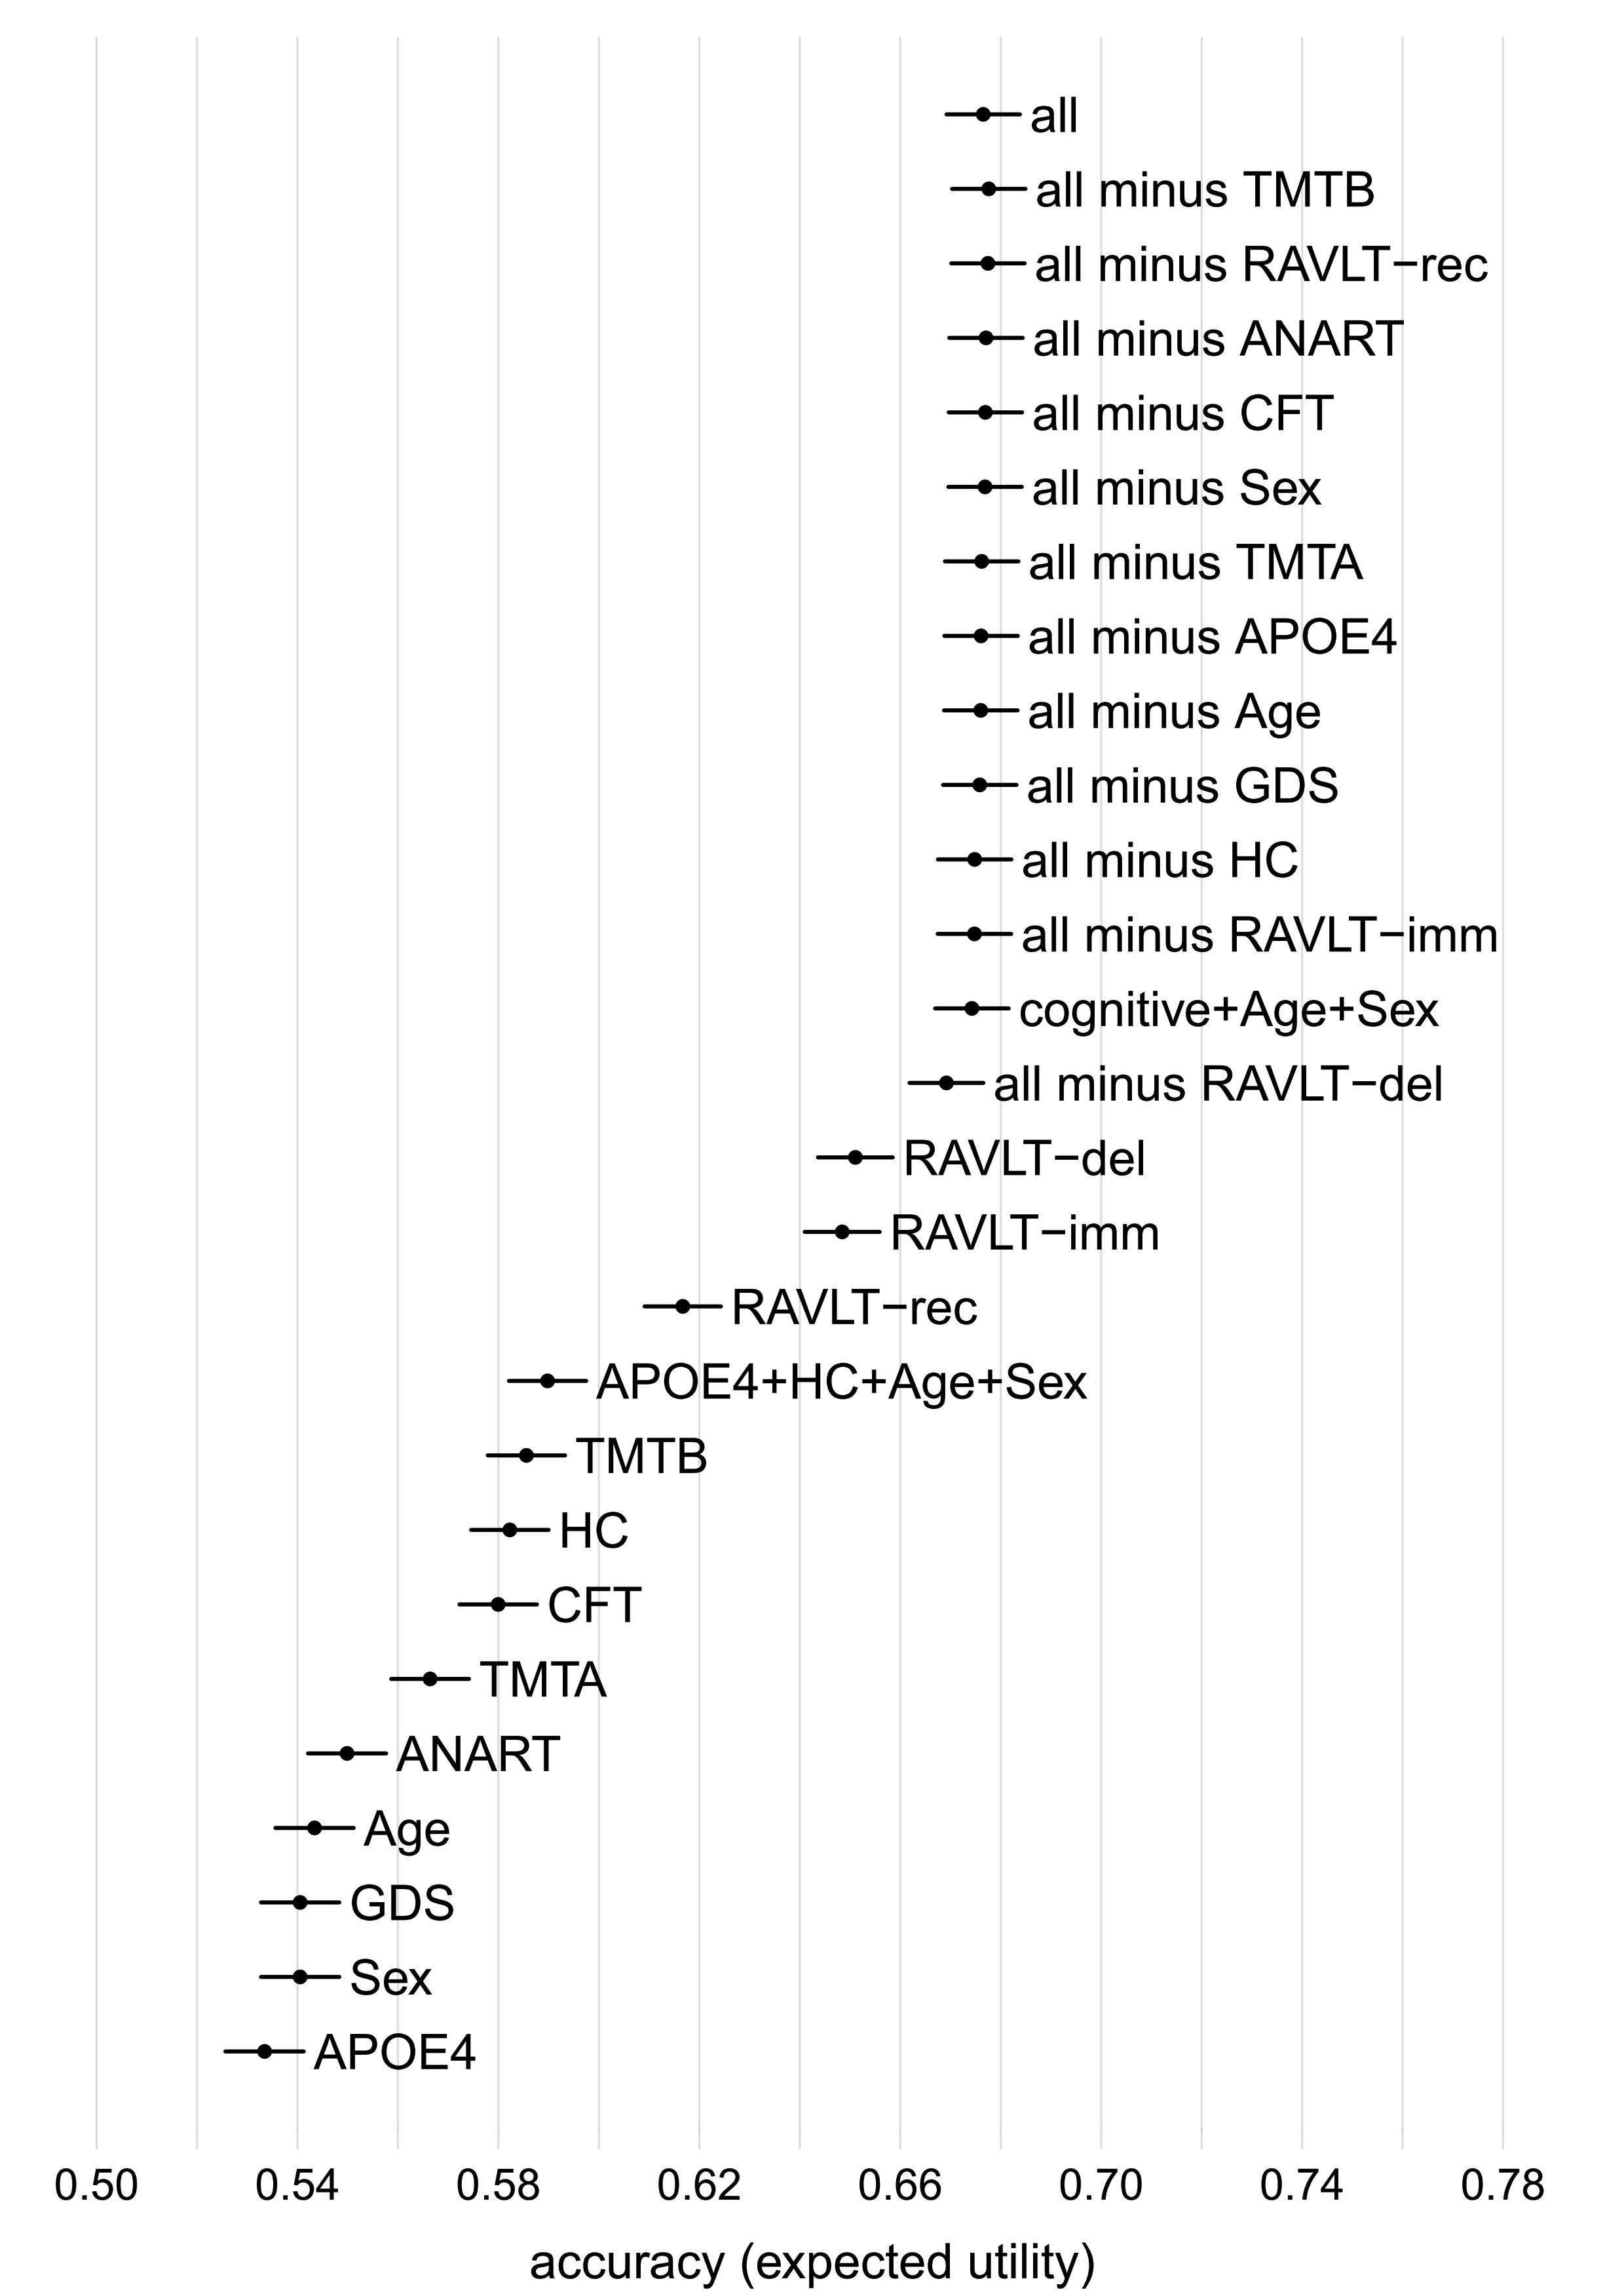
\includegraphics[width=0.494\linewidth]{accuracy_ranks.pdf}%
\hfill%
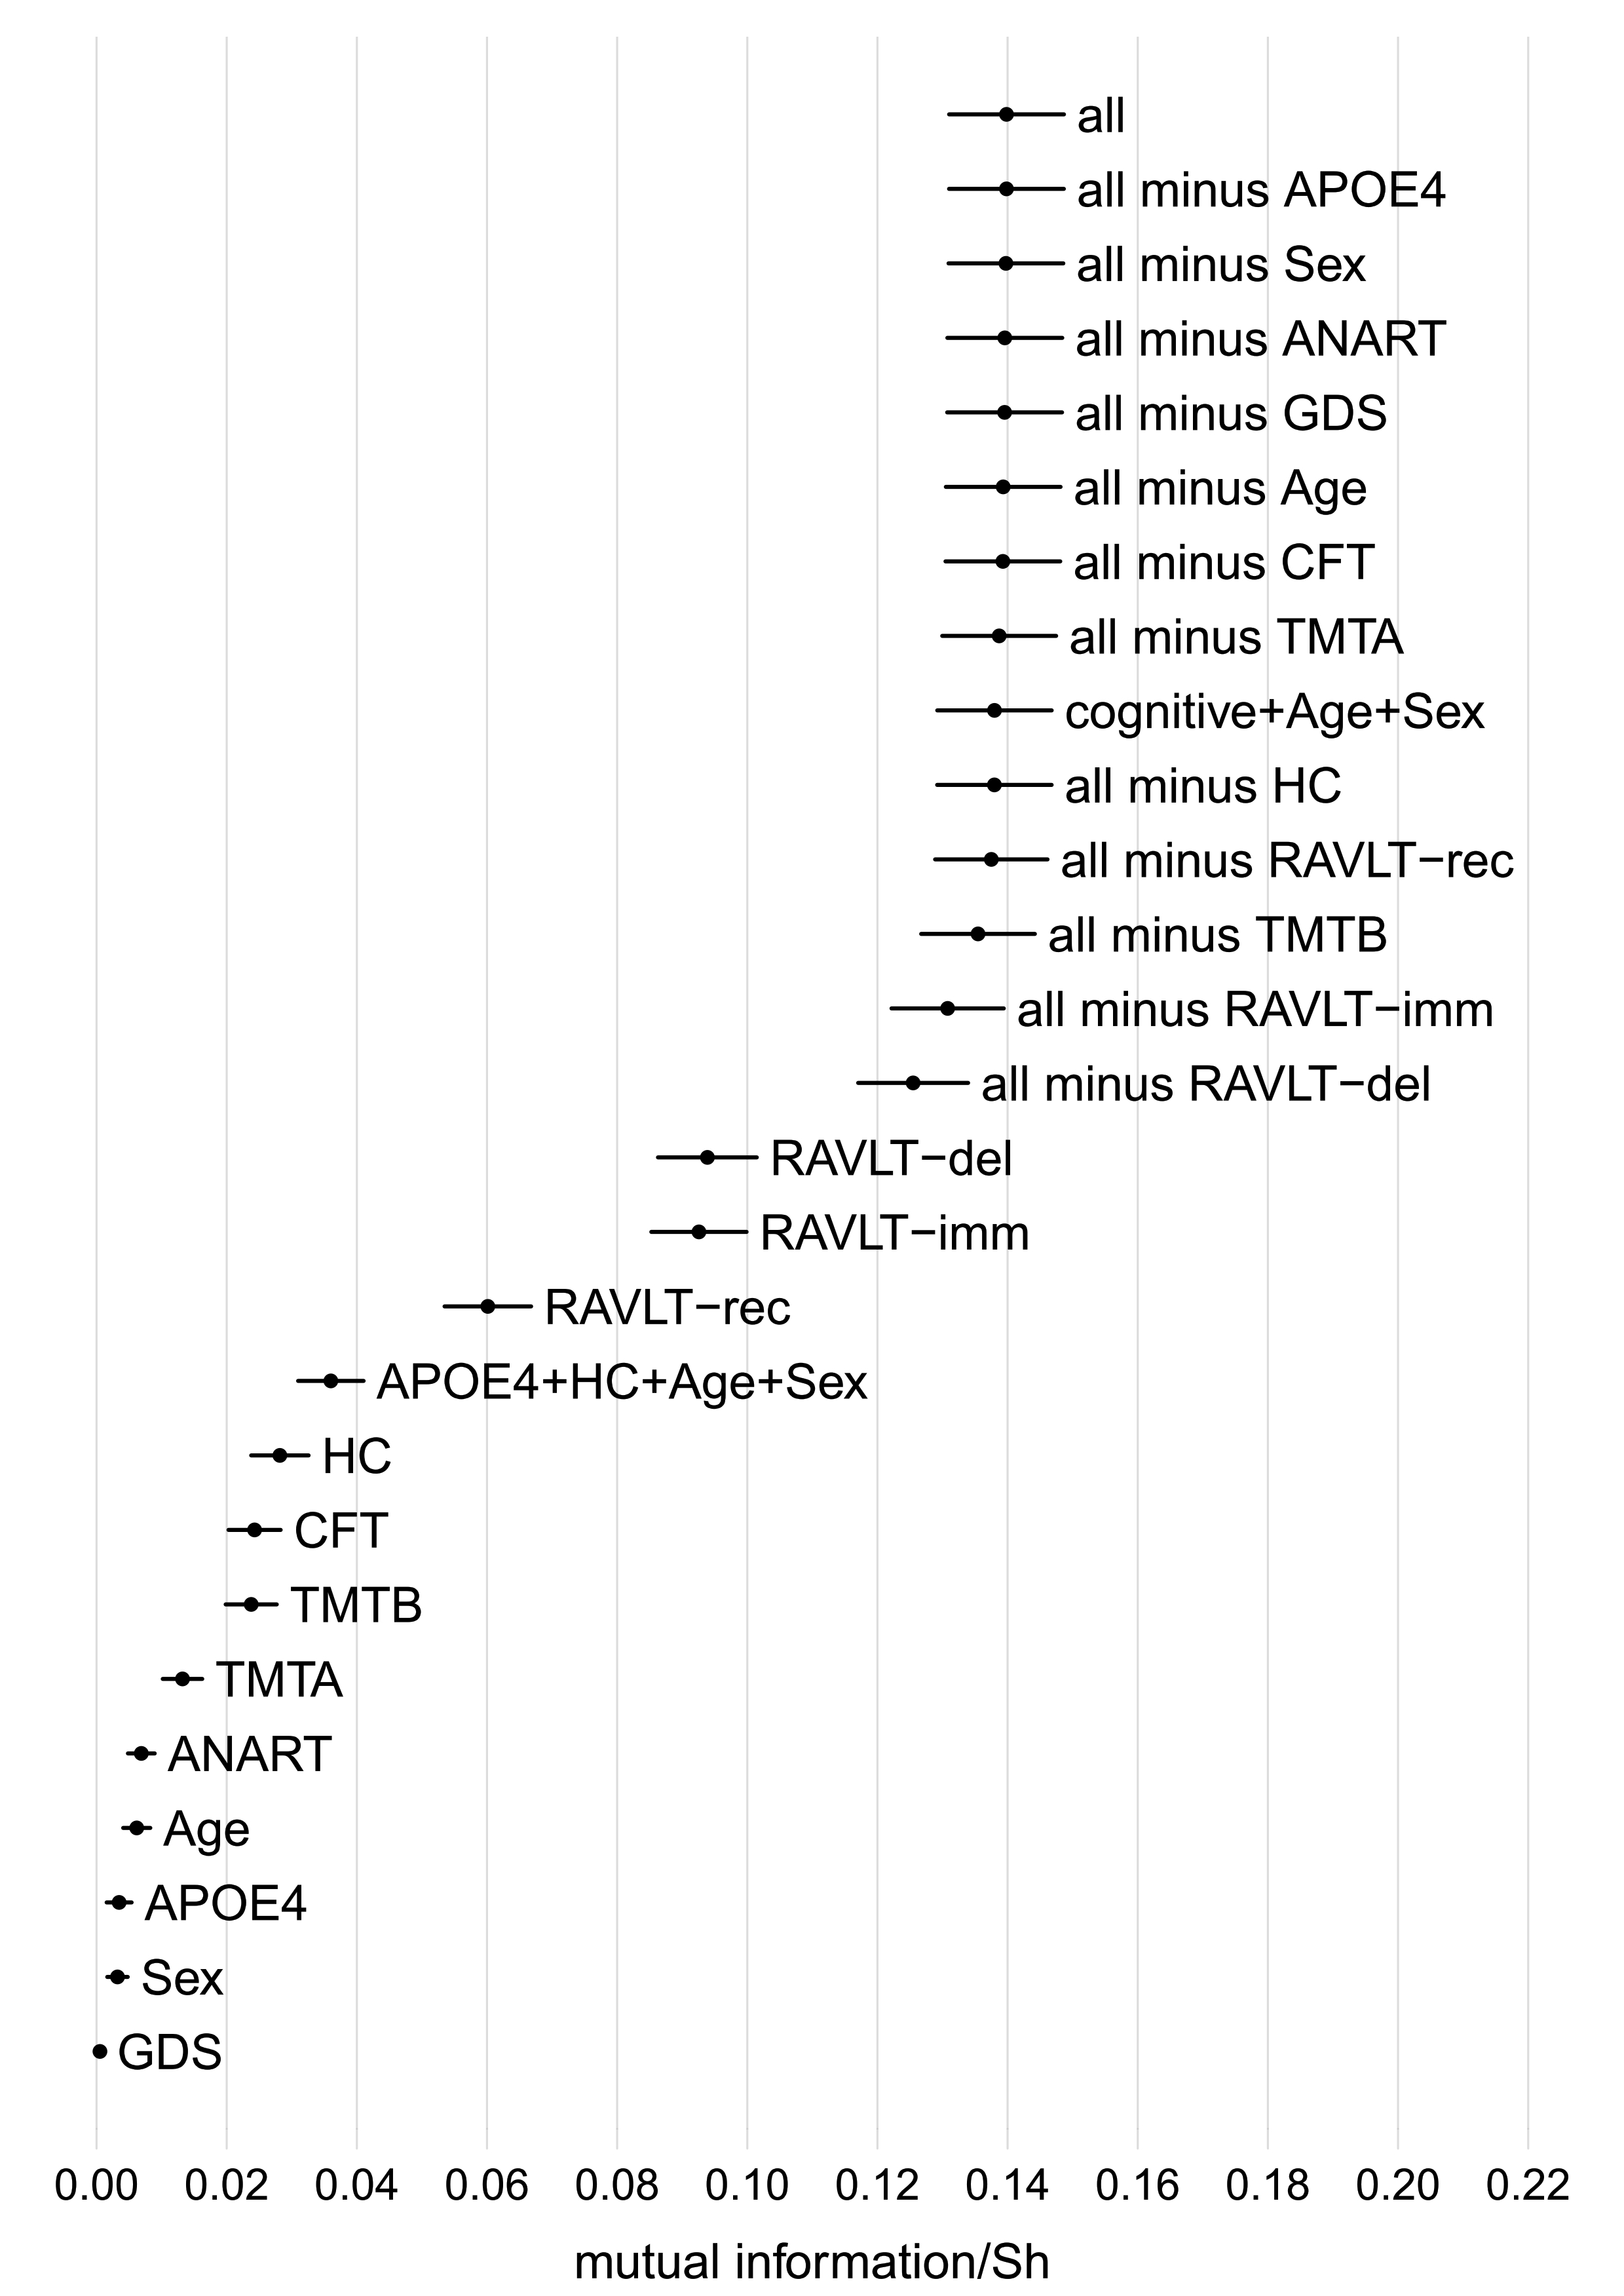
\includegraphics[width=0.494\linewidth]{MI_ranks.pdf}%
\caption{Expected accuracy (for the next new patient) and mutual information of several sets of predictors for the prognosis of conversion to \ad. Both graphs have been vertically ordered according to increasing values; the two rankings agree within the respective uncertainties. The \texttt{all} predictor set is mathematically guaranteed to be optimal according to both metrics, and has therefore be ranked first. Bars show the uncertainty interval ($\pm$~two standard deviations).}\label{fig:mutual_info}
\end{figure}%


The figure reveals several interesting findings, \emph{valid within the population selected for the dataset}, which can be compared with the analysis in  \citet[see especially Fig.~3 and Table~3]{ryeetal2022}:
\begin{itemize}
\item The set of 12 predictors considered in the present work \citep[and in ][]{ryeetal2022} can at most lead to a prognostic accuracy of around 68\%, for any inference algorithm. This fact agrees with the (completely independent) findings in \citet{ryeetal2022}, where a maximal accuracy of 68\% was found using an ensemble model; the present analysis also shows that that model managed to achieve the maximal accuracy possible with these predictors (but see \sect~\ref{sec:discussion} for limitations of that model.)
\item \apoe, \gds, \age, \sex, and to some degree \anart are poor predictors (within this population), when used alone and when used in combination with all other predictors. The latter point is evident from the fact that the mutual information of the combined predictors barely decrease if any one of these four predictors is omitted.
\item The combined cognitive and demographic variates are better predictors than the combined hippocampal, \apoe, and demographic variates.
\item \ravltimm, \ravltdel, and to a lesser degree are good predictors, both when used alone and when used in combination with all other predictors. Hippocampal Volume is a poorer predictor than any of the \texttt{RAVLT} when used alone, and likely also when used in combination with all others \citep[contrast this with][]{ryeetal2022}.
\end{itemize}

The \ljm\ shows that the omission of any one of the 12 predictors, except \ravltdel and possibly \ravltimm, does not lead to an appreciable decrease in accuracy (relative decrease of 0.3\% or less) or in mutual information (relative decrease of less than 3\%). This puts the importance analysis of \citet{ryeetal2022} into perspective. The exact quantification of these subtle differences is computationally quite expensive and we did not carry it out further.


% \begin{table}[!t]
%   \centering
%   \begin{tabular}{ll}
%     \hline\\[-1.5\jot]
%     {\small predictor set} &{\small mutual information/Sh}
%     \\[\jot]
% GDS               &0.0005  \\
% Sex               &0.0032  \\
% APOE4                    &0.0035  \\
% Age                       &0.006  \\
% ANART            &0.006  \\
% TMTA            &0.013  \\
% TMTB            &0.023  \\
% CFT           &0.024  \\
% HC              &0.028  \\
% \textbf{APOE4 + HC + demographic}         &0.036  \\
% RAVLT-rec            &0.060  \\
% RAVLT-imm           &0.092  \\
% RAVLT-del          &0.094  \\
% all minus RAVLT-del &0.125  \\
% all minus RAVLT-imm  &0.131  \\
% all minus TMTB   &0.135  \\
% \textbf{cognitive + demographic}            &0.138  \\
% all minus RAVLT-rec   &0.138  \\
% all minus HC     &0.138  \\
% all minus TMTA   &0.139  \\
% all minus CFT  &0.139  \\
% all minus Age              &0.139  \\
% all minus GDS      &0.140  \\
% all minus ANART   &0.140  \\
% all minus Sex      &0.140  \\
% all minus APOE4           &0.140  \\
% \textbf{all}                       &0.140  \\[\jot]
%     \hline 
%   \end{tabular}
%   \caption{Mutual information between various predictor sets and conversion to \ad. The mutual information is measured in shannons and has a maximum numerical error of $0.004\,\mathrm{Sh}$}\label{tab:mutual_info}
% \end{table}


\bigskip% Newpage break just to help while writing the draft
\subsection{Summary of the case study}
\label{sec:summary}


Summary in table~\ref{tab:summary}.

\begin{table}[!t]
  \centering
  \begin{tabular}{lcccc}
    &{\small Olivia} &{\small Ariel} &{\small Bianca} &{\small Curtis}
    \\[\jot]
    \hline\\[-1.5\jot]
    \emph{\small Predictor values}&&&& \\[\jot]
    \age&75.4&75.4&75.4&\textcolor{redpurple}{63.8} \\
    \sex&F&F&F&\textcolor{redpurple}{M} \\
    \hv${}/10^{-3}$&4.26&4.26&4.26&\textcolor{redpurple}{[missing]} \\
    \apoe&N&N&N&\textcolor{redpurple}{Y} \\
    \anart&18&18&18&\textcolor{redpurple}{15} \\
    \cft&21&21&21&\textcolor{redpurple}{14} \\
    \gds&3&3&3&\textcolor{redpurple}{2} \\
    \ravltimm&36&36&36&\textcolor{redpurple}{20} \\
    \ravltdel&5&5&5&\textcolor{redpurple}{0} \\
    \ravltrec&10&10&10&\textcolor{redpurple}{3} \\
    \tmta&21&21&21&\textcolor{redpurple}{36} \\
    \tmtb&114&114&114&\textcolor{redpurple}{126}
    \\[2\jot] \hline\\
    \emph{\small Additional information, final probability}&&&& \\[\jot]
    {\small auxiliary info}&
    {\small none}&
    {\small\color{redpurple} family history, base rate}&
    {\small none}&
    {\small none}\\
    {\small applicable dataset statistics}&
    {\small all}&
    {\small\color{redpurple} predictor$\|$predictand}&
    {\small all}&
    {\small all}\\
    {\small prior probability of conversion}&
    0.463&\textcolor{redpurple}{0.65}&0.463&0.463
    \\[2\jot] \hline\\
    \emph{\small Available actions and utilities}&&&& \\[\jot]
    $
    \begin{matrix}
      &\begin{smallmatrix}\nAD&\AD\end{smallmatrix}\\
      \begin{smallmatrix}
      \text{treatment $\alpha$}\\
      \text{treatment $\beta$}\\
      \text{treatment $\gamma$}\\
      \text{treatment $\delta$}
    \end{smallmatrix}&
    \Biggl[\begin{smallmatrix}
      \hphantom{\nAD}&\hphantom{\AD}\\&\\&\\&
    \end{smallmatrix}\Biggr]
    \end{matrix}$
    &
    $\begin{bmatrix}10&0\\9&3\\8&5\\0&10\end{bmatrix}$
    &
    $\begin{bmatrix}10&0\\9&3\\8&5\\0&10\end{bmatrix}$
    &
    $\color{redpurple}\begin{bmatrix}10&0\\8&3\\7&5\\0&10\end{bmatrix}$
    &
    $\begin{bmatrix}10&0\\9&3\\8&5\\0&10\end{bmatrix}$
    \\[4\jot] \hline\\
    \emph{\small Outputs of \ljm}&&&& \\[2\jot]
    {\small $\p(\AD \| \text{predictors})$}&
    0.302&0.302&0.302&0.703
    \\
    {\small $\p(\text{predictors} \| \AD)/10^{-12}$}&
    8.97&8.97&8.97&1.14
    \\
    {\small $\p(\text{predictors} \| \nAD)/10^{-12}$}&
    18.6&18.6&18.6&0.343
    \\[\jot]
    {\small final probability of conversion}&
    0.302&0.47&0.302&0.703
    \\[\jot]
    $\begin{matrix}
      \text{exp. utility treatment }\alpha\\ 
      \text{exp. utility treatment }\beta\\ 
      \text{exp. utility treatment }\gamma\\ 
      \text{exp. utility treatment }\delta\\[2\jot]
      \text{Optimal treatment}
    \end{matrix}$
    &
    $\begin{matrix}6.98\\\bm{7.19}\\7.09\\3.02\\[2\jot]\bm{\beta}\end{matrix}$
    &
    $\begin{matrix}5.27\\6.16\\\bm{6.58}\\4.73\\[2\jot]\bm{\gamma}\end{matrix}$
    &
    $\begin{matrix}\bm{6.98}\\6.49\\6.40\\3.02\\[2\jot]\bm{\alpha}\end{matrix}$
    &
    $\begin{matrix}2.97\\4.78\\5.89\\\bm{7.03}\\[2\jot]\bm{\delta}\end{matrix}$
    \\[6\jot]
    \hline
  \end{tabular}
  \caption{\mynotep{Summary. The basic data that distinguish Ariel, Bianca, Curtis from Olivia are in \textcolor{redpurple}{red}.}}\label{tab:summary}
\end{table}



\bigskip% Newpage break just to help while writing the draft
\section{Discussion}
\label{sec:discussion}

\mynotew{[Luca] There are a couple different ways to introduce the discussion. I'll write some variants as soon as possible}

The differences among patients which are relevant to clinical diagnosis/prognosis and decision-making can be approximately divided into three categories:
\begin{enumerate}[I.]
\item\label{item:diff_corepredictors} differences in the availability and values of a core set of clinical predictors, for which we have population-wide statistical information;
\item\label{item:diff_priorinfo} differences in the availability and values of auxiliary and usually \enquote{softer} predictors, such as geographical or family background; or more generally of predictors not belonging to the core set;
\item\label{item:diff_utility} differences in the availability and benefit of clinical courses of actions, such as treatments and further tests.
\end{enumerate}

These differences are intimately connected with, and partially stem from, several hallmarks of a clinician's tasks:

First, there is often an irreducible element of uncertainty in inferring a medical or biological condition from a set of predictors. In mathematical terms, there is no function from predictors to predictands \mynotep{refer to a figure in the previous sections}. This is especially often the case for predictors that are more readily available and less invasive, and therefore more desirable. The irreducible uncertainty originates from the natural variability within a population. Yet this variability can be harnessed, and the way to harness it can crucially vary from patient to patient. We illustrated this with an example in the inset of \sect~\ref{sec:population_step}, p.~\pageref{tab:superiority_predictors_given_predictand}, which showed that any relation from predictors to predictands lead to poor prognoses, whereas taking into account the variability in the predictors \emph{given} the predictand improved our prognoses.

Second, owing to the irreducible prognostic uncertainty, the clinician's ultimate task is not one of classification or regression, but one of \emph{decision-making under risk}. This is clear if we consider that a clinician may have \emph{three or more} courses of action to choose from, even if the unknown medical condition only has \emph{two} possible \enquote{class labels}. A pure class label is therefore of no help to the clinician, who instead needs to know the uncertainty or probability of the label, in order to evaluate risks and benefits, and from these make a final decision. The choice of a course of action is moreover the moment were patient differences can be very dramatic.

\mynotep{to be finished}


% Current development of prognostic methods, especially when based on machine learning, is almost exclusively focused on differences in the first category. Moreover, in presenting how these methods could be applied, the clinical context is usually overly simplified, as if it were just a simple classification task. It is not. The clinician's ultimate goal is not to \enquote{classify} a patient's condition -- a clinician doesn't simply say \enquote{hey, you're likely to develop Alzheimer. Goodbye, now you can go!}. The ultimate goal is to choose among several courses of action. And the number of such courses of action is typically larger than the number of possible \enquote{labels} of the medical condition. Already this simple numerical discrepancy shows that classification methods don't fill the bill. \mynotep{to be continued...}

\mynotep{Possible additional point of view} Let's assume that current technology allows for a particular maximal rate of extraction of information per unit time, and if we assume that different inference algorithms reach this maximum rate (or do not reach it by a common amount). Information and communication theory \citep[I--II]{mackay1995_r2005} then suggests that if one inference algorithm is, say 100 times faster than a \ljm, its output has also 100 times less information than a \ljm's. Do we need this extra information? The example case illustrated in the present work shows that part of this extra information is necessary for personalized medicine; and the remaining amount can be very useful or at times necessary for sensitivity analyses or resource planning.

\subsection{Counters to critiques}
\label{sec:critics}

Any inference or decision-making algorithm aspiring to take into account patient differences must perforce have some open \enquote{input slots} for such differences. We saw that the \ljm\ requires inputs about a patient's specific predictors, relevant statistical relations and auxiliary data, and treatment utilities.

Some researchers may wonder: can such additional input be avoided? They fear that errors could sneak in through these extra inputs.

This question is answered by a mathematical theorem at the very core of decision theory \footnote{\citet{savage1954_r1972,luceetal1957,raiffaetal1961_r2000,atkinsonetal1964,ferguson1967,lindley1971_r1988,kreps1988,bernardoetal1994_r2000,prattetal1995_r1996,lindley2006_r2014,pettigrew2011_r2019}}, which is too seldom emphasized: Any decision we make, either (A) comes explicitly or implicitly through some set of utilities and maximization of their expectations, or (B) is logically inconsistent. There is no third alternative. Thus the choice is not between using utilities or not using utilities, but between choosing them explicitly or letting them be chosen in a way we don't know. If you use a decision-making algorithm that does not ask you for utilities, then the algorithm is internally supplying utilities beyond your control (and probably divorced from your specific problem), or worse, is committing logical inconsistencies.

The first advantage of explicitly operating through utilities, probabilities, decision theory, is that we are at the very least sure of not acting in a self-contradictory way. The second advantage is that the utilities used to arrive at a decision lie openly in front of us. We can analyse and change them if we find them inappropriate to a specific problem. If they are hidden, it's more difficult to analyse which are inappropriate and how they should be changed.

\mynotep{Subtly hidden disastrous consequences of not following normative decision theory: An algorithm can lead to saving 85\,000 patients out of 100\,000 and be deemed a success. But if the ideal algorithm had been used, 95\,000 patients would actually have been saved. What shall we say to the families of the 10\,000 patients who could have been saved but weren't?}

\subsection{Range of application of \ljm s}
\label{sec:rangeLJM}

The range of application of the \ljm\ used in the present study has two kinds of bound: computational and theoretical.

As mentioned in \sect~\ref{sec:predictor_step} and explained in appendix~\ref{sec:maths_tjm}, the fact that the \ljm\ extracts all available information from the dataset also makes it computationally expensive. It is at present impossible to use with high-dimensional predictors (if our dataset had included a predictor such as a $128\times128\times128$ grayscale MRI image, the learning stage would have taken around 100 years). Approximate but much faster algorithms such as neural networks and random forests are thus, at present, still the only options with such predictors. There is, however, the interesting possibility of combining such fast algorithms together with a \ljm, as a post-processor of their raw output. This allows us to extract useful information usually hidden in such output at a low computational cost \citep{dyrlandetal2022b}. Such information can be then used for clinical decision making as illustrated in the present work.

As explained in \sect~\ref{sec:population_step}, the essentially sole assumption underlying the \ljm's inference and its practical used with new patients, is that the latter can be assumed to come, at least in some respects, from the same population as the learning dataset (in technical jargon, partial or conditional exchangeability applies). This precludes using the \ljm\ to forecast how the statistics of the full population could change in the future. However, the machine can be used for time-dependent (transversal \mynotez{correct?}) inferences within a stable population, such as forecasts of the future time of disease onset, expected lifelength, and similar. For example, if data about the time of conversion to \ad\ were available in the dataset, the \ljm\ could forecast not only \emph{whether}, but also \emph{when} the conversion could take place \citep[\cf\ \eg][]{delacruzmesiaetal2007}.


\bigskip% Newpage break just to help while writing the draft
\appendix
\renewcommand\thesection{\Alph{section}}
\section{Appendices}
\label{sec:appendices}


% \subsection{Predictors and predictand}
% \label{sec:predictors_description}

% For the present study, data used in the learning stage of \sect~\ref{sec:learn_application} comes from the Alzheimer's Disease Neuroimaging Initiative (\adni) study. This longitudinal multicenter study is designed to develop and validate neuroimaging and biochemical biomarkers for early detection, monitoring, and treatment of Alzheimer's disease \citep{petersenetal2010}. The present sample of 704 subjects consisted of all \adni\ participants meeting the criteria for Mild Cognitive Impairment at their first, baseline assessment who additionally had a minimum of three study visits (that is, baseline visit and at least two additional visits), and three MRI examinations. A reevaluation of each subject's diagnostic status was conducted at each study visit, and this longitudinal diagnostic label was used to partition our sample into 325 subjects converting to Alzheimer's Disease following the first study visit, and 379 subjects remaining stable with \mci. Criteria used for classifying subjects as having \mci\ and \ad, as well as \adni's general criteria for subject inclusion, are described in \citet{mckhannetal1984,petersenetal2010}.

\subsection{Mathematical details about the \ljm}
\label{sec:maths_tjm}

% \setlength{\intextsep}{0ex}% with wrapfigure
% \setlength{\columnsep}{1ex}% with wrapfigure
% \begin{wrapfigure}{r}{0.25\linewidth}% with wrapfigure
% %\vspace{-1ex}%
% \includegraphics[width=\linewidth]{noisedistrnolines.pdf}%
% \end{wrapfigure}%
% The space of possible full-population frequency distributions has finite (owing to the finite precision of measurements) but very large number of dimensions. For our dataset it is around the order of $10^{20}$. Most distributions in such space, however, look like noise, as the example on the side, and are completely unrealistic as distributions for a \emph{full population}.

As discussed in \sect~\ref{sec:predictor_step}, the \ljm\ explores the space of possible distributions of frequencies of all 13 variates listed in table~\ref{tab:patients_data}, for the full population of patients from which the dataset originates. In the present study it does so by using a total of 1535 independent parameters to represent the distributions, with roughly 190 parameters for each continuous or integer variate. As a crude intuition, it is as if we divided the range of each variate into 190 bins, and considered all possible frequency histograms over these. The actual parametrization is smarter, using parameters to represent less and less smooth traits of the distribution. We indeed expect the distribution for a full population to have some degree of smoothness, owing to physical and biological reasons. Actually, the number of parameters used is in principle infinite, because the machine gives a warning if the data indicates that more parameters are needed. In the present study the data indicates, on the contrary, that fewer than 250 parameters would be enough. More details on the mathematical representation can be found in \citet{dunsonetal2011}; see also \citet{rossi2014,rasmussen1999}.

\mynotep{Should I add a more precise description of the mathematical representation?}

\mynotep{Is the part below superfluous? I think it could be interesting for readers from machine learning}

There is a fundamental difference in how the \ljm\ and most popular machine-learning algorithms (including neural networks, random forests, support-vector machines, excluding gaussian processes) work. The latter do, at bottom, an optimization, looking for the minimum of some error function. The \ljm\ does a full \emph{space exploration} and \emph{averaging}, as explained in \sect~\ref{sec:predictor_step}. Inference and generalization in fact essentially rely on averaging operations in problems such as the present one \citetext{\citealt{definetti1930,definetti1937,dawid2013}; \citealt[\sects~4.2--4.3]{bernardoetal1994_r2000}; see also \citealt{selfetal1987}}. The optimization done by most machine-learning algorithms is an approximate form of averaging -- assuming or hoping that most of the mass to be averaged is around the extremum \citep[\chap~16]{mackay1992,murphy2012}. But the underlying necessity of a proper averaging becomes manifest in many of the obligatory procedures that go together with training a machine-learning algorithm; cross-validation for instance \citep{mackay1992b}. \mynotew{Add note: \enquote{ensembling} in ML is not this kind of averaging \citep[\sect~18.2]{murphy2022}}

This difference explains why the \ljm\ is computationally much more expensive than other algorithms, but also why its output is informationally so rich, and why it does not need any validation datasets, test datasets, other data splits, or cross-validation procedures (it can be proved that one of the internal computations of the machine is mathematically equivalent to doing $k$-fold cross-validations for \emph{all possible} data splits and $k$; see \eg\ \citealt{portamana2019b,fongetal2020}).

\mynotep{one more remark about extremum-search being equivalent to making a choice, but the utilities are not controlled by the patient and not flexible.}


\subsection{Computational details}
\label{sec:comput_details}

The learning stage, with 13 variates and 704 datapoints, took less than 5~hours. The computation was done with 16 parallel 3.0--4.80~GHz cores. After that, calculation of probabilities and expected utilities for any single patient is immediate. The mutual information and accuracy analysis of \sect~\ref{sec:additional_results} took roughly 1~h.










%%\setlength{\intextsep}{0ex}% with wrapfigure
%%\setlength{\columnsep}{0ex}% with wrapfigure
%\begin{figure}[p!]% with figure
%\begin{wrapfigure}{r}{0.4\linewidth} % with wrapfigure
%  \centering\includegraphics[trim={12ex 0 18ex 0},clip,width=\linewidth]{maxent_saddle.png}\\
%\caption{caption}\label{fig:comparison_a5}
%\end{figure}% exp_family_maxent.nb




\newpage
\hrule
\hrule



% {\color{yellow}\tiny For Original Research Articles \citep{conference}, Clinical Trial Articles \citep{article}, and Technology Reports \citep{patent}, the introduction should be succinct, with no subheadings \citep{book}. For Case Reports the Introduction should include symptoms at presentation \citep{chapter}, physical exams and lab results \citep{dataset}.

% }



% \section{Article types}

% For requirements for a specific article type please refer to the Article Types on any Frontiers journal page. Please also refer to  \href{http://home.frontiersin.org/about/author-guidelines#Sections}{Author Guidelines} for further information on how to organize your manuscript in the required sections or their equivalents for your field

% % For Original Research articles, please note that the Material and Methods section can be placed in any of the following ways: before Results, before Discussion or after Discussion.

% \section{Manuscript Formatting}

% \subsection{Heading Levels}

% %There are 5 heading levels

% \subsection{Level 2}
% \subsubsection{Level 3}
% \paragraph{Level 4}
% \subparagraph{Level 5}

% \subsection{Equations}
% Equations should be inserted in editable format from the equation editor.

% \begin{equation}
% \sum x+ y =Z\label{eq:01}
% \end{equation}

% \subsection{Figures}
% Frontiers requires figures to be submitted individually, in the same order as they are referred to in the manuscript. Figures will then be automatically embedded at the bottom of the submitted manuscript. Kindly ensure that each table and figure is mentioned in the text and in numerical order. Figures must be of sufficient resolution for publication \href{https://www.frontiersin.org/about/author-guidelines#ImageSizeRequirements}{see here for examples and minimum requirements}. Figures which are not according to the guidelines will cause substantial delay during the production process. Please see \href{https://www.frontiersin.org/about/author-guidelines#FigureRequirementsStyleGuidelines}{here} for full figure guidelines. Cite figures with subfigures as figure \ref{fig:Subfigure 1} and \ref{fig:Subfigure 2}.


% \subsubsection{Permission to Reuse and Copyright}
% Figures, tables, and images will be published under a Creative Commons CC-BY licence and permission must be obtained for use of copyrighted material from other sources (including re-published/adapted/modified/partial figures and images from the internet). It is the responsibility of the authors to acquire the licenses, to follow any citation instructions requested by third-party rights holders, and cover any supplementary charges.
% %%Figures, tables, and images will be published under a Creative Commons CC-BY licence and permission must be obtained for use of copyrighted material from other sources (including re-published/adapted/modified/partial figures and images from the internet). It is the responsibility of the authors to acquire the licenses, to follow any citation instructions requested by third-party rights holders, and cover any supplementary charges.

% \subsection{Tables}
% Tables should be inserted at the end of the manuscript. Please build your table directly in LaTeX.Tables provided as jpeg/tiff files will not be accepted. Please note that very large tables (covering several pages) cannot be included in the final PDF for reasons of space. These tables will be published as \href{http://home.frontiersin.org/about/author-guidelines#SupplementaryMaterial}{Supplementary Material} on the online article page at the time of acceptance. The author will be notified during the typesetting of the final article if this is the case. 

% \section{Nomenclature}

% \subsection{Resource Identification Initiative}
% To take part in the Resource Identification Initiative, please use the corresponding catalog number and RRID in your current manuscript. For more information about the project and for steps on how to search for an RRID, please click \href{http://www.frontiersin.org/files/pdf/letter_to_author.pdf}{here}.

% \subsection{Life Science Identifiers}
% Life Science Identifiers (LSIDs) for ZOOBANK registered names or nomenclatural acts should be listed in the manuscript before the keywords. For more information on LSIDs please see \href{https://www.frontiersin.org/about/author-guidelines#Nomenclature}{Inclusion of Zoological Nomenclature} section of the guidelines.


% \section{Additional Requirements}

% For additional requirements for specific article types and further information please refer to \href{http://www.frontiersin.org/about/AuthorGuidelines#AdditionalRequirements}{Author Guidelines}.

\section*{Conflict of Interest Statement}
%All financial, commercial or other relationships that might be perceived by the academic community as representing a potential conflict of interest must be disclosed. If no such relationship exists, authors will be asked to confirm the following statement: 

The authors declare that the research was conducted in the absence of any commercial or financial relationships that could be construed as a potential conflict of interest.

\section*{Author Contributions}

The authors were too immersed in the development of the present work to keep a detailed record of who did what.

% The Author Contributions section is mandatory for all articles, including articles by sole authors. If an appropriate statement is not provided on submission, a standard one will be inserted during the production process. The Author Contributions statement must describe the contributions of individual authors referred to by their initials and, in doing so, all authors agree to be accountable for the content of the work. Please see  \href{https://www.frontiersin.org/about/policies-and-publication-ethics#AuthorshipAuthorResponsibilities}{here} for full authorship criteria.

\section*{Funding}
Details of all funding sources should be provided, including grant numbers if applicable. Please ensure to add all necessary funding information, as after publication this is no longer possible.

\section*{Acknowledgments}
PGLPM thanks Soledad Gonzalo Cogno and Iv\'an Davidovich for inspiring discussions;
Mari, Miri, Emma for continuous encouragement and affection; Buster Keaton and Saitama for filling life with awe and inspiration; and the developers and maintainers of Nimble, \LaTeX, Emacs, AUC\TeX, Open Science Framework, R, Inkscape, LibreOffice, Sci-Hub for making a free and impartial scientific exchange possible.

\section*{Supplemental Data}
 \href{http://home.frontiersin.org/about/author-guidelines#SupplementaryMaterial}{Supplementary Material} should be uploaded separately on submission, if there are Supplementary Figures, please include the caption in the same file as the figure. LaTeX Supplementary Material templates can be found in the Frontiers LaTeX folder.

\section*{Data Availability Statement}
The datasets [GENERATED/ANALYZED] for this study can be found in the [NAME OF REPOSITORY] [LINK].
% Please see the availability of data guidelines for more information, at https://www.frontiersin.org/about/author-guidelines#AvailabilityofData

\bibliographystyle{Frontiers-Harvard} %  Many Frontiers journals use the Harvard referencing system (Author-date), to find the style and resources for the journal you are submitting to: https://zendesk.frontiersin.org/hc/en-us/articles/360017860337-Frontiers-Reference-Styles-by-Journal. For Humanities and Social Sciences articles please include page numbers in the in-text citations 
%\bibliographystyle{Frontiers-Vancouver} % Many Frontiers journals use the numbered referencing system, to find the style and resources for the journal you are submitting to: https://zendesk.frontiersin.org/hc/en-us/articles/360017860337-Frontiers-Reference-Styles-by-Journal
\bibliography{portamanabib}

%%% Make sure to upload the bib file along with the tex file and PDF
%%% Please see the test.bib file for some examples of references

%% \section*{Figure captions}

%%% Please be aware that for original research articles we only permit a combined number of 15 figures and tables, one figure with multiple subfigures will count as only one figure.
%%% Use this if adding the figures directly in the mansucript, if so, please remember to also upload the files when submitting your article
%%% There is no need for adding the file termination, as long as you indicate where the file is saved. In the examples below the files (logo1.eps and logos.eps) are in the Frontiers LaTeX folder
%%% If using *.tif files convert them to .jpg or .png
%%%  NB logo1.eps is required in the path in order to correctly compile front page header %%%

% \begin{figure}[h!]
% \begin{center}
% \includegraphics[width=10cm]{logo1}% This is a *.eps file
% \end{center}
% \caption{ Enter the caption for your figure here.  Repeat as  necessary for each of your figures}\label{fig:1}
% \end{figure}

% \setcounter{figure}{2}
% \setcounter{subfigure}{0}
% \begin{subfigure}
% \setcounter{figure}{2}
% \setcounter{subfigure}{0}
%     \centering
%     \begin{minipage}[b]{0.5\textwidth}
%         \includegraphics[width=\linewidth]{logo1.eps}
%         \caption{This is Subfigure 1.}
%         \label{fig:Subfigure 1}
%     \end{minipage}  
   
% \setcounter{figure}{2}
% \setcounter{subfigure}{1}
%     \begin{minipage}[b]{0.5\textwidth}
%         \includegraphics[width=\linewidth]{logo2.eps}
%         \caption{This is Subfigure 2.}
%         \label{fig:Subfigure 2}
%     \end{minipage}

% \setcounter{figure}{2}
% \setcounter{subfigure}{-1}
%     \caption{Enter the caption for your subfigure here. \textbf{(A)} This is the caption for Subfigure 1. \textbf{(B)} This is the caption for Subfigure 2.}
%     \label{fig: subfigures}
% \end{subfigure}

%%% If you don't add the figures in the LaTeX files, please upload them when submitting the article.
%%% Frontiers will add the figures at the end of the provisional pdf automatically
%%% The use of LaTeX coding to draw Diagrams/Figures/Structures should be avoided. They should be external callouts including graphics.

\end{document}

%%%%%%%%%%%%%%%%%%%%%%%%%%%%%%%%%%%%%%%%%%%%
%%%% Text snippets from previous drafts %%%%

%%%% Old abstract %%%%
% Patients with Mild Cognitive Impairment have an increased risk of a trajectory toward Alzheimer's Disease, and early identification of these patients is essential to provide the most efficient treatment. 
% %before the disease is well-established in the brain. great importance to study how well different kinds of predictors
% %-- from neuropsychological examinations to advanced brain-imaging techniques -- 
% Studies identifying predictors of the prognosis of MCI patients are thus called for. 
% %iallow us to prognose a trajectory from Mild Cognitive Impairment towards Alzheimer's Disease in an individual patient.

% Although results from a routine clinical examination are essential, several situational factors must be taken into account to ogtain a personalized approach to prognosis, prevention, and treatment. 
% %, than just the obvious requirement that prognoses be as best as they can be for each patient. 
% %Several situational elements that can be different from patient to patient must be accounted for:
% \begin{itemize}
% \item the \emph{kinds} of clinical data and evidence available for prognosis;
% \item the \emph{outcomes} of the same kind of clinical data and evidence;
% \item the kinds of treatment or prevention strategies available, owing to different additional medical factors such as physical disabilities, different attitudes toward life, different family networks and possibilities of familial support, different economic means;
% \item the advantages and disadvantages, benefits and costs of the same kinds of treatment or prevention strategies; the patient has a major role in the quantification of such benefits and costs;
% \item finally, the initial evaluation by the clinician -- which often relies on too subtle clues (family history, regional history, previous case experience) to be considered as measurable data.
% \end{itemize}
% Statistical decision theory is the normative quantification framework that takes into account these fundamental differences. Medicine has the distinction of having been one of the first fields to adopt this framework, exemplified in brilliant old and new textbooks on clinical decision-making.

% Clinical decision-making makes allowance for these differences among patients through two requirements. First, the quantification of prognostic evidence on one side, and of benefits and costs of treatments and prevention strategies on the other, must be clearly separated and handled in a modular way. Two patients can have the same prognostic evidence and yet very different prevention options. Second, the quantification of independent prognostic evidence ought to be in the form of \emph{likelihoods about the health condition} (or equivalently of likelihood ratios, in a binary case), that is, of the probabilities of the observed test outcomes given the hypothesized health conditions. Likelihoods from independent clinical tests and predictors can then be combined with a simple multiplication; for one patient, we could have three kinds of predictor available; for another, we could have five. The clinician's pre-test assessment is included in the form of a probability. These patient-dependent probabilities are combined with the patient-dependent costs and benefits of treatment or prevention to arrive at the best course of action for that patient. 
% %The main result underlying 
% To be optimal and logically consistent, this clinical decision making \emph{must} take a statistical decision theory into account.   %underlying decision-making \emph{must} take this particular mathematical form in order to be optimal and logically consistent.

% The present study uses different statistical approached to investigate the prognostic power of results from neuropsychological and Magnetic Resonance Imaging examinations, demographic data, and genetic information about Apolipoprotein-E4The 
% %present work investigates the prognostic power of a set of neuropsychological and Magnetic Resonance Imaging examinations, demographic data, and genetic information about Apolipoprotein-E4 (APOE) status, for the prediction of 
% to predict the onset of Alzheimer's Disease in patients defined as mildly cognitively impaired at a baseline examination. The longitudinal data used come from the \adni\ database.

% % (APOE) status, for the prediction of the onset of Alzheimer's disease in patients defined as mildly cognitively impaired at a baseline examination. The longitudinal data used come from the \adni\ database.

% The prognostic power of these predictors is quantified in the form of a combined likelihood for the onset of Alzheimer's disease. As a hypothetical example application of personalized clinical decision making, three patient cases are considered where a clinician starts with prognostic uncertainties, possibly coming from other tests, of 50\%/50\%, 25\%/75\%, 75\%/25\%. It is shown how these pre-test probabilities are changed by the predictors. \mynotew{update this}

% \mynotew{rewrite following} This quantification also allows us to rank the relative prognostic power of the predictors. It is found that several neuropsychological examinations have the highest prognostic power, much higher than the genetic and imaging-derived predictors included in the present set.

% Several additional advantages of this quantification framework are also exemplified and discussed in the present work:
% \begin{itemize}
% \item missing data are automatically handled, and results having partial data are not discarded; this quantification, therefore, also accounts for patient-dependent availability of \emph{non-independent} predictors;
% \item no modelling assumptions (e.g.,\ linearity, gaussianity, functional dependence) are made;
% \item the prognostic power obtained is intrinsic to the predictors, that is, it is a bound for \emph{any} prognostic algorithm;
% \item variability ranges of the results owing to the finite size of the sample data are automatically quantified.
% \item the values obtained, being probabilities, are more easily interpretable than scores of various kinds.
% \end{itemize}


%Alzheimer's disease (AD) is by far the most common type of dementia. The disease is characterized by an insidious onset caused by neurodegenerative processes, which lead to progressive loss of cognitive and functional abilities. Alongside the devastating personal consequences AD has on those affected and their caregivers, economical costs related to the disease are massive.
% 
% One of the difficulties for successful treatment of AD is the fact that its pathological hallmarks tend to be established in the brain decades prior to the time a person's cognitive and functional impairments are severe enough to get medical attention. Management of known risk factors for AD (e.g., high blood pressure and diabetes) is therefore emphasized. Recent studies point towards promising life-style interventions reducing AD-pathology and neurodegeneration and delaying symptom-onset. Much effort is therefore put into early identification and treatment of patients in the prodromal phase of the disease. Mild Cognitive Impairment (MCI) has become a diagnostic concept to describe this phase. Individuals falling within this diagnostic category show a cognitive decline greater than expected in normal cognitive aging, but still not with the severity of functional impairment characterizing those with dementia.

%%%%%%%%

% The main purpose of the present work is to illustrate, using the four fictitious patients above as example, how this clinical decision-making problem can today be solved methodically, at low computational cost, taking into account all mentioned categories that differentiate every patient from every other. The solution method is implemented as an algorithm that integrates available clinical statistical data with each new patient's unique combination of clinical results, auxiliary information, and treatment benefits. This algorithm is fully interpretable and can be used when the available clinical information consists of any combination of categorical and one-dimensional (continuous, discrete ordinal, unbounded or bounded, uncensored or censored) variates.
  % It is therefore the staple method for personalized prognosis, diagnosis, treatment.




% Here are some features of the \ljm, relevant from a machine-learning perspective. They are connected with the features listed in \sect~\ref{sec:intro_purposes}:
% \begin{itemize}
% \item It does not make any relational assumptions, besides natural assumption of smoothness of the underlying full-population frequency distribution.
% \item Internally it is not doing any kind of optimization.
% \item It does not need validation or test datasets, or any kind of data splits.
% \item It does not need cross-validation or similar procedures.
% \item It can be used in a \enquote{generative} or \enquote{discriminative} way.
% \item It cannot be affected by \enquote{overfitting} or \enquote{underfitting} problems \mynotew{to be explained in detail}.
  
%   \item It can be used with partially missing data
%   \item can be used with binary or continuous predictands
%   \item it tells us the maximum predictive power of the predictors
%   \item it quantifies how prediction could change if we had more sample data
%   \item it can be applied on-the-fly to each new patient
%   \end{itemize}
%   and goals, results, and some synopsis


% The situation discussed above generalizes and becomes more complicated as we consider multiple predictor and predictand variates. In general, of all probabilities $\p(\dotso\|\dotso)$ obtained from the dataset we should use those having in the conditional %(
% \enquote{$\|\dotso)$} any variate suspected to have dataset statistics different from those of the population of interest. The final desired probabilities are then obtained through Bayes's theorem, supplying additional corrected statistics.

% Let's clarify this with an example. In our dataset we observe a value $\gds = 1$ with a frequency of 32\% across all patients. Among the patients who later converted to \ad, the frequency is 36\%; whereas among those who remained with a stable \mci, the frequency is 28\%. Given a new patient, if we knew that 


This is the\emph{ maximal amount of information} that can be extracted from the dataset. From it we can indeed quickly calculate any quantity typically outputted by specific or approximate algorithms. For example:
\begin{itemize}
\item \emph{Conditional probability, \enquote{discriminative} algorithms:} if we are interested in the probability of $Z$ given $X,Y$, we calculate $\p(Z \| X,Y) \defd \p(X,Y,Z)/\sum_{Z}\p(X,Y,Z)$.
\item \emph{Conditional probability, \enquote{generative} algorithms:} if we are interested in the probability of $X,Y$ given $Z$, we calculate $\p(X,Y\|Z) \defd \p(X,Y,Z)/\sum_{X,Y}\p(X,Y,Z)$.
\item \emph{Regression or classification:} if we are interested in the average value of $Z$ given $X,Y$, we calculate $\E(Z \| X,Y) \defd \sum_{Z}Z\,\p(Z\|X,Y)$. The \enquote{noise} around this average value is moreover given by $\p(Z-\E\|X,Y)$.
\item \emph{Functional regression:} if $Z$ turns out to be a function $f$ of $X,Y$, then the probability will be a delta distribution: $\p(Z\|X,Y) = \delt[Z-f(X,Y)]$.

  Thus, the \ljm\ always recovers a functional relationship if there is one, including its noise distribution.
\end{itemize}
We will see that no one of these quantities can be used \emph{alone} to solve our clinical decision problem for all future patients.

Use of the \ljm\ has further advantages and yields additional useful information:
\begin{itemize}
\item \emph{Discrete or continuous variates:} the variate to be prognosed can be not only binary or discrete, as in the present case, but also continuous.
\item \emph{Partially missing data:} data having missing values for some variates can be fully used, both in the learning dataset and in the prognostic results of new patients.
\item \emph{Maximal predictive power of the variates:} from the probability distribution $\p(X,Y,Z,\dotsc)$ we can calculate any  \enquote{prognostic-power} metric, such as accuracy or  mutual information, between any two sets of variates, for example between $Z$ and $\set{X,Y}$. By construction the machine is mathematically guaranteed to achieve the optimal value in any chosen metric. % This quantity tells us what is the maximal predictive power -- which can be measured by accuracy or other metrics -- from one set to the other that can be achieved by any inference algorithm \citep{mackay1995_r2005,goodetal1968,coveretal1991_r2006}. Functional dependence is included as a special case; for example, a binary variate $Z$ is a non-constant function of $\set{X,Y}$ if and only if their mutual information \footnote{The \enquote{shannon} ($\mathrm{Sh}$) is a measurement unit of information, as specified by the \citet{iso2008c}.} equals $1\,\mathrm{Sh}$.
\item \emph{Uncertainty about learning set and variability owing to limited sample size:} the machine takes into account that the learning dataset could be slightly different from its original population, owing to sampling fluctuations, and tells us how much any of the quantities listed so far -- from average values to mutual information -- could change if more sample data were added to our dataset.
\end{itemize}

\medskip

%%%%%%%%%%%%%%%%%%%%%%

In the learning stage the \ljm\ infers, from a given sample dataset, the statistical relationships of a large population of which our future patients can be considered members, at least in some respects. Such relationships will help us in our prognoses. The basic idea is intuitive. If a patient can be considered a member of some population, and if we knew the joint frequencies of all possible combinations of predictor and predictand values in such population -- and knew nothing else -- then we would say that the probability for the patient to have particular values is equal to the population frequency. Pure symmetry considerations lead to this intuitive result \citep[\sects~4.2--4.3]{definetti1930,dawid2013,bernardoetal1994_r2000}.

But it must be emphasized, and it is essential for our method, that it is \emph{not} necessary (and is seldom true) that a future patient be considered as a member of such a population \emph{in all respects}. A patient can be considered a member only \emph{conditionally} on particular variate values. We shall discuss this point with an example in \sect~\ref{sec:population_step}.

If the full statistics of such a population were known, our task would just be to \enquote{enumerate} rather than to \enquote{learn}. Learning comes into play because the full population is not known: we only have a sample from it.

The \ljm\ assigns a probability to each possible frequency distribution for the full population. It determines the probability of each \enquote{candidate} frequency distribution by combining two factors: (a) how well the candidate fits the sample data, (b) how biologically or physically reasonable the candidate is. Figure*** shows a fictitious sample data and various candidate frequency distributions \mynotep{...}.

\mynotep{EITHER HERE OR IN APPENDIX~\ref{sec:maths_tjm}: Add some more intuition and details about the maths, principles, and characteristics} \citep{dunsonetal2011,rossi2014,rasmussen1999}.

The \ljm\ computes the probabilities of all possible frequency distributions for the full population, and from these the joint probability distribution $\p(X,Y,Z,\dotsc)$ for all variates $X,Y,Z,\dotsc$ available in the dataset.


For readers with an interest in machine learning and artificial intelligence, we briefly discuss the drawbacks of some popular inference algorithms with respect to the \ljm. \mynotew{Rewrite the paragraphs below to better discuss the limitations. Maybe better to list according to limitations than to algorithms:
  \begin{itemize}
  \item \emph{Special assumptions}, such as functional dependence (neural networks, Gaussian processes, partly random forests), or special shape of underlying distributions (neural networks, support vector machines, linear and logistic regression, generalized linear models).
  \item \emph{Lack of uncertainty quantification} (neural networks), or non-probabilistic quantification (random forests for classification)
  \item \emph{One-way-only inference}, from predictors to predictands only (all)
  \item \emph{Blindness to possible fluctuations affecting the whole dataset} (all algorithms except gaussian processes): the algorithms try to generalize by splitting the dataset into a training set and a test set. This procedure does not protect up from fluctuations that affect the \emph{whole} dataset. Such fluctuations are important for datasets of small size \mynotep{be precise here about the size}. The \ljm\ intrinsically check how the full population could have been different from the dataset.
  \end{itemize}
}

\emph{Neural networks and gaussian processes} are based on the assumption that there is a functional relationship from predictors to predictand, possibly contaminated by a little noise, typically assumed gaussian. This is a very strong assumption, quite unrealistic for many kinds of variables considered in medicine. It can only be justified in the presence of informationally very rich predictors such as images. In the case of our dataset, the mutual information between predictors and the conversion variate is $0.14\,\mathrm{Sh}$, to be compared with $1\,\mathrm{Sh}$, if conversion were a function of the predictors, and with $0\,\mathrm{Sh}$, if conversion were completely unpredictable. See \sect~\ref{sec:predictor_importance} for further details. An additional deficiency of neural networks is that they do not yield any probabilities, even if there are many efforts to render such an output possible \citep{pearceetal2020,osbandetal2021,backetal2019}. Such an advance, however, would still not solve the final deficiency of neural networks and gaussian processes: they try to infer the predictand from the predictors but cannot be used for the reverse inference.

\emph{Random forests} also assume a functional relationship from predictors to predictand. This assumptions is mitigated when the predictand is a discrete variate; in this case a random forest can output an agreement score from its constituent decision trees. This score can give an idea of the underlying uncertainty, but it is not a probability,\footnote{It is sometimes called a \enquote{non-calibrated probability}, something akin to a \enquote{non-round circle}.} and therefore cannot be used in the decision-making stage, see \sect~\ref{sec:utilities_step}. It is possible to transform this score into a proper probability \citep{dyrlandetal2022b}, but this possibility does not solve the final deficiency of random forests: like neural networks, they try to infer the predictand from the predictors but cannot be used for the reverse inference.

\emph{Parametric models and machine-learning algorithms} such as logistic or linear regression, support-vector machines, or generalized linear models make even stronger assumptions than neural networks and random forests. They assume specific functional shapes or frequency distributions. Their use may be justified when we are extremely sure -- for instance thanks to underlying physical or biological knowledge -- of the validity of their assumptions; or when the computational resources are extremely scarce. But it is otherwise unnecessary to be hampered by their restrictive and often unrealistic assumptions.

\mynotep{Add note on \enquote{ensembling}: it does not give probabilities \citep[\sect~18.2]{murphy2022}}



An important common deficiency of most inference algorithms mentioned above is that their inference only goes from predictors to predictands. In the next section we shall see that this limitation precludes -- or makes much riskier -- the prognostic use of the learning dataset for patients, such as Ariel, who belong to different populations.

%%%%%%%%%%%%%%%



How does the clinician use the \ljm\ in a specific application to a patient, after the machine has learned from the dataset? The clinician inputs:
  \begin{enumerate}
  \item\label{item:input_data} the patient's clinical data
  \item\label{item:input_stat} the choice of statistical relation that can be generalized from dataset to the patient (see \sect~\ref{sec:population_step})
  \item prior probabilities coming from auxiliary information
  \item set of available treatments and their utilities
  \end{enumerate}







    Then the machine will output (in a fraction of a second) the optimal treatment for the patient. Alternatively the clinician can stop at step \ref{item:input_stat} above, and do the rest of the calculation by hand.




    %%%%%%%%%%%%%%%%%%%%%%

    As an illustration of the additional information provided by the \ljm, \fig~\ref{fig:freq_distribution_patients} shows the probability distributions for the full-population frequency of conversion to \ad\ for patients with predictor values equal to those of Olivia, Ariel, Bianca (left), and to those of Curtis (right). The probability $\p(\text{conversion to AD} \| \text{predictors}, \text{dataset})$ is equal to the average of such a distribution, as required by probability theory \citep[\eg][\sects~4.2--4.3]{bernardoetal1994_r2000}. We emphasize that the distributions shown in the figure are \emph{not} the uncertainties or \enquote{errors} on these probabilities. There is a numerical uncertainty over the probabilities, caused by finite computational precision, but it affects at most the third significant digit of the reported probabilities. All relative uncertainties are below 0.8\%, Curtis's two likelihoods being an exception at 2\% (owing to the illustrative character of this example, we do not fully follow the standards for the expression of measurement uncertainty \citep{jcgm1993_r2008}).



    %%%%%%%%%%%%%%%%%%%%%%%%%%%%%%

    \mynotew{[Luca] testing a slightly different presentation:}

The probability necessary for the clinician's decision problem is the following:
\begin{center}
  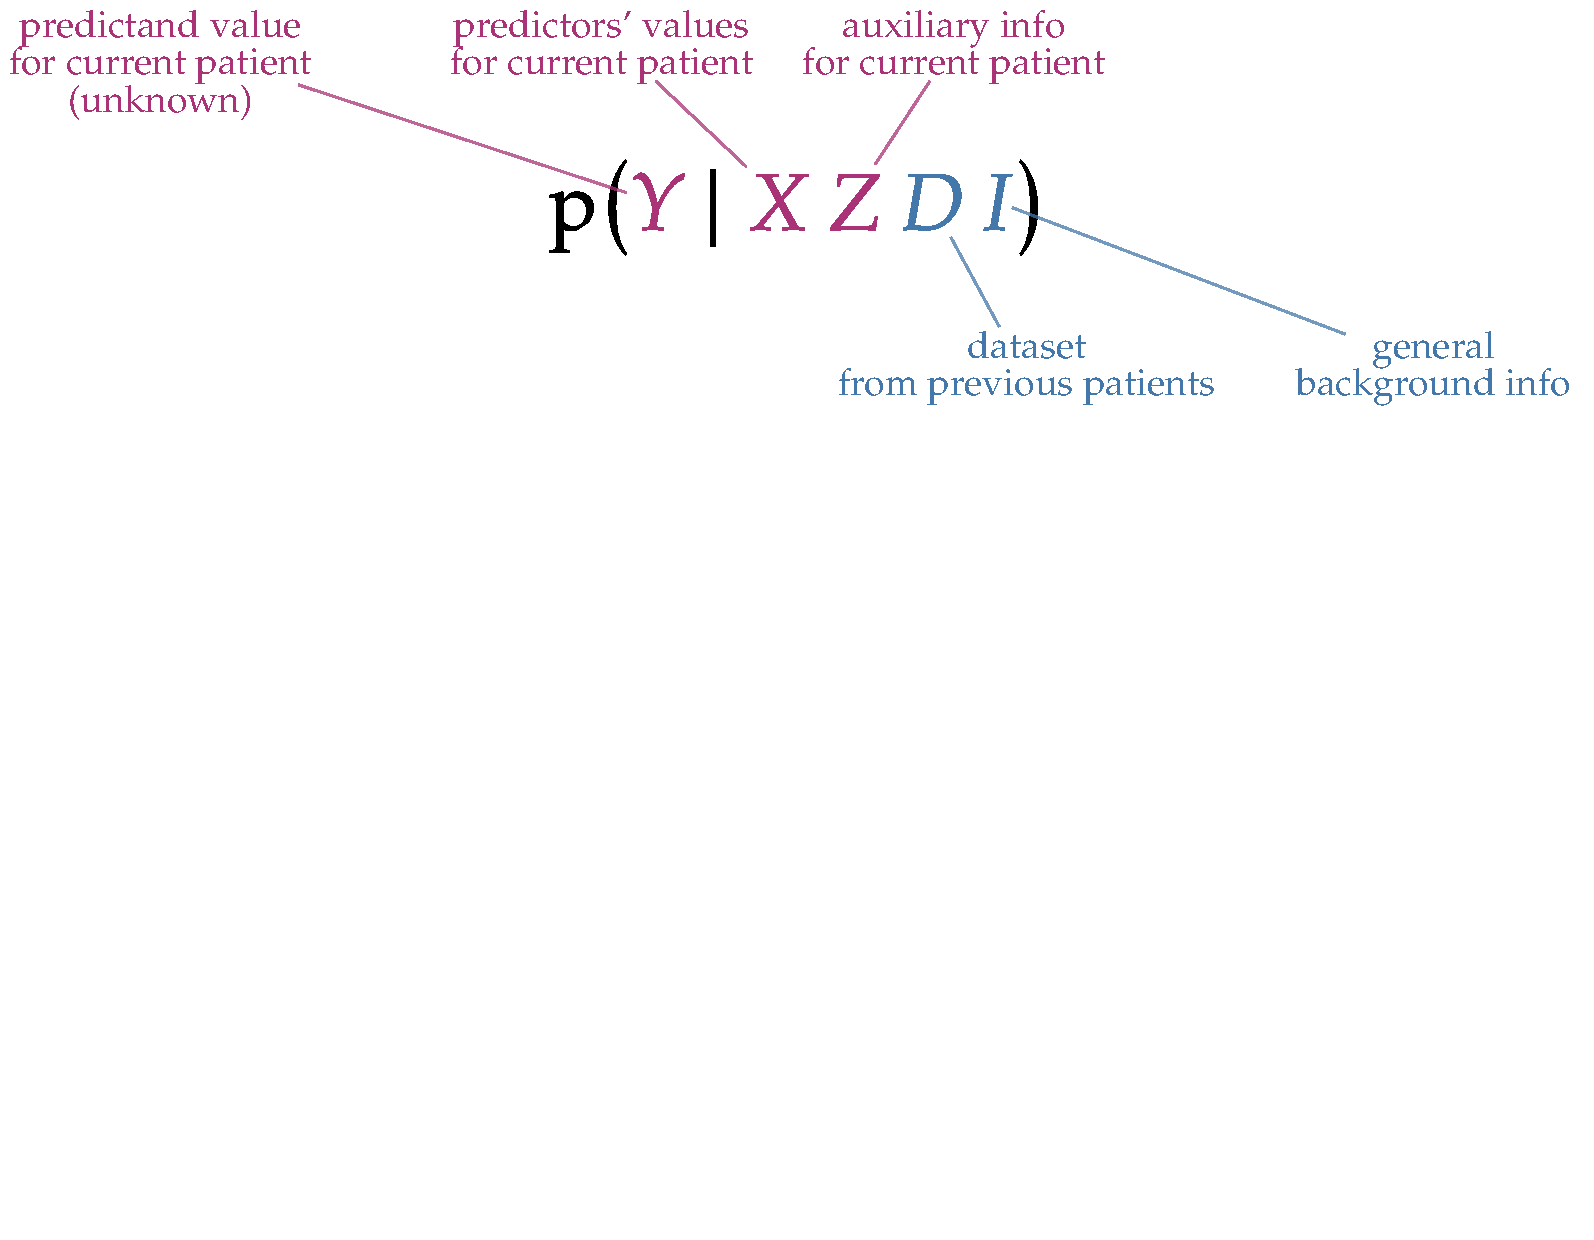
\includegraphics[width=0.67\linewidth]{p_scheme.pdf}%
\end{center}
It can be rewritten as follows, by the rules for conditional and marginal probabilities:
\begin{equation}
  \label{eq:prob_main}
  \p(Y \| X\,Z\,D\,I) \equiv
  \frac{\p(Y\, X \| Z\, D\, I)}{\sum_{Y}\p(Y\, X \| Z\, D\, I)}
\end{equation}

The \ljm\ calculates and outputs this probability in several different ways, as demanded by the clinician according to current patient's situation:
\begin{enumerate}[I.]
\item\label{item:prob_fully_exch} The patient and the datasets are mutually representative with regard to predictand \emph{and} all predictors; there is no auxiliary information:
  \begin{equation}
  \label{eq:prob_fully_exch}
  \p(Y \| X\,Z\,D\,I) \equiv
  \frac{\p(Y\, X \| Z\, D\, I)}{\sum_{Y}\p(Y\, X \| Z\, D\, I)} =
  \frac{\p(Y\, X \| D\, I)}{\sum_{Y}\p(Y\, X \| D\, I)}
\end{equation}

\item\label{item:prob_exch_givenX} The patient and the datasets are mutually representative with regards to predictand \emph{given} the predictors, but not with regard to the predictors alone; there is no auxiliary information:
  \begin{equation}
  \label{eq:prob_exch_givenX}
  \p(Y \| X\,Z\,D\,I) \equiv
  \frac{\p(Y\, X \| Z\, D\, I)}{\sum_{Y}\p(Y\, X \| Z\, D\, I)} =
  % \frac{\p(Y\| X \, D\, I)\ \p(X\| Z\, D\,I)}{\sum_{Y}\p(Y\| X \, Z\, D\, I)\
  % \p(X \| Z\, D\, I)} =
  \p(Y \| X\, D\, I)
\end{equation}

\item\label{item:prob_exch_givenY} The patient and the datasets are mutually representative with regards to predictors \emph{given} the predictand, but not with regard to the predictand alone; there is auxiliary information:
  \begin{equation}
  \label{eq:prob_exch_givenY}
  \p(Y \| X\,Z\,D\,I) \equiv
  \frac{\p(Y\, X \| Z\, D\, I)}{\sum_{Y}\p(Y\, X \| Z\, D\, I)} =
  \frac{\p(X\| Y \, D\, I)\ \p(Y\| Z\,I)}{\sum_{Y}\p(X\| Y \, D\, I)\
  \p(Y \| Z\, I)}
\end{equation}

\item\label{item:prob_exch_other} Other intermediate situations.
%   \begin{equation}
%   \label{eq:prob_exch_givenY}
%   \p(Y \| X\,Z\,D\,I) \equiv
%   \frac{\p(Y\, X \| Z\, D\, I)}{\sum_{Y}\p(Y\, X \| Z\, D\, I)} =
%   \frac{\p(X\| Y \, D\, I)\ \p(Y\| Z\,I)}{\sum_{Y}\p(X\| Y \, D\, I)\
%   \p(Y \| Z\, I)}
% \end{equation}

\end{enumerate}
The difference between situations~\ref{item:prob_fully_exch} and \ref{item:prob_exch_givenX} is that in the former the \ljm\ first updates what it learned from the dataset by including the patient's predictor values, which can rightly be considered as a new datapoint for that set; whereas such update is not done in the latter case. If the dataset has a large number of datapoints, the results from these two situations are typically numerically identical.
